%%%%%%%%%%%%  Generated using docx2latex.com  %%%%%%%%%%%%%%

%%%%%%%%%%%%  v2.0.0-beta  %%%%%%%%%%%%%%

\documentclass[12pt]{report}
\usepackage{amsmath}
\usepackage{latexsym}
\usepackage{amsfonts}
\usepackage[normalem]{ulem}
\usepackage{array}
\usepackage{amssymb}
\usepackage{graphicx}
\usepackage[backend=biber,
style=numeric,
sorting=none,
isbn=false,
doi=false,
url=false,
]{biblatex}\addbibresource{bibliography.bib}

\usepackage{subfig}
\usepackage{wrapfig}
\usepackage{wasysym}
\usepackage{enumitem}
\usepackage{adjustbox}
\usepackage{ragged2e}
\usepackage[svgnames,table]{xcolor}
\usepackage{tikz}
\usepackage{longtable}
\usepackage{changepage}
\usepackage{setspace}
\usepackage{hhline}
\usepackage{multicol}
\usepackage{tabto}
\usepackage{float}
\usepackage{multirow}
\usepackage{makecell}
\usepackage{fancyhdr}
\usepackage[toc,page]{appendix}
\usepackage[hidelinks]{hyperref}
\usetikzlibrary{shapes.symbols,shapes.geometric,shadows,arrows.meta}
\tikzset{>={Latex[width=1.5mm,length=2mm]}}
\usepackage{flowchart}\usepackage[paperheight=11.69in,paperwidth=8.26in,left=0.98in,right=0.98in,top=0.98in,bottom=0.98in,headheight=1in]{geometry}
\usepackage[utf8]{inputenc}
\usepackage[norsk]{babel}
\usepackage[T1]{fontenc}
\TabPositions{0.49in,0.98in,1.47in,1.96in,2.45in,2.94in,3.43in,3.92in,4.41in,4.9in,5.39in,5.88in,}

\urlstyle{same}


 %%%%%%%%%%%%  Set Depths for Sections  %%%%%%%%%%%%%%

% 1) Section 
% 1.1) SubSection
% 1.1.1) SubSubSection
% 1.1.1.1) Paragraph
% 1.1.1.1.1) Subparagraph


\setcounter{tocdepth}{5}
\setcounter{secnumdepth}{5}


 %%%%%%%%%%%%  Set Depths for Nested Lists created by \begin{enumerate}  %%%%%%%%%%%%%%


\setlistdepth{9}
\renewlist{enumerate}{enumerate}{9}
		\setlist[enumerate,1]{label=\arabic*)}
		\setlist[enumerate,2]{label=\alph*)}
		\setlist[enumerate,3]{label=(\roman*)}
		\setlist[enumerate,4]{label=(\arabic*)}
		\setlist[enumerate,5]{label=(\Alph*)}
		\setlist[enumerate,6]{label=(\Roman*)}
		\setlist[enumerate,7]{label=\arabic*}
		\setlist[enumerate,8]{label=\alph*}
		\setlist[enumerate,9]{label=\roman*}

\renewlist{itemize}{itemize}{9}
		\setlist[itemize]{label=$\cdot$}
		\setlist[itemize,1]{label=\textbullet}
		\setlist[itemize,2]{label=$\circ$}
		\setlist[itemize,3]{label=$\ast$}
		\setlist[itemize,4]{label=$\dagger$}
		\setlist[itemize,5]{label=$\triangleright$}
		\setlist[itemize,6]{label=$\bigstar$}
		\setlist[itemize,7]{label=$\blacklozenge$}
		\setlist[itemize,8]{label=$\prime$}



 %%%%%%%%%%%%  Header here  %%%%%%%%%%%%%%


\pagestyle{fancy}
\fancyhf{}
\cfoot{ 
\vspace{\baselineskip}
}
\renewcommand{\headrulewidth}{0pt}
\setlength{\topsep}{0pt}\setlength{\parindent}{0pt}
\renewcommand{\arraystretch}{1.3}


%%%%%%%%%%%%%%%%%%%% Document code starts here %%%%%%%%%%%%%%%%%%%%



\begin{document}


 %%%%%%%%%%%%  This Produces Table Of Contents %%%%%%%%%%%%%%

\tableofcontents
\addcontentsline{toc}{chapter}{Contents}


 %%%%%%%%%%%%  Starting New Page here %%%%%%%%%%%%%%

\newpage

\vspace{\baselineskip}\section*{Hva er Algoritmer (m.m)?}
\addcontentsline{toc}{section}{Hva er Algoritmer (m.m)?}
\textbf{En uformell definisjon}: En algoritme er en hvilket som helst \textbf{tydelig definert fremgangsmåte} som kan ta en verdi (eller en mengde verdier) som \textbf{input} og gir en verdi (eller en mengde verdier) som \textbf{output}. Det er en sekvens som transformerer input til output.\par


\vspace{\baselineskip}
\textbf{Beskrivelse av løsning}: Det finnes ingen verdensomspennende standard for å beskrive en algoritme. Du kan beskrive den med naturlig språk, som et dataprogram eller til og med ved hjelp av å tegne maskinvare (hardware) som løser problemet. Det eneste kravet er at du er presis når du beskriver.\par


\vspace{\baselineskip}
\textbf{Instanser}: Hver samling av input-verdier til et slikt problem kalles en \textbf{instans}. For eksempel kan man i en instans av problemet over ha input-verdier som er et veikart over Trondheim, og de to punktene kan være to geografiske punkter som tilsvarer NTNU Gløshaugen og NTNU Dragvoll.\par


\vspace{\baselineskip}
\textbf{Riktig eller uriktig?}: En algoritme kan være enten \textbf{riktig} eller \textbf{uriktig}. Dersom en algoritme er \textit{riktig}, vil den for alle tenkbare instanser (innenfor området vi har bestemt) gi riktig output; f.eks. er det bare å forvente at en sorteringsalgoritme ikke vil ha problem med å sortere alle mulige samlinger av positive heltall. Dersom den er \textit{uriktig}, vil den ikke gjøre det. F.eks. kan du ha funnet på en algoritme som løser alle sorteringsproblemer ved å vende rekken av tall du har fått baklengs. Dette vil for noen instanser gi riktig output, men bare for en brøkdel av alle mulige instanser.\par


\vspace{\baselineskip}
\textbf{Problem}: Et problem er en relasjon mellom input og output.\par

\textbf{Probleminstans}: En probleminstans er en bestemt input.\par

\textbf{In-place}: En algoritme er in-place når den operer på input dataen uten å måtte lage feks nye array for å løse problemet.\par

\textbf{Stabil}: At en algoritme er stabil vil si at hvis du sorterer en liste med tall, vil alltid tallet i forekomsten som var først i den opprinnelige listen komme først i den sorterte listen.\par

\textbf{Rekursjon}: Deler opp i mindre problemer, løser de og konstruerer til slutt en fullstendig løsning ut fra del-løsningene (bruker induksjonstrinn).\par

\begin{itemize}
	\item Merk: Bruker et induktivt premiss om at du kan løse de mindre problemene
\end{itemize}\par


\vspace{\baselineskip}
\textbf{Pseudopolynomialitet}: Gitt en algoritme som tar tallet n som input og har kjøretid O(n) – hvilken kompleksitetsklasse er dette? n betegner her ikke størrelsen på input, men er selv en del av inputen. Det vil si at størrelsen til n = antall bits som kreves = lg(n).\par

\begin{adjustwidth}{0.98in}{0.0in}
 \( n=2^{lg⁡ \left( n \right) }=2 \omega  \)  $ \Rightarrow $  NB: Eksponentiell kjøretid! \par

\end{adjustwidth}

Dukker ofte opp som lureoppgave på eksamen!\par


\vspace{\baselineskip}

\vspace{\baselineskip}

\vspace{\baselineskip}

\vspace{\baselineskip}

\vspace{\baselineskip}

\vspace{\baselineskip}

\vspace{\baselineskip}

\vspace{\baselineskip}
\textbf{Asymtpoisk notasjon}: Notasjon hvor man dropper konstanter og lavere ordens ledd\par


\vspace{\baselineskip}


%%%%%%%%%%%%%%%%%%%% Table No: 1 starts here %%%%%%%%%%%%%%%%%%%%


\begin{table}[H]
 			\centering
\begin{tabular}{p{0.59in}p{0.58in}p{4.52in}}
\hline
%row no:1
\multicolumn{1}{|p{0.59in}}{\textbf{Notasjon}} & 
\multicolumn{1}{|p{0.58in}}{\textbf{Kjøretid}} & 
\multicolumn{1}{|p{4.52in}|}{\textbf{Betydning}} \\
\hhline{---}
%row no:2
\multicolumn{1}{|p{0.59in}}{ \( o \left( n \right)  \) } & 
\multicolumn{1}{|p{0.58in}}{\Centering a < b} & 
\multicolumn{1}{|p{4.52in}|}{\cellcolor[HTML]{FFFFFF}{\fontsize{11pt}{13.2pt}\selectfont \textcolor[HTML]{222222}{S}trengere enn  \( O \) } \par \begin{itemize}
	\item {\fontsize{11pt}{13.2pt}\selectfont \textcolor[HTML]{222222}{o(g(n)) = $ \{ $ f(n): for enhver positiv konstant c>0, eksisterer det en konstant n\textsubscript{0} > 0 slik at 0 $ \leq $  f(n) < cg(n) for alle n $ \geq $  n\textsubscript{0}$ \} $ }} \par {\fontsize{11pt}{13.2pt}\selectfont \textcolor[HTML]{222222}{For eksempel: 2n = o(n\textsuperscript{2}), men 2n\textsuperscript{2} $ \neq $  o(n\textsuperscript{2})}}
\end{itemize}} \\
\hhline{---}
%row no:3
\multicolumn{1}{|p{0.59in}}{ \( O \left( n \right)  \) } & 
\multicolumn{1}{|p{0.58in}}{\Centering a $ \leq $  b} & 
\multicolumn{1}{|p{4.52in}|}{\cellcolor[HTML]{FFFFFF}gir en øvre grense for kjøretiden: \par \begin{itemize}
	\item {\fontsize{11pt}{13.2pt}\selectfont \textcolor[HTML]{222222}{O(g(n)) = $ \{ $ f(n): det eksisterer positive $\textbackslash$  konstanter c og n0 slik at 0 $ \leq $  f(n) $ \leq $  cg(n) for alle n $ \geq $  n\textsubscript{0}$ \} $ }}
\end{itemize}} \\
\hhline{---}
%row no:4
\multicolumn{1}{|p{0.59in}}{ \(  \Theta  \left( n \right)  \) } & 
\multicolumn{1}{|p{0.58in}}{\Centering a = b} & 
\multicolumn{1}{|p{4.52in}|}{\cellcolor[HTML]{FFFFFF}gir øvre og nedre grense for kjøretiden: \par \begin{itemize}
	\item {\fontsize{11pt}{13.2pt}\selectfont \textcolor[HTML]{222222}{$ \Theta $ (g(n)) = $ \{ $ f(n): det eksisterer positive konstanter c\textsubscript{1},c\textsubscript{2} og n\textsubscript{0} slik at 0$ \leq $  c\textsubscript{1}g(n) $ \leq $  f(n )$ \leq $  c\textsubscript{2}g(n) for alle n$ \geq $ n\textsubscript{0} $ \} $ }}
\end{itemize}} \\
\hhline{---}
%row no:5
\multicolumn{1}{|p{0.59in}}{ \(  \omega  \left( n \right)  \) } & 
\multicolumn{1}{|p{0.58in}}{\Centering {\fontsize{11pt}{13.2pt}\selectfont a > b}} & 
\multicolumn{1}{|p{4.52in}|}{\cellcolor[HTML]{FFFFFF}{\fontsize{11pt}{13.2pt}\selectfont \textcolor[HTML]{222222}{S}trengere enn  \(  \Omega  \) } \par \begin{itemize}
	\item {\fontsize{11pt}{13.2pt}\selectfont \textcolor[HTML]{222222}{$ \omega $ (g(n)) = $ \{ $ f(n): for enhver positiv konstant c > 0, eksisterer det en konstant n\textsubscript{0} > 0 slik at 0 $ \leq $  cg(n) < f(n) for alle n $ \geq $  n\textsubscript{0}$ \} $ }} \par For eksempel:  \( \frac{n^{2}}{2}  \) = $ \omega $ (n), men  \( \frac{n^{2}}{2} \)  $ \neq $  $ \omega $ (n\textsuperscript{2}).
\end{itemize}} \\
\hhline{---}
%row no:6
\multicolumn{1}{|p{0.59in}}{ \(  \Omega  \left( n \right)  \) } & 
\multicolumn{1}{|p{0.58in}}{\Centering a $ \geq $  b} & 
\multicolumn{1}{|p{4.52in}|}{\cellcolor[HTML]{FFFFFF}gir en nedre grense for kjøretiden: \par \begin{itemize}
	\item {\fontsize{11pt}{13.2pt}\selectfont \textcolor[HTML]{222222}{$ \Omega $ (g(n)) = $ \{ $ f(n): det eksisterer positive konstanter c og n\textsubscript{0} slik at 0$ \leq $  cg(n) $ \leq $  f(n) for alle n $ \geq $  n\textsubscript{0}$ \} $ }}
\end{itemize}} \\
\hhline{---}

\end{tabular}
 \end{table}


%%%%%%%%%%%%%%%%%%%% Table No: 1 ends here %%%%%%%%%%%%%%%%%%%%


\vspace{\baselineskip}
{\fontsize{13pt}{15.6pt}\selectfont \textbf{Illustrasjon:}\par}\par



%%%%%%%%%%%%%%%%%%%% Figure/Image No: 1 starts here %%%%%%%%%%%%%%%%%%%%


\begin{figure}[H]	\begin{subfigure}		\includegraphics[width=0.28\textwidth]{./media/image1.png}
	\end{subfigure}
~	\begin{subfigure}		\includegraphics[width=0.28\textwidth]{./media/image2.png}
	\end{subfigure}
~	\begin{subfigure}		\includegraphics[width=0.28\textwidth]{./media/image3.png}
	\end{subfigure}
~
\end{figure}


%%%%%%%%%%%%%%%%%%%% Figure/Image No: 1 Ends here %%%%%%%%%%%%%%%%%%%%

 \par


\vspace{\baselineskip}
{\fontsize{13pt}{15.6pt}\selectfont \textbf{Asymptotiske egenskaper:}\par}\par


\vspace{\baselineskip}
\begin{multicols}{2}


%%%%%%%%%%%%%%%%%%%% Figure/Image No: 2 starts here %%%%%%%%%%%%%%%%%%%%

\begin{figure}[H]
	\begin{Center}
		\includegraphics[width=3.13in,height=1.28in]{./media/image4.png}
	\end{Center}
\end{figure}


%%%%%%%%%%%%%%%%%%%% Figure/Image No: 2 Ends here %%%%%%%%%%%%%%%%%%%%

\par



%%%%%%%%%%%%%%%%%%%% Figure/Image No: 3 starts here %%%%%%%%%%%%%%%%%%%%

\begin{figure}[H]
	\begin{Center}
		\includegraphics[width=1.52in,height=1.05in]{./media/image5.png}
	\end{Center}
\end{figure}


%%%%%%%%%%%%%%%%%%%% Figure/Image No: 3 Ends here %%%%%%%%%%%%%%%%%%%%

\par


\vspace{\baselineskip}

\end{multicols}

\vspace{\baselineskip}

\vspace{\baselineskip}\section*{Kjøretid}
\addcontentsline{toc}{section}{Kjøretid}
\setlength{\parskip}{10.56pt}
Kjøretiden til en algoritme er et mål på hvor effektiv en algoritme er og uten tvil det viktigste.\par

\subsection*{Om kjøretider}
\addcontentsline{toc}{subsection}{Om kjøretider}
\textbf{Hvorfor trenger vi kjøretid?:} I en verden der datamaskiner var uendelig raske og du hadde uendelig med tilgjengelig lagringsplass, kunne du brukt en hvilken som helst \textit{riktig} algoritme for å løse et problem – uansett hvor lite gjennomtenkt den måtte være. Men, som du sikkert har merket, er vi ikke i denne verdenen. Derfor har vi kjøretider.\par

\textbf{Forklaring av kjøretid}: En kjøretid beskriver det asymptotiske forholdet mellom størrelsen på problemet og hvor lang tid det vil ta å løse det.\par


\vspace{\baselineskip}
\subsection*{Noen vanlige kjøretider}
\addcontentsline{toc}{subsection}{Noen vanlige kjøretider}


%%%%%%%%%%%%%%%%%%%% Table No: 2 starts here %%%%%%%%%%%%%%%%%%%%


\begin{table}[H]
 			\centering
\begin{tabular}{p{1.31in}p{1.42in}p{3.34in}}
\hline
%row no:1
\multicolumn{1}{p{1.31in}}{\textbf{Kompleksitet}} & 
\multicolumn{1}{p{1.42in}}{\textbf{Navn}} & 
\multicolumn{1}{p{3.34in}}{\textbf{Type}} \\
\hhline{---}
%row no:2
\multicolumn{1}{p{1.31in}}{$ \Theta $ (n!)} & 
\multicolumn{1}{p{1.42in}}{Factorial} & 
\multicolumn{1}{p{3.34in}}{Generell} \\
\hhline{---}
%row no:3
\multicolumn{1}{p{1.31in}}{ \(  \Omega  \left( k^{n} \) )} & 
\multicolumn{1}{p{1.42in}}{Eksponensiell} & 
\multicolumn{1}{p{3.34in}}{Generell} \\
\hhline{---}
%row no:4
\multicolumn{1}{p{1.31in}}{ \( O \left( n^{k} \) )} & 
\multicolumn{1}{p{1.42in}}{Polynomisk} & 
\multicolumn{1}{p{3.34in}}{Generell} \\
\hhline{---}
%row no:5
\multicolumn{1}{p{1.31in}}{$ \Theta $  \(  \left( n^{3} \) )} & 
\multicolumn{1}{p{1.42in}}{Kubisk} & 
\multicolumn{1}{p{3.34in}}{Tilfelle av polynomisk} \\
\hhline{---}
%row no:6
\multicolumn{1}{p{1.31in}}{$ \Theta $  \(  \left( n^{2} \) )} & 
\multicolumn{1}{p{1.42in}}{Kvadratisk} & 
\multicolumn{1}{p{3.34in}}{Tilfelle av polynomisk} \\
\hhline{---}
%row no:7
\multicolumn{1}{p{1.31in}}{ \(  \Theta  \left( nlgn \right)  \) } & 
\multicolumn{1}{p{1.42in}}{Loglineær} & 
\multicolumn{1}{p{3.34in}}{Kombinasjon av lineær og logaritmisk} \\
\hhline{---}
%row no:8
\multicolumn{1}{p{1.31in}}{$ \Theta $ (n)} & 
\multicolumn{1}{p{1.42in}}{Lineær} & 
\multicolumn{1}{p{3.34in}}{Generell} \\
\hhline{---}
%row no:9
\multicolumn{1}{p{1.31in}}{ \(  \Theta  \left( lgn \right)  \) } & 
\multicolumn{1}{p{1.42in}}{Logaritmisk} & 
\multicolumn{1}{p{3.34in}}{Generell} \\
\hhline{---}
%row no:10
\multicolumn{1}{p{1.31in}}{ \(  \Theta  \left(  \left( log_{b}n \right) ^{k} \right)  \) } & 
\multicolumn{1}{p{1.42in}}{Polylogaritmisk} & 
\multicolumn{1}{p{3.34in}}{?} \\
\hhline{---}
%row no:11
\multicolumn{1}{p{1.31in}}{$ \Theta $ (1)} & 
\multicolumn{1}{p{1.42in}}{Konstant} & 
\multicolumn{1}{p{3.34in}}{Generell} \\
\hhline{---}

\end{tabular}
 \end{table}


%%%%%%%%%%%%%%%%%%%% Table No: 2 ends here %%%%%%%%%%%%%%%%%%%%


\vspace{\baselineskip}

\vspace{\baselineskip}

\vspace{\baselineskip}\subsection*{Kjøretidsberegning}
\addcontentsline{toc}{subsection}{Kjøretidsberegning}
Rekursjon er en problemløsningsmetodikk som baserer seg på at løsningen på et problem er satt sammen av løsningene til mindre instanser av samme problem. Denne teknikken kommer til å gå igjen i mange av algoritmene i pensum.\par

Et av de aller vanligste eksemplene på rekursivitet er Fibonaccitallene, definert som:\par

\begin{Center}
F(n) = F(n$-$ 1) + F(n$-$ 2)
\end{Center}\par

\begin{Center}
F(0) = 0,  F(1) = 1
\end{Center}\par

\setlength{\parskip}{0.0pt}
Fibonaccitall n er altså definert som summen av de to foregående Fibonaccitallene.\par

\setlength{\parskip}{10.56pt}
Gode eksempler på rekursive algoritmer er Merge og Quick Sort og binærsøk. Vi finner også ofte rekursive løsninger ved bruk av dynamisk programmering.\par


\vspace{\baselineskip}
\subsection*{Splitt $\&$  hersk}
\addcontentsline{toc}{subsection}{Splitt $\&$  hersk}
Divide: Del problemet opp i subproblemer som er mindre instanser av det samme problemet.\par

Conquer: Løs subproblemene rekursivt, når subproblemene blir små nok (base case) kan vi løse de rett frem. \par

Combine: Kombiner løsningene av subproblemene til en løsning av problemet. Hvis det er et problem om ikke er en del av den rekursive løsningen antas den å være en del av combine-problemet.\par


\vspace{\baselineskip}
\subsection*{Variabelskifte}
\addcontentsline{toc}{subsection}{Variabelskifte}
Bytt ut m = lg n for å få enklere likninger. Får da n = 2m, og T(n) = T(2m) = S(m). Får da vanlige rekursjoner, uten lg n og andre vanskelige saker. Kan løse med iterasjonsmetoden, masterteoremet eller substitusjon, og så bytte tilbake til originale variabler. 

 %%%%%%%%%%%%  Starting New Page here %%%%%%%%%%%%%%

\newpage
\par

\subsection*{Masterteoremet}
\addcontentsline{toc}{subsection}{Masterteoremet}
Masterteoremet er en kokebokløsning for å finne kjøretiden til (mange) rekurrenser på formen\par

 \[ T \left( n \right) =aT \left( \frac{n}{b} \right) +f \left( n \right)  \] \par

\begin{Center}
a $ \geq $  1, b > 1
\end{Center}\par

\setlength{\parskip}{0.0pt}
Merk: en viktig egenskap vi kan utnytte når vi jobber med master teoremet er at  \( a^{logn}=n^{loga} \) .\par

Denne typen rekurrenser oppstår gjerne i sammenheng med splitt-og-hersk algoritmer, f.eks. Merge sort. Problemet deles opp i a deler av størrelse n/b, med f(n) arbeid for å gjøre selve oppdelinga, og å sette sammen resultatet av rekursive kall etter at disse er ferdige. I eksempelet med Merge sort, er f(n) arbeidet med å splitte lista i to underlister, og å flette sammen de to sorterte listene etter at de rekursive kallene er ferdige. Det å splitte skjer i konstant tid $ \Theta $ (1), mens det å flette sammen tar lineær tid $ \Theta $ (n). Vi kan altså sette f(n)=n. Siden vi til enhver tid deler listen opp i to deler, hver del n/2 er henholdsvis a=2 og b=2. For Merge sort har vi altså:\par

\begin{Center}
 \[ T \left( n \right) =2T \left( \frac{n}{2} \right) +n \] 
\end{Center}\par

\setlength{\parskip}{10.56pt}
Dersom vi ikke allerede visste kjøretiden til Merge sort, kunne vi funnet den ved å løse denne rekurrensen. Å løse rekurrensen kunne vi så brukt Masterteoremet til. \par

Fremgangsmåten for Masterteoremet er som følger:\par

\begin{enumerate}[label*=\arabic*.]
	\item Identifiser a,b,f(n)\par

	\item Regn ut log\textsubscript{b}a \par

	\item Konsulter tabellen under
\end{enumerate}\par

Tabell over de tre tilfellene av Masterteoremet: \par



%%%%%%%%%%%%%%%%%%%% Table No: 3 starts here %%%%%%%%%%%%%%%%%%%%


\begin{table}[H]
 			\centering
\begin{tabular}{p{0.96in}p{2.49in}p{2.61in}}
\hline
%row no:1
\multicolumn{1}{p{0.96in}}{Tilfelle} & 
\multicolumn{1}{p{2.49in}}{Krav} & 
\multicolumn{1}{p{2.61in}}{Løsning} \\
\hhline{---}
%row no:2
\multicolumn{1}{p{0.96in}}{1} & 
\multicolumn{1}{p{2.49in}}{f(n) $ \in $  O( \( n^{log_{b}a- \epsilon } \) )} & 
\multicolumn{1}{p{2.61in}}{T(n) $ \in $  $ \Theta $ ( \( n^{log_{b}a} \) )} \\
\hhline{---}
%row no:3
\multicolumn{1}{p{0.96in}}{2} & 
\multicolumn{1}{p{2.49in}}{f(n) $ \in $  $ \Theta $ ( \( n^{log_{b}a} \) log\textsuperscript{k}n)} & 
\multicolumn{1}{p{2.61in}}{T(n) $ \in $  $ \Theta $ ( \( n^{log_{b}a} \) log\textsuperscript{k+1}n) } \\
\hhline{---}
%row no:4
\multicolumn{1}{p{0.96in}}{3} & 
\multicolumn{1}{p{2.49in}}{f(n) $ \in $  $ \Omega $ ( \( n^{log_{b}a+ \epsilon } \right)  \) } & 
\multicolumn{1}{p{2.61in}}{T(n) $ \in $  $ \Theta $ (f(n))} \\
\hhline{---}

\end{tabular}
 \end{table}


%%%%%%%%%%%%%%%%%%%% Table No: 3 ends here %%%%%%%%%%%%%%%%%%%%


\vspace{\baselineskip}
\setlength{\parskip}{0.0pt}
Merk: $ \epsilon $  > 0\par


\vspace{\baselineskip}
Vi fortsetter eksempelet med Merge sort. Vi har funnet a=2, b=2, f(n)=n, da må log\textsubscript{b} a = log\textsubscript{2} 2 = 1. Vi har altså tilfelle 2,  f(n) $ \in $  $ \Theta $ (n\textsuperscript{1}) med løsning T(n)$ \in $ $ \Theta $ (n lgn)).\par


\vspace{\baselineskip}

\vspace{\baselineskip}


 %%%%%%%%%%%%  Starting New Page here %%%%%%%%%%%%%%

\newpage

\vspace{\baselineskip}\uline{Og på norsk betyr dette }\par

\begin{enumerate}
	\item Hvis f(n) < n\textsuperscript{log}\textsubscript{b}\textsuperscript{a }med en polynomisk faktor, så er T(n) = $ \Theta $ (n\textsuperscript{log}\textsubscript{b}\textsuperscript{a})\par

	\item Hvis f(n) = n\textsuperscript{log}\textsubscript{b}\textsuperscript{a } (samme polynomiske faktor), så er T(n) = $ \Theta $ (n\textsuperscript{log}\textsubscript{b}\textsuperscript{a} lg n) = $ \Theta $ (f(n) lg n)\par

	\item Hvis f(n) > n\textsuperscript{log}\textsubscript{b}\textsuperscript{a }med en polynomisk faktor OG af(n/b) $ \leq $  cf(n), så er T(n) = $ \Theta $ (f(n))
\end{enumerate}\par


\vspace{\baselineskip}
\setlength{\parskip}{6.0pt}
\subsubsection*{Eksempel}
\addcontentsline{toc}{subsubsection}{Eksempel}
\setlength{\parskip}{10.56pt}
Enda et eksempel, hentet fra kontinuasjonseksamen 2009:\par

Løs følgende rekurrens. Oppgi svaret i asymptotisk notasjon. Begrunn svaret kort.\par

\begin{Center}
 \[ T \left( n \right) =2T \left( \frac{n}{3} \right) +\frac{1}{n} \] 
\end{Center}\par


\vspace{\baselineskip}
\setlength{\parskip}{0.0pt}
Vi har a=2, b=3, f(n)=n\textsuperscript{-1}. Det gir log\textsubscript{b} a=log\textsubscript{3} 2 $ \approx $  0.63. Siden f(n)=n\textsuperscript{-1} er O(n\textsuperscript{63}), har vi tilfelle 1 og løsningen T(n) $ \in $  $ \Theta $ (n\textsuperscript{63}).

 %%%%%%%%%%%%  Starting New Page here %%%%%%%%%%%%%%

\newpage
\par

\section*{Grunnleggende datastrukturer}
\addcontentsline{toc}{section}{Grunnleggende datastrukturer}
\subsection*{Stacks and Queues (Dynamic Sets)}
\addcontentsline{toc}{subsection}{Stacks and Queues (Dynamic Sets)}
\setlength{\parskip}{10.56pt}
Stakker og køer er dynamiske sett med 2 viktige metoder, PUSH og POP, som betyr hhv. å legge til og fjerne et element. Merk at et POP-kall og et DELETE-kall er det samme.\par



%%%%%%%%%%%%%%%%%%%% Figure/Image No: 4 starts here %%%%%%%%%%%%%%%%%%%%

\begin{figure}[H]
	\begin{Center}
		\includegraphics[width=150pt,height=98.4pt]{./media/image6.png}
	\end{Center}
\end{figure}


%%%%%%%%%%%%%%%%%%%% Figure/Image No: 4 Ends here %%%%%%%%%%%%%%%%%%%%

\subsubsection*{Queue}
\addcontentsline{toc}{subsubsection}{Queue}
\setlength{\parskip}{0.0pt}
En queue er en FIFO (First In First Out) struktur. En\ kø implementeres som oftest som et array (gjerne et dynamisk array, likt Java sin ArrayList. En kø har egenskapene ENQUEUE og DEQUEUE.  Dette vil si at et Dequeue-kall til køen returnerer elementet som først ble satt inn.\par


\vspace{\baselineskip}
\setlength{\parskip}{10.56pt}

\vspace{\baselineskip}
\begin{multicols}{2}
\textbf{Enqueue}\par


\vspace{\baselineskip}


%%%%%%%%%%%%%%%%%%%% Figure/Image No: 5 starts here %%%%%%%%%%%%%%%%%%%%

\begin{figure}[H]
	\begin{Center}
		\includegraphics[width=2.4in,height=1.05in]{./media/image7.png}
	\end{Center}
\end{figure}


%%%%%%%%%%%%%%%%%%%% Figure/Image No: 5 Ends here %%%%%%%%%%%%%%%%%%%%

\par


\vspace{\baselineskip}
Insert-metode, kalles enqueue for en kø. \textit{Tail}-variabelen peker alltid på neste ledige plass i arrayet, så når vi enqueuer legger vi bare elementet rett inn. Vi må oppdatere \textit{tail-}variablen, hvis den er lik lengden av lista settes den til 1, hvis ikke inkrementeres den. Man må egentlig også sjekke for overflow, altså at køen er full. Da kan en sjekke om \textit{head }== \textit{tail }+ 1 (teknisk sett er det en ledig plass i køen da, men dette defineres for å kunne avgjøre når køen er tom).\par

\textbf{Dequeue}\par


\vspace{\baselineskip}


%%%%%%%%%%%%%%%%%%%% Figure/Image No: 6 starts here %%%%%%%%%%%%%%%%%%%%

\begin{figure}[H]
	\begin{Center}
		\includegraphics[width=2.57in,height=1.21in]{./media/image8.png}
	\end{Center}
\end{figure}


%%%%%%%%%%%%%%%%%%%% Figure/Image No: 6 Ends here %%%%%%%%%%%%%%%%%%%%

\par


\vspace{\baselineskip}
Vi sparer på det fremste elementet. Så setter vi \textit{head} til å være 1 dersom vi er på enden av lista, hvis ikke inkrementeres \textit{head}. Så returneres elementet som nettopp ble fjernet. Man må her egentlig sjekke for underflowerror, altså at lista er tom. Da kan en sjekke om \par

\textit{head} == \textit{tail.}\par


\vspace{\baselineskip}

\vspace{\baselineskip}

\end{multicols}

\vspace{\baselineskip}\subsubsection*{Stack}
\addcontentsline{toc}{subsubsection}{Stack}


%%%%%%%%%%%%%%%%%%%% Figure/Image No: 7 starts here %%%%%%%%%%%%%%%%%%%%

\begin{figure}[H]
	\begin{Center}
		\includegraphics[width=139.2pt,height=100.15pt]{./media/image9.png}
	\end{Center}
\end{figure}


%%%%%%%%%%%%%%%%%%%% Figure/Image No: 7 Ends here %%%%%%%%%%%%%%%%%%%%

\setlength{\parskip}{0.0pt}
En stakk er LIFO (Last In First Out) struktur. Stack implementeres oftest med et array, eller en lenket liste. En stack har egenskapene INSERT, PUSH og POP (DELETE).Et POP-kall til stakken returnerer elementet som sist ble satt inn.\par


\vspace{\baselineskip}

\vspace{\baselineskip}
\setlength{\parskip}{10.56pt}

\vspace{\baselineskip}
\begin{multicols}{2}
{\fontsize{13pt}{15.6pt}\selectfont \textbf{Stack-empty}\par}\par



%%%%%%%%%%%%%%%%%%%% Figure/Image No: 8 starts here %%%%%%%%%%%%%%%%%%%%

\begin{figure}[H]
	\begin{Center}
		\includegraphics[width=2.0in,height=1.1in]{./media/image10.png}
	\end{Center}
\end{figure}


%%%%%%%%%%%%%%%%%%%% Figure/Image No: 8 Ends here %%%%%%%%%%%%%%%%%%%%

{\fontsize{13pt}{15.6pt}\selectfont  \par}\par

Stakken har en variabel top som peker på hvor i arrayet det øverste elementet ligger. Når denne er null er stakken tom, og stack-empty returnerer true. \par

{\fontsize{13pt}{15.6pt}\selectfont \textbf{Push}\par}\par



%%%%%%%%%%%%%%%%%%%% Figure/Image No: 9 starts here %%%%%%%%%%%%%%%%%%%%

\begin{figure}[H]
	\begin{Center}
		\includegraphics[width=1.66in,height=0.61in]{./media/image11.png}
	\end{Center}
\end{figure}


%%%%%%%%%%%%%%%%%%%% Figure/Image No: 9 Ends here %%%%%%%%%%%%%%%%%%%%

{\fontsize{13pt}{15.6pt}\selectfont  \par}\par

Insert-operasjon, kalles push for stakker. Øker top-variablen med en, og legger til det nye elementet øverst i stakken. Dersom top blir større enn størrelsen på lista vil det utløse en error (overflow).\par

{\fontsize{13pt}{15.6pt}\selectfont \textbf{Pop}\par}\par



%%%%%%%%%%%%%%%%%%%% Figure/Image No: 10 starts here %%%%%%%%%%%%%%%%%%%%

\begin{figure}[H]
	\begin{Center}
		\includegraphics[width=2.57in,height=1.03in]{./media/image12.png}
	\end{Center}
\end{figure}


%%%%%%%%%%%%%%%%%%%% Figure/Image No: 10 Ends here %%%%%%%%%%%%%%%%%%%%

\par

Delete-operasjon, kalles pop for stakker. Hvis stakken er tom utløses en underflowerror. Hvis ikke minkes top med en og det elementet som nettopp ble fjernet blir returnert. Merk at den ikke tar inn noen elementer å fjerne, en stakk fjerner alltid det øverste elementet.\par


\vspace{\baselineskip}

\vspace{\baselineskip}

\vspace{\baselineskip}

\vspace{\baselineskip}

\vspace{\baselineskip}

\vspace{\baselineskip}

\vspace{\baselineskip}

\vspace{\baselineskip}

\end{multicols}

\vspace{\baselineskip}

\vspace{\baselineskip}

\vspace{\baselineskip}

\vspace{\baselineskip}

\vspace{\baselineskip}

\vspace{\baselineskip}

\vspace{\baselineskip}\subsection*{Lenkede lister}
\addcontentsline{toc}{subsection}{Lenkede lister}


%%%%%%%%%%%%%%%%%%%% Figure/Image No: 11 starts here %%%%%%%%%%%%%%%%%%%%

\begin{figure}[H]
	\begin{Center}
		\includegraphics[width=3.65in,height=0.44in]{./media/image13.png}
	\end{Center}
\end{figure}


%%%%%%%%%%%%%%%%%%%% Figure/Image No: 11 Ends here %%%%%%%%%%%%%%%%%%%%

Objektliknende, har en verdi og en peker til neste og forrige element i lista. Lagres ikke i et array, men som enkeltelementer som har en peker til neste og forrige element. Operasjonene blir ofte enkle, da det for det meste handler om å omdirigere pekerne.\par

I en dobbelt-lenket liste peker det også på det forrige elementet. Hvert objekt har helst to peker-variabler, next og prev. \par



%%%%%%%%%%%%%%%%%%%% Figure/Image No: 12 starts here %%%%%%%%%%%%%%%%%%%%

\begin{figure}[H]
	\begin{Center}
		\includegraphics[width=4.83in,height=0.57in]{./media/image14.png}
	\end{Center}
\end{figure}


%%%%%%%%%%%%%%%%%%%% Figure/Image No: 12 Ends here %%%%%%%%%%%%%%%%%%%%

\par


\vspace{\baselineskip}
\begin{multicols}{2}
\textbf{List-search}\par



%%%%%%%%%%%%%%%%%%%% Figure/Image No: 13 starts here %%%%%%%%%%%%%%%%%%%%

\begin{figure}[H]
	\begin{Center}
		\includegraphics[width=3.34in,height=1.16in]{./media/image15.png}
	\end{Center}
\end{figure}


%%%%%%%%%%%%%%%%%%%% Figure/Image No: 13 Ends here %%%%%%%%%%%%%%%%%%%%

\par

 \par

Søker lineært gjennom lista etter element med nøkkel k, hvis den ikke finnes, returneres NIL. Worst-case er at den må søke gjennom hele lista, altså $ \Theta $ (n). \par


\vspace{\baselineskip}
\textbf{List-insert}\par



%%%%%%%%%%%%%%%%%%%% Figure/Image No: 14 starts here %%%%%%%%%%%%%%%%%%%%

\begin{figure}[H]
	\begin{Center}
		\includegraphics[width=2.82in,height=1.43in]{./media/image16.png}
	\end{Center}
\end{figure}


%%%%%%%%%%%%%%%%%%%% Figure/Image No: 14 Ends here %%%%%%%%%%%%%%%%%%%%

\par

 \par

Insert-metode, setter elementet først i lista. Må da sette next-variabelen til det vi skal inserte til å peke på head, så må head sin prev peke på elementet vi skal legge til. Head må settes til å peke på elementet, og prev blir satt til NIL. Alt dette gjøres i O(1) tid. \par


\vspace{\baselineskip}
\textbf{List-delete}\par



%%%%%%%%%%%%%%%%%%%% Figure/Image No: 15 starts here %%%%%%%%%%%%%%%%%%%%

\begin{figure}[H]
	\begin{Center}
		\includegraphics[width=2.43in,height=1.3in]{./media/image17.png}
	\end{Center}
\end{figure}


%%%%%%%%%%%%%%%%%%%% Figure/Image No: 15 Ends here %%%%%%%%%%%%%%%%%%%%

\par

 \par

Omdirigere pekerne slik at elementet blir fjerna, og next og prev til elementet peker på hverandre og ikke x. Hvis vi ønsker å fjerne et element med en gitt nøkkel må vi først kalle på List-Search. \par


\vspace{\baselineskip}

\vspace{\baselineskip}

\vspace{\baselineskip}

\vspace{\baselineskip}

\vspace{\baselineskip}

\vspace{\baselineskip}

\vspace{\baselineskip}

\vspace{\baselineskip}

\vspace{\baselineskip}

\vspace{\baselineskip}

\vspace{\baselineskip}

\vspace{\baselineskip}

\vspace{\baselineskip}

\vspace{\baselineskip}

\vspace{\baselineskip}

\end{multicols}

\vspace{\baselineskip}

\vspace{\baselineskip}

\vspace{\baselineskip}
\subsubsection*{Kjøretider}
\addcontentsline{toc}{subsubsection}{Kjøretider}


%%%%%%%%%%%%%%%%%%%% Table No: 4 starts here %%%%%%%%%%%%%%%%%%%%


\begin{table}[H]
 			\centering
\begin{tabular}{p{3.4in}p{2.87in}}
\hline
%row no:1
\multicolumn{1}{p{3.4in}}{{\fontsize{13pt}{15.6pt}\selectfont Handling}} & 
\multicolumn{1}{p{2.87in}}{{\fontsize{13pt}{15.6pt}\selectfont Kjøretid}} \\
\hhline{--}
%row no:2
\multicolumn{1}{p{3.4in}}{Innsetting på starten} & 
\multicolumn{1}{p{2.87in}}{O(1)} \\
\hhline{--}
%row no:3
\multicolumn{1}{p{3.4in}}{Innsetting på slutten} & 
\multicolumn{1}{p{2.87in}}{O(n)} \\
\hhline{--}
%row no:4
\multicolumn{1}{p{3.4in}}{Oppslag} & 
\multicolumn{1}{p{2.87in}}{O(n)} \\
\hhline{--}
%row no:5
\multicolumn{1}{p{3.4in}}{Slette element} & 
\multicolumn{1}{p{2.87in}}{oppslagstid + O(1)} \\
\hhline{--}

\end{tabular}
 \end{table}


%%%%%%%%%%%%%%%%%%%% Table No: 4 ends here %%%%%%%%%%%%%%%%%%%%


\vspace{\baselineskip}

\vspace{\baselineskip}

\vspace{\baselineskip}

\vspace{\baselineskip}

\vspace{\baselineskip}
\setlength{\parskip}{15.0pt}

\vspace{\baselineskip}

\vspace{\baselineskip}

\vspace{\baselineskip}\subsection*{Hashtabeller}
\addcontentsline{toc}{subsection}{Hashtabeller}


%%%%%%%%%%%%%%%%%%%% Figure/Image No: 16 starts here %%%%%%%%%%%%%%%%%%%%

\begin{figure}[H]
\advance\leftskip 4.98in		\includegraphics[width=2.02in,height=1.75in]{./media/image18.png}
\end{figure}


%%%%%%%%%%%%%%%%%%%% Figure/Image No: 16 Ends here %%%%%%%%%%%%%%%%%%%%

\setlength{\parskip}{10.56pt}
Bruker modfisert nøkkel k som indeks h(k). Vi ønsker å tillate store nøkler uten å ha store tabeller. Vi kan da «knøvle» nøkkelen til å bli en akseptabel, tilsynelatende tilfeldig, indeks. Obs: Input til en hashfunksjon kan være en vilkårlig bitstreng, tolket som et tall. Vi kan godt hashe andre ting som strenger og mer kompliserte objekter. Vi stapper objektene inn i hashfunksjonen og får en gyldig indeks ut.  Det er mulig at samme nøkkel hasher til samme verdi, da har vi en kollisjon. Kan løses med kjeding (se under). Dersom x.key=m og h(m)=j der h er en hashfunksjon vil x være elementet, m nøkkelen og j hashen.\par

\subsubsection*{Kjeding (Chaining)}
\addcontentsline{toc}{subsubsection}{Kjeding (Chaining)}


%%%%%%%%%%%%%%%%%%%% Figure/Image No: 17 starts here %%%%%%%%%%%%%%%%%%%%

\begin{figure}[H]
\advance\leftskip 4.38in		\includegraphics[width=2.61in,height=2.11in]{./media/image19.png}
\end{figure}


%%%%%%%%%%%%%%%%%%%% Figure/Image No: 17 Ends here %%%%%%%%%%%%%%%%%%%%

Om to verdier hasher til samme indeks, så har vi en kollisjon; for å ta vare på begge verdiene, kan vi ha en lenket liste (f.eks.) i hver celle i tabellen.\par

\begin{itemize}
	\item Mange kollisjoner: Lineært lange lister \par

\begin{itemize}
	\item Søk vil ta lineær tid\par


\end{itemize}
	\item Anta lineært stor tabell\par

	\item Anta jevn, «tilfeldig» fordeling \par

\begin{itemize}
	\item Konstant forventet kjøretid!\par


\end{itemize}
	\item Statisk datasett?  Lag custom hashfunksjon!\par

\begin{itemize}
	\item Kan da garantere konstant kjøretid\par


\vspace{\baselineskip}
Definerer load factor $ \alpha $  = n/m, n=elementer, m=nøkler, altså gjennomsnittlig antall elementer per nøkkel. Worst-case hvis alle elementer hasher til samme nøkkel, $ \Theta $ (n).\par


\vspace{\baselineskip}
{\fontsize{13pt}{15.6pt}\selectfont \textbf{Pseudokode}: \par}\par



%%%%%%%%%%%%%%%%%%%% Figure/Image No: 18 starts here %%%%%%%%%%%%%%%%%%%%

\begin{figure}[H]
	\begin{Center}
		\includegraphics[width=3.37in,height=1.46in]{./media/image20.png}
	\end{Center}
\end{figure}


%%%%%%%%%%%%%%%%%%%% Figure/Image No: 18 Ends here %%%%%%%%%%%%%%%%%%%%

\par


\vspace{\baselineskip}

\vspace{\baselineskip}
\textbf{Amortisert analyse:} Gjennomsnittstiden en operasjon tar, fordi worst-case kan være for pessimistisk. Si worst-case har en viss kjøretid, men etter at worst-case har skjedd én gang er det veldig lenge til det kan skje igjen (f.eks. å fordoble et array for å ha plass til flere elementer). Amortisert analyse summerer kjøretidene for ulike input og situasjoner, og deler deretter på antall ganger den ble kjørt. Se på gjennomsnitt per operasjon etter at mange har blitt utført (gjennomsnitt av kjøretiden):\   \(  \sum _{i=0}^{h-1}2^{i}=2^{h}-1 \) \par


\vspace{\baselineskip}

\end{itemize}
\end{itemize}
\vspace{\baselineskip}\subsubsection*{Hashfunksjoner}
\addcontentsline{toc}{subsubsection}{Hashfunksjoner}

\vspace{\baselineskip}
\textbf{The division method}\par

\begin{Center}
h(k) = k mod m
\end{Center}\par

Vi tar altså resten etter å ha delt på m, som er størrelsen på tabellen. Er noen verdien for m man ikke burde velge, f.eks. 2p, mens et primtall ikke for nærme 2p er ofte et godt valg.\par


\vspace{\baselineskip}
\textbf{The multiplication method}\par

\begin{Center}
h(k) = $ \lfloor $ m (kA mod 1)$ \rfloor $ 
\end{Center}\par

A er et tall mellom 0 og 1, tar den fraksjonelle delen av kA og ganger med m, størrelsen på tabellen, runder ned til nærmeste heltall. (kA mod 1 = kA - $ \lfloor $ kA$ \rfloor $ ).\par


\vspace{\baselineskip}
\subsection*{Dynamiske tabeller}
\addcontentsline{toc}{subsection}{Dynamiske tabeller}
Tabeller som kan øke og minke i størrelse utifra hvor mange elementer det inneholder. Definerer load faktor ⍺ = antall elementer i tabellen delt på antall plasser. Sier noe om hvor mye plass i tabellen som blir brukt. Vil ikke at den skal være for lav, og når den nærmer seg en må vi utvide tabellen.\par


\vspace{\baselineskip}
Hva om en hashtabell blir for full? Eller hva med en stakk eller kø? Vi kan allokere nytt minne og kopiere, men det tar jo lineær tid ... så vi vil gjøre det sjelden!  Vi tar i, og allokerer mye minne\par


\vspace{\baselineskip}
\textbf{Table-insert}\par



%%%%%%%%%%%%%%%%%%%% Figure/Image No: 19 starts here %%%%%%%%%%%%%%%%%%%%

\begin{figure}[H]
	\begin{Center}
		\includegraphics[width=3.26in,height=2.23in]{./media/image21.png}
	\end{Center}
\end{figure}


%%%%%%%%%%%%%%%%%%%% Figure/Image No: 19 Ends here %%%%%%%%%%%%%%%%%%%%

\par

T.size = antall plasser i tabellen\par

T.num = antall plasser brukt i tabellen\par

T.table = tabellen\par


\vspace{\baselineskip}
Hvis size er null oppretter vi tabellen og setter size til 1. Hvis num==size er tabellen full og vi lager en ny tabell med dobbelt så mange plasser og kopierer over elementene. Frigjør den gamle tabellen og lagrer den nye i T.table. Uavhengig av dette, til slutt settes elementet inn i tabellen og num økes med 1. 

 %%%%%%%%%%%%  Starting New Page here %%%%%%%%%%%%%%

\newpage
\par

\section*{Sortering}
\addcontentsline{toc}{section}{Sortering}
Stort sett kategoriserer vi sorteringsalgoritmer inn i to grupper; sammenligningsbaserte og distribuerte/ikke-sammenligningsbaserte.\par


\vspace{\baselineskip}
\subsection*{Stabilitet}
\addcontentsline{toc}{subsection}{Stabilitet}
En sorteringsalgoritme kan sies å være stabil dersom rekkefølgen av like elementer i listen som skal sorteres blir bevart i løpet av algoritmen. Altså at for de elementene som er like, vil det elementet som var først i input-arrayet være først i output-arrayet.  Eksempel, dersom vi har listen:\par

\begin{Center}
[B1,C1,C2,A1]
\end{Center}\par

og sorterer den med en eller annen algoritme, og de to like elementene står i samme rekkefølge etter sorteringen, har vi en stabil sorteringsalgoritme.\par

\begin{Center}
[A1,B1,C1,C2]
\end{Center}\par

\setlength{\parskip}{0.0pt}
Altså har vi at selv om verdien til C1 og C2 er den samme så blir C1 sortert før C2.\par


\vspace{\baselineskip}
\subsection*{Sammenligningsbaserte sorteringsalgoritmer}
\addcontentsline{toc}{subsection}{Sammenligningsbaserte sorteringsalgoritmer}
Alle sorteringsalgoritmer som baserer seg på å sammenligne to elementer for å avgjøre hvilket av de to som skal komme først i en sekvens, kaller vi sammenligningsbasert. Sammenlikningsbasert sortering: baserer sorteringen kun på sammenlikninger mellom elementene. Alle sammenlikningsbaserte sorteringsalgoritmer har en nedre grense på $ \Omega $ (n lg n). Heapsort og merge sort er optimale sammenlikningsbaserte sorteringsalgoritmer siden de har en øvre grense O(n lg n). Eks. på sammenlikningsbaserte sorteringsalgoritmer er insertion sort, merge sort, quicksort. \par


\vspace{\baselineskip}
For n elementer i en liste, finnes det n! permutasjoner. For hvert ja/nei-spørsmål vi stiller, dobler hva vi kan skille mellom (halveres hva vi står igjen med). \par

\begin{Center}
2\textsuperscript{T(n)} $ \geq $  n!
\end{Center}\par

\begin{Center}
T(n) $ \geq $  lg n!
\end{Center}\par

lg n! er antall halveringer fra n! til 1. For maks uflaks kan vi ikke gjøre det bedre med sammenlikningsbaserte sorteringsalgoritmer, fordi vi må sammenlikne lg n! ganger. Blir altså en nedre grense. \par

\begin{Center}
T\textsubscript{w}(n) = $ \Omega $ (lg n!) = $ \Omega $ (n lg n) $\ast$ 
\end{Center}\par

$\ast$ Stirlings approksimasjon: n! $ \geq $  (n/e)\textsuperscript{n} => lg n! $ \geq $  n lg n - n lg e = $ \Omega $ (n lg n).\par


\vspace{\baselineskip}

\vspace{\baselineskip}

\vspace{\baselineskip}

\vspace{\baselineskip}
\setlength{\parskip}{6.0pt}

\vspace{\baselineskip}\subsubsection*{Merge sort}
\addcontentsline{toc}{subsubsection}{Merge sort}
\setlength{\parskip}{10.56pt}
Merge sort er en splitt-og-hersk algoritme. Merge Sort er effektiv. Deler opp problemet i stadig mindre biter, og når bitene er små nok flettes de sammen i sortert rekkefølge. Mergesort gjør altså sorteringsarbeidet før det rekursive kallet. Merk: kan ikke bruke DP på merge sort siden det ikke er noen overlappende delproblemer.\par

Metode: «Divide $\&$  conquer», merging, sammenligningsbasert\par



%%%%%%%%%%%%%%%%%%%% Table No: 5 starts here %%%%%%%%%%%%%%%%%%%%


\begin{table}[H]
 			\centering
\begin{tabular}{p{1.2in}p{1.68in}p{1.42in}p{0.73in}p{0.63in}}
\hline
%row no:1
\multicolumn{1}{p{1.2in}}{{\fontsize{13pt}{15.6pt}\selectfont Best Case}} & 
\multicolumn{1}{p{1.68in}}{{\fontsize{13pt}{15.6pt}\selectfont Average Case}} & 
\multicolumn{1}{p{1.42in}}{{\fontsize{13pt}{15.6pt}\selectfont Worst Case}} & 
\multicolumn{1}{p{0.73in}}{{\fontsize{13pt}{15.6pt}\selectfont Stabil}} & 
\multicolumn{1}{p{0.63in}}{{\fontsize{13pt}{15.6pt}\selectfont Space}} \\
\hhline{-----}
%row no:2
\multicolumn{1}{p{1.2in}}{ \( O \left( n lgn \right)  \) } & 
\multicolumn{1}{p{1.68in}}{ \( O \left( n lgn \right)  \) } & 
\multicolumn{1}{p{1.42in}}{ \( O \left( n lgn \right)  \) } & 
\multicolumn{1}{p{0.73in}}{{\fontsize{13pt}{15.6pt}\selectfont Ja}} & 
\multicolumn{1}{p{0.63in}}{{\fontsize{14pt}{16.8pt}\selectfont O(n)}} \\
\hhline{-----}

\end{tabular}
 \end{table}


%%%%%%%%%%%%%%%%%%%% Table No: 5 ends here %%%%%%%%%%%%%%%%%%%%



%%%%%%%%%%%%%%%%%%%% Figure/Image No: 20 starts here %%%%%%%%%%%%%%%%%%%%

\begin{figure}[H]
\advance\leftskip 4.04in		\includegraphics[width=3.23in,height=2.27in]{./media/image22.png}
\end{figure}


%%%%%%%%%%%%%%%%%%%% Figure/Image No: 20 Ends here %%%%%%%%%%%%%%%%%%%%

\par

\begin{enumerate}[label*=\arabic*.]
	\item Sorter venstre halvdel rekursivt\par

\begin{enumerate}
	\item Todel listen rekursivt til hver liste inneholder 1 element$\ast$ 
\end{enumerate}\par

	\item Sorter høyre halvdel rekursivt\par

\begin{enumerate}
	\item Todel listen rekursivt til hver liste inneholder 1 element$\ast$  
\end{enumerate}\par

	\item Flett sammen underlistene.
\end{enumerate}\par


\vspace{\baselineskip}
$\ast$ (En liste med ett element er per definisjon sortert) \par

I praksis blir dette gjerne implementert rekursivt. Merge funksjonen kjører i lineær tid. For å analysere kjøretiden til Merge sort kan vi sette opp følgende rekurrens:\par

\begin{Center}
T(n) = 2T(n/2)+n
\end{Center}\par

\setlength{\parskip}{0.0pt}
Altså 2 ganger tiden det tar å sortere en liste av lengde n/2 pluss tiden det tar å flette de to listene. Se \href{https://www.wikipendium.no/TDT4120_Algoritmer_og_datastrukturer/nb/}{\textcolor[HTML]{006699}{Masterteoremet}} for hvordan vi kan løse denne rekurrensen og finne kjøretiden O(nlogn).\par

De fleste implementasjoner av Merge sort er stabile. På grunn av at algoritmen hele tiden lager nye underlister, trenger den O(n) ekstra plass i minnet.\par


\vspace{\baselineskip}
{\fontsize{13pt}{15.6pt}\selectfont \textbf{Pseudokode:}\par}\par


\vspace{\baselineskip}
\begin{multicols}{2}


%%%%%%%%%%%%%%%%%%%% Figure/Image No: 21 starts here %%%%%%%%%%%%%%%%%%%%

\begin{figure}[H]
	\begin{Center}
		\includegraphics[width=2.07in,height=1.08in]{./media/image23.png}
	\end{Center}
\end{figure}


%%%%%%%%%%%%%%%%%%%% Figure/Image No: 21 Ends here %%%%%%%%%%%%%%%%%%%%

\par


\vspace{\baselineskip}

\vspace{\baselineskip}


%%%%%%%%%%%%%%%%%%%% Figure/Image No: 22 starts here %%%%%%%%%%%%%%%%%%%%

\begin{figure}[H]
	\begin{Center}
		\includegraphics[width=2.88in,height=2.42in]{./media/image24.png}
	\end{Center}
\end{figure}


%%%%%%%%%%%%%%%%%%%% Figure/Image No: 22 Ends here %%%%%%%%%%%%%%%%%%%%


\end{multicols}
\par

\setlength{\parskip}{6.0pt}

\vspace{\baselineskip}\subsubsection*{Quicksort}
\addcontentsline{toc}{subsubsection}{Quicksort}
\setlength{\parskip}{10.56pt}
Quick Sort er enda en $``$split-og-hersk$"$ -algoritme. Man starter gjerne Quick Sort ved å randomisere lista. Den starter med å velge et pivotelement. Den deler deretter lista i to partisjoner: en med elementene som er mindre eller lik pivo- ten, og en med elementene som er større en pivot. Deretter kaller den seg selv rekursivt på de to partisjonene. Deretter fletter man sammen de to partisjonene. Quicksort gjør altså sorteringsarbeidet før det rekursive kallet. Krav om at elementene i lista må kunne sammenliknes\par

Metode: «Divide $\&$  conquer», partisjonering, sammenligning, in-place\par



%%%%%%%%%%%%%%%%%%%% Table No: 6 starts here %%%%%%%%%%%%%%%%%%%%


\begin{table}[H]
 			\centering
\begin{tabular}{p{1.13in}p{1.59in}p{1.34in}p{0.69in}p{0.91in}}
\hline
%row no:1
\multicolumn{1}{p{1.13in}}{{\fontsize{13pt}{15.6pt}\selectfont Best Case}} & 
\multicolumn{1}{p{1.59in}}{{\fontsize{13pt}{15.6pt}\selectfont Average Case}} & 
\multicolumn{1}{p{1.34in}}{{\fontsize{13pt}{15.6pt}\selectfont Worst Case}} & 
\multicolumn{1}{p{0.69in}}{{\fontsize{13pt}{15.6pt}\selectfont Stabil}} & 
\multicolumn{1}{p{0.91in}}{{\fontsize{13pt}{15.6pt}\selectfont Space}} \\
\hhline{-----}
%row no:2
\multicolumn{1}{p{1.13in}}{ \( O \left( n lgn \right)  \) } & 
\multicolumn{1}{p{1.59in}}{ \( O \left( n lgn \right)  \) } & 
\multicolumn{1}{p{1.34in}}{ \( O \left( n^{2} \right)  \) } & 
\multicolumn{1}{p{0.69in}}{{\fontsize{13pt}{15.6pt}\selectfont Nei}} & 
\multicolumn{1}{p{0.91in}}{ \( O \left( n lgn \right)  \) } \\
\hhline{-----}

\end{tabular}
 \end{table}


%%%%%%%%%%%%%%%%%%%% Table No: 6 ends here %%%%%%%%%%%%%%%%%%%%

\setlength{\parskip}{0.0pt}
Konseptet med et pivot-element står sentralt i quicksort. For hver iterasjon velger en seg et pivot-element og sorterer resten av elementene basert på om de er større eller lavere enn pivot-elementet. (Hvis pivot-elementet velges tilfeldig kalles algoritmen Randomized-Quicksort.)\par

\textbf{\uline{Fremgangsmåte}}:\par

\begin{enumerate}[label*=\arabic*.]
	\item \textbf{Divide}: Del opp arrayer i to subarrays, slik at hvert element i det første er mindre eller lik en pivot x, og hvert element i det andre er større enn x.\par

	\item \textbf{Conquer}: Sorter subarrayene utifra om de er større eller mindre enn piv, ved å rekursivt kalle quicksort\par

	\item \textbf{Combine}: Arrayene er sortert, og alle elementene i det ene er mindre enn alle elementene i det andre. Hele arrayet A er dermed sortert.
\end{enumerate}\par

Kjøretidsanalysen av Quicksort blir noe vanskeligere enn for Merge sort, ettersom størrelsen på listene som sorteres rekursivt vil avhenge av hvilken pivot vi velger. Det å velge en god pivot er en kunst i seg selv. Den naive fremgangsmåten med å slavisk velge det første elementet, kan lett utnyttes av en adversary, ved å gi en liste som er omvendt sortert som input. I dette tilfellet vil kjøretiden bli $ \Theta $ (n\textsuperscript{2}). Vi kan motvirke dette ved å velge en tilfeldig pivot i stedet.\par

\paragraph*{Pseudokode:}
\addcontentsline{toc}{paragraph}{Pseudokode:}

\vspace{\baselineskip}
\begin{multicols}{2}


%%%%%%%%%%%%%%%%%%%% Figure/Image No: 23 starts here %%%%%%%%%%%%%%%%%%%%

\begin{figure}[H]
	\begin{Center}
		\includegraphics[width=2.55in,height=1.2in]{./media/image25.png}
	\end{Center}
\end{figure}


%%%%%%%%%%%%%%%%%%%% Figure/Image No: 23 Ends here %%%%%%%%%%%%%%%%%%%%

\par



%%%%%%%%%%%%%%%%%%%% Figure/Image No: 24 starts here %%%%%%%%%%%%%%%%%%%%

\begin{figure}[H]
	\begin{Center}
		\includegraphics[width=2.67in,height=1.94in]{./media/image26.png}
	\end{Center}
\end{figure}


%%%%%%%%%%%%%%%%%%%% Figure/Image No: 24 Ends here %%%%%%%%%%%%%%%%%%%%


\end{multicols}
\par


\vspace{\baselineskip}

\vspace{\baselineskip}

\vspace{\baselineskip}

\vspace{\baselineskip}

\vspace{\baselineskip}
{\fontsize{14pt}{16.8pt}\selectfont \textbf{Partition}\par}\par


\vspace{\baselineskip}


%%%%%%%%%%%%%%%%%%%% Figure/Image No: 25 starts here %%%%%%%%%%%%%%%%%%%%


\begin{figure}[H]	\begin{subfigure}		\includegraphics[width=0.45\textwidth]{./media/image27.png}
	\end{subfigure}
~	\begin{subfigure}		\includegraphics[width=0.45\textwidth]{./media/image27.png}
	\end{subfigure}
~
\end{figure}


%%%%%%%%%%%%%%%%%%%% Figure/Image No: 25 Ends here %%%%%%%%%%%%%%%%%%%%

\par


\vspace{\baselineskip}
{\fontsize{14pt}{16.8pt}\selectfont \textbf{Worst-case}\par}\par

Får et subproblem med n-1 elementer i det ene arrayet og 0 i det andre. Hvis dette skjer for hvert rekursivt kall, og en partition tar $ \Theta $ (n) tid, vil kjøretiden være gitt ved\par

T(n) = T(n-1) + $ \Theta $ (n)\par

\ \ \ \ \ \ \  = T(n-2) + $ \Theta $ (n) + $ \Theta $ (n) = T(n-2) + 2$ \Theta $ (n)\par

\ \ \ \ \ \ \  = T(n-3) + 3$ \Theta $ (n)\par

\ \ \ \ \ \ \  = $ \ldots $  = T(n-(n-1)) + (n-1)$ \Theta $ (n) = $ \Theta $ (n\textsuperscript{2})\par

Dette er det samme som insertion sort, og skjer når arrayet allerede er sortert (eller omvendt sortert). \par


\vspace{\baselineskip}
{\fontsize{14pt}{16.8pt}\selectfont \textbf{Best-case}\par}\par

Hvis den deler arrayet midt på hver gang, blir størrelsen på subarrayene n/2 og n/2-1, og vi får kjøretid\par

T(n) = 2T(n/2) + $ \Theta $ (n) = $ \Theta $ (n lg n)\par


\vspace{\baselineskip}

\vspace{\baselineskip}

\vspace{\baselineskip}

\vspace{\baselineskip}

\vspace{\baselineskip}

\vspace{\baselineskip}

\vspace{\baselineskip}

\vspace{\baselineskip}

\vspace{\baselineskip}

\vspace{\baselineskip}

\vspace{\baselineskip}


 %%%%%%%%%%%%  Starting New Page here %%%%%%%%%%%%%%

\newpage

\vspace{\baselineskip}\setlength{\parskip}{6.0pt}
\subsubsection*{Quicksort (Randomized)}
\addcontentsline{toc}{subsubsection}{Quicksort (Randomized)}

\vspace{\baselineskip}
En randomisert versjon av quicksort. Velg pivot (dele-element) tilfeldig fra arrayet istedenfor å alltid ta det bakerste. Den krever at elementene i lista må kunne sammenliknes. Antar at elementene er distinkte. Algoritmen randomiseres, slik at samme dårlige input ikke alltid gir dårlig kjøretid. \par


\vspace{\baselineskip}

\vspace{\baselineskip}
\textbf{Pseudokode:}\par


\vspace{\baselineskip}
\begin{multicols}{2}


%%%%%%%%%%%%%%%%%%%% Figure/Image No: 26 starts here %%%%%%%%%%%%%%%%%%%%

\begin{figure}[H]
	\begin{Center}
		\includegraphics[width=3.57in,height=1.04in]{./media/image28.png}
	\end{Center}
\end{figure}


%%%%%%%%%%%%%%%%%%%% Figure/Image No: 26 Ends here %%%%%%%%%%%%%%%%%%%%

\par



%%%%%%%%%%%%%%%%%%%% Figure/Image No: 27 starts here %%%%%%%%%%%%%%%%%%%%

\begin{figure}[H]
	\begin{Center}
		\includegraphics[width=3.1in,height=1.01in]{./media/image29.png}
	\end{Center}
\end{figure}


%%%%%%%%%%%%%%%%%%%% Figure/Image No: 27 Ends here %%%%%%%%%%%%%%%%%%%%

\par


\vspace{\baselineskip}

\end{multicols}

\vspace{\baselineskip}
Randomized-partition velger tilfeldig pivot, bytter så bakerste element med dette. Kall på originale partition.\par

 \par

{\fontsize{14pt}{16.8pt}\selectfont \textbf{Worst-case og best-case}\par}\par

Samme som Quicksort\par



 %%%%%%%%%%%%  Starting New Page here %%%%%%%%%%%%%%

\newpage

\vspace{\baselineskip}\subsubsection*{Heapsort}
\addcontentsline{toc}{subsubsection}{Heapsort}
\setlength{\parskip}{0.0pt}
Heapsort benytter seg av en heap som datastruktur. Bygger en max-heap av alle ele- mentene sik at hver node sine barn er mindre enn den selv. Det øverste elementet er alltid det største. Deretter plukkes det øverste elemtentet ut, for så å sortere heapen igjen, og ta ut det øverste elementet igjen. Fortsetter til heapen er tom.\par

\textbf{Input}: Sekvens med tall, a1, a2, $ \ldots $ , an.\par

\textbf{Output}: Permutasjon av tallene slik at a’1 $ \leq $  a’2 $ \leq $  $ \ldots $  $ \leq $  a’n\par


\vspace{\baselineskip}
Metode: Seleksjon, sammenligningsbasert, prioritetskø, in-place\par



%%%%%%%%%%%%%%%%%%%% Table No: 7 starts here %%%%%%%%%%%%%%%%%%%%


\begin{table}[H]
 			\centering
\begin{tabular}{p{1.37in}p{1.36in}p{1.34in}p{0.73in}p{0.87in}}
\hline
%row no:1
\multicolumn{1}{p{1.37in}}{{\fontsize{13pt}{15.6pt}\selectfont BC}} & 
\multicolumn{1}{p{1.36in}}{{\fontsize{13pt}{15.6pt}\selectfont AC}} & 
\multicolumn{1}{p{1.34in}}{{\fontsize{13pt}{15.6pt}\selectfont WC}} & 
\multicolumn{1}{p{0.73in}}{{\fontsize{13pt}{15.6pt}\selectfont SC}} & 
\multicolumn{1}{p{0.87in}}{{\fontsize{13pt}{15.6pt}\selectfont Stable}} \\
\hhline{-----}
%row no:2
\multicolumn{1}{p{1.37in}}{{\fontsize{14pt}{16.8pt}\selectfont $ \Omega $  \(  \left( n lgn \right)  \) }} & 
\multicolumn{1}{p{1.36in}}{{\fontsize{14pt}{16.8pt}\selectfont $ \Theta $  \(  \left( n lgn \right)  \) }} & 
\multicolumn{1}{p{1.34in}}{ \( O \left( n lgn \right)  \) } & 
\multicolumn{1}{p{0.73in}}{{\fontsize{14pt}{16.8pt}\selectfont O(1)}} & 
\multicolumn{1}{p{0.87in}}{{\fontsize{13pt}{15.6pt}\selectfont Nei}} \\
\hhline{-----}

\end{tabular}
 \end{table}


%%%%%%%%%%%%%%%%%%%% Table No: 7 ends here %%%%%%%%%%%%%%%%%%%%


\vspace{\baselineskip}
{\fontsize{13pt}{15.6pt}\selectfont \textbf{Pseudokode\par}:}\par


\vspace{\baselineskip}
\begin{multicols}{2}


%%%%%%%%%%%%%%%%%%%% Figure/Image No: 28 starts here %%%%%%%%%%%%%%%%%%%%

\begin{figure}[H]
	\begin{Center}
		\includegraphics[width=2.42in,height=1.35in]{./media/image30.png}
	\end{Center}
\end{figure}


%%%%%%%%%%%%%%%%%%%% Figure/Image No: 28 Ends here %%%%%%%%%%%%%%%%%%%%

\par


\vspace{\baselineskip}


%%%%%%%%%%%%%%%%%%%% Figure/Image No: 29 starts here %%%%%%%%%%%%%%%%%%%%

\begin{figure}[H]
	\begin{Center}
		\includegraphics[width=2.42in,height=0.88in]{./media/image31.png}
	\end{Center}
\end{figure}


%%%%%%%%%%%%%%%%%%%% Figure/Image No: 29 Ends here %%%%%%%%%%%%%%%%%%%%

\par



%%%%%%%%%%%%%%%%%%%% Figure/Image No: 30 starts here %%%%%%%%%%%%%%%%%%%%

\begin{figure}[H]
	\begin{Center}
		\includegraphics[width=2.35in,height=2.15in]{./media/image32.png}
	\end{Center}
\end{figure}


%%%%%%%%%%%%%%%%%%%% Figure/Image No: 30 Ends here %%%%%%%%%%%%%%%%%%%%

\par


\vspace{\baselineskip}

\end{multicols}

\vspace{\baselineskip}
\textbf{Fremgangsmåte:}\par

Først bygger vi en max-heap. Siden rota til heapen er det største elementet, legger vi dette bakerst i lista, dekrementerer heap-size-variabelen, som begrenser heapen til A[1..heap-size]. Nå er altså det som var rota, plassert bakerst, og ikke lengre med i heapen (selv om det er med i lista). Elementet som var bakerst, blir plassert i rota, så vi må kalle på max-heapify for denne nye rota. \par


\vspace{\baselineskip}
Se heaps for forklaring på Max-heapify og Build-max-heap.

 %%%%%%%%%%%%  Starting New Page here %%%%%%%%%%%%%%

\newpage
\par

\setlength{\parskip}{6.0pt}
\subsubsection*{Insertion Sort}
\addcontentsline{toc}{subsubsection}{Insertion Sort}
\setlength{\parskip}{0.0pt}
\textbf{For usortert:} Går gjennom alle elementene i A, tar ut element j, setter i til å være elementet før j. Sålenge element i er større enn element j flyttes element i et hakk til høyre i A, og trekker fra 1 fra i. Når element i ikke lenger er større enn element j, settes element j inn i A rett etter i. For små inputstørrelser og nesten sorterte lister er den veldig rask, men for større inputstørrelser og lite sortert blir den veldig treg, og man burde heller bruke andre algoritmer. Kan feks. brukes i slutten på en Quick Sort algoritme. Insertion sort krever at elementene som skal sorteres må kunne sammenliknes.\par

Metode: innsetting, in-place\par


\vspace{\baselineskip}
\textbf{For sortert}: Setter inn element i på rett plass i den allerede sorterte lista av i-1 elementer.\par



%%%%%%%%%%%%%%%%%%%% Figure/Image No: 31 starts here %%%%%%%%%%%%%%%%%%%%

\begin{figure}[H]
	\begin{Center}
		\includegraphics[width=6.27in,height=2.93in]{./media/image33.png}
	\end{Center}
\end{figure}


%%%%%%%%%%%%%%%%%%%% Figure/Image No: 31 Ends here %%%%%%%%%%%%%%%%%%%%

\par

\paragraph*{Pseudokode}
\addcontentsline{toc}{paragraph}{Pseudokode}


%%%%%%%%%%%%%%%%%%%% Figure/Image No: 32 starts here %%%%%%%%%%%%%%%%%%%%

\begin{figure}[H]
	\begin{Center}
		\includegraphics[width=4.63in,height=2.12in]{./media/image34.png}
	\end{Center}
\end{figure}


%%%%%%%%%%%%%%%%%%%% Figure/Image No: 32 Ends here %%%%%%%%%%%%%%%%%%%%

\par



%%%%%%%%%%%%%%%%%%%% Table No: 8 starts here %%%%%%%%%%%%%%%%%%%%


\begin{table}[H]
 			\centering
\begin{tabular}{p{1.01in}p{1.26in}p{1.23in}p{1.0in}p{1.18in}}
\hline
%row no:1
\multicolumn{1}{p{1.01in}}{{\fontsize{13pt}{15.6pt}\selectfont BC}} & 
\multicolumn{1}{p{1.26in}}{{\fontsize{13pt}{15.6pt}\selectfont AC}} & 
\multicolumn{1}{p{1.23in}}{{\fontsize{13pt}{15.6pt}\selectfont WC}} & 
\multicolumn{1}{p{1.0in}}{{\fontsize{13pt}{15.6pt}\selectfont SC}} & 
\multicolumn{1}{p{1.18in}}{{\fontsize{13pt}{15.6pt}\selectfont Stable}} \\
\hhline{-----}
%row no:2
\multicolumn{1}{p{1.01in}}{{\fontsize{14pt}{16.8pt}\selectfont $ \Omega $ (n)}} & 
\multicolumn{1}{p{1.26in}}{{\fontsize{14pt}{16.8pt}\selectfont $ \Theta $  \(  \left( n^{2} \right)  \) }} & 
\multicolumn{1}{p{1.23in}}{ \( O \left( n^{2} \right)  \) } & 
\multicolumn{1}{p{1.0in}}{{\fontsize{14pt}{16.8pt}\selectfont O(1)}} & 
\multicolumn{1}{p{1.18in}}{{\fontsize{13pt}{15.6pt}\selectfont Ja}} \\
\hhline{-----}

\end{tabular}
 \end{table}


%%%%%%%%%%%%%%%%%%%% Table No: 8 ends here %%%%%%%%%%%%%%%%%%%%

\setlength{\parskip}{6.0pt}

\vspace{\baselineskip}\subsection*{Ikke-sammenligningsbaserte sorteringsalgoritmer}
\addcontentsline{toc}{subsection}{Ikke-sammenligningsbaserte sorteringsalgoritmer}
\setlength{\parskip}{0.0pt}
Sorteringsalgoritmer som ikke er sammenligningsbaserte er ikke begrenset av O(nlgn) som nedre grense for kjøretid. \par


\vspace{\baselineskip}
\setlength{\parskip}{6.0pt}
\subsubsection*{Counting sort}
\addcontentsline{toc}{subsubsection}{Counting sort}
\setlength{\parskip}{10.56pt}
Counting Sort antar at input er et heltall N mellom 0 og k. Lager en liste med verdier fra 0 til k. Videre teller counting sort hvor mange elementer som er lavere eller lik det elementet som skal sorteres, og putter det på riktig plass i lista. Dette er en stabil søkealgoritme. Fungerer best når verdiene på tallene som sorteres ligger tett etter hverandre og k ikke er for høy. Antar at inputelementene n er heltall mellom 0 og k, for et heltall k. Når k = O(n), bruker algoritmen $ \Theta $ (n) tid.\tab \tab \ \ \ \ \ \  \tab \tab \ \ \ \ \ \ \ \  \uline{Metode}: Ikke-sammenligningsbasert\par



%%%%%%%%%%%%%%%%%%%% Table No: 9 starts here %%%%%%%%%%%%%%%%%%%%


\begin{table}[H]
 			\centering
\begin{tabular}{p{1.3in}p{1.29in}p{1.29in}p{0.82in}p{0.98in}}
\hline
%row no:1
\multicolumn{1}{p{1.3in}}{{\fontsize{13pt}{15.6pt}\selectfont BC}} & 
\multicolumn{1}{p{1.29in}}{{\fontsize{13pt}{15.6pt}\selectfont AC}} & 
\multicolumn{1}{p{1.29in}}{{\fontsize{13pt}{15.6pt}\selectfont WC}} & 
\multicolumn{1}{p{0.82in}}{{\fontsize{13pt}{15.6pt}\selectfont SC}} & 
\multicolumn{1}{p{0.98in}}{{\fontsize{13pt}{15.6pt}\selectfont Stable}} \\
\hhline{-----}
%row no:2
\multicolumn{1}{p{1.3in}}{{\fontsize{14pt}{16.8pt}\selectfont $ \Omega $ (n+k)}} & 
\multicolumn{1}{p{1.29in}}{{\fontsize{14pt}{16.8pt}\selectfont $ \Theta $ (n+k)}} & 
\multicolumn{1}{p{1.29in}}{{\fontsize{14pt}{16.8pt}\selectfont O(n+k)}} & 
\multicolumn{1}{p{0.82in}}{{\fontsize{14pt}{16.8pt}\selectfont O(k)}} & 
\multicolumn{1}{p{0.98in}}{{\fontsize{13pt}{15.6pt}\selectfont Ja}} \\
\hhline{-----}

\end{tabular}
 \end{table}


%%%%%%%%%%%%%%%%%%%% Table No: 9 ends here %%%%%%%%%%%%%%%%%%%%

\setlength{\parskip}{0.0pt}
Dersom k = O(n), får vi kjøretid $ \Theta $ (n)\par



%%%%%%%%%%%%%%%%%%%% Figure/Image No: 33 starts here %%%%%%%%%%%%%%%%%%%%

\begin{figure}[H]
\advance\leftskip 2.6in		\includegraphics[width=4.45in,height=2.95in]{./media/image35.png}
\end{figure}


%%%%%%%%%%%%%%%%%%%% Figure/Image No: 33 Ends here %%%%%%%%%%%%%%%%%%%%

\par

{\fontsize{13pt}{15.6pt}\selectfont \textbf{Pseudokode}:\par}\par



%%%%%%%%%%%%%%%%%%%% Figure/Image No: 34 starts here %%%%%%%%%%%%%%%%%%%%

\begin{figure}[H]
	\begin{Center}
		\includegraphics[width=2.02in,height=2.03in]{./media/image36.png}
	\end{Center}
\end{figure}


%%%%%%%%%%%%%%%%%%%% Figure/Image No: 34 Ends here %%%%%%%%%%%%%%%%%%%%

{\fontsize{13pt}{15.6pt}\selectfont \ \ \ \  \par}\par


\vspace{\baselineskip}

\vspace{\baselineskip}

\vspace{\baselineskip}

\vspace{\baselineskip}

\vspace{\baselineskip}
C er et array som holder styr på hvor mange elementer som er mindre enn x. A er input og B er output. Først teller vi hvor mange ganger A[j] forekommer i A, lagrer dette i C, slik at C[A[j]] inneholder antall ganger A[j] forekommer i A. Så summerer vi C[i] = C[i] + C[i-1], altså hvor mange elementer som kommer før C[i], dette lagres igjen i C. Så kan vi plassere tallene i B. Gå gjennom A baklengs, tallet i A[j] skal stå på posisjon C[A[j]] i B, og så må vi dekrementere tallet i tilfelle det var flere av samme tall. \par


\vspace{\baselineskip}


 %%%%%%%%%%%%  Starting New Page here %%%%%%%%%%%%%%

\newpage

\vspace{\baselineskip}\setlength{\parskip}{6.0pt}
\subsubsection*{Radix sort}
\addcontentsline{toc}{subsubsection}{Radix sort}
\setlength{\parskip}{0.0pt}
Radix Sort sorterer tall i et gitt tallsystem (her titallsystemet) etter minst signifikante siffer. Radix sort antar at input er n elementer med d siffer, der hvert siffer kan ha opp til k forskjellige verdier. Algoritmen ser som regel på det minst signifikante sifferet, sorterer med hensyn på dette sifferet, og gjentar så med det nest minst signifikante sifferet, osv. Om sortseringen på hvert siffer er basert på en algoritme som sorterer stabilt på $ \Theta $ (n+k) (feks counting sort), vil hele algoritmen bruke $ \Theta $ (d(n+k))tid.\par

Sorterer først på minst signifikante nummer, så nest minste osv til mest signifikante nummer. Slik får vi sortering innad i sorteringen.\par

\uline{Metode}: Ikke-sammenlignigsbasert\par



%%%%%%%%%%%%%%%%%%%% Table No: 10 starts here %%%%%%%%%%%%%%%%%%%%


\begin{table}[H]
 			\centering
\begin{tabular}{p{1.33in}p{1.32in}p{1.32in}p{0.97in}p{0.72in}}
\hline
%row no:1
\multicolumn{1}{p{1.33in}}{{\fontsize{13pt}{15.6pt}\selectfont BC}} & 
\multicolumn{1}{p{1.32in}}{{\fontsize{13pt}{15.6pt}\selectfont AC}} & 
\multicolumn{1}{p{1.32in}}{{\fontsize{13pt}{15.6pt}\selectfont WC}} & 
\multicolumn{1}{p{0.97in}}{{\fontsize{13pt}{15.6pt}\selectfont SC}} & 
\multicolumn{1}{p{0.72in}}{{\fontsize{13pt}{15.6pt}\selectfont Stable}} \\
\hhline{-----}
%row no:2
\multicolumn{1}{p{1.33in}}{{\fontsize{14pt}{16.8pt}\selectfont $ \Omega $ (d(n+k))}} & 
\multicolumn{1}{p{1.32in}}{{\fontsize{14pt}{16.8pt}\selectfont $ \Theta $ (d(n+k))}} & 
\multicolumn{1}{p{1.32in}}{{\fontsize{14pt}{16.8pt}\selectfont O(d(n+k))}} & 
\multicolumn{1}{p{0.97in}}{{\fontsize{14pt}{16.8pt}\selectfont O(n+k)}} & 
\multicolumn{1}{p{0.72in}}{{\fontsize{13pt}{15.6pt}\selectfont Ja$\ast$ }} \\
\hhline{-----}

\end{tabular}
 \end{table}


%%%%%%%%%%%%%%%%%%%% Table No: 10 ends here %%%%%%%%%%%%%%%%%%%%


\vspace{\baselineskip}
\textbf{Pseudokode:}\par



%%%%%%%%%%%%%%%%%%%% Figure/Image No: 35 starts here %%%%%%%%%%%%%%%%%%%%

\begin{figure}[H]
	\begin{Center}
		\includegraphics[width=2.32in,height=0.8in]{./media/image37.png}
	\end{Center}
\end{figure}


%%%%%%%%%%%%%%%%%%%% Figure/Image No: 35 Ends here %%%%%%%%%%%%%%%%%%%%

\par

$\ast$ Radix sort krever en stabil subrutine for selv å være stabil.\par


\vspace{\baselineskip}
\setlength{\parskip}{6.0pt}
Gitt n d-siffer tall der hvert siffer kan ha k ulike verdier, er kjøretiden $ \Theta $ (d(n+k)). For d siffer, sorteres lista for hvert siffer, så det kommer an på sorteringsalgoritmen brukt. Det er naturlig for dette tilfellet å bruke counting sort, som bruker $ \Theta $ (n+k) tid, gjør vi dette d ganger får vi en kjøretid på $ \Theta $ (d(n+k)). For konstant d og k=O(n) får den lineær kjøretid.

 %%%%%%%%%%%%  Starting New Page here %%%%%%%%%%%%%%

\newpage
\par

\subsubsection*{Bucket sort}
\addcontentsline{toc}{subsubsection}{Bucket sort}
\setlength{\parskip}{0.0pt}
Veldig lik Counting Sort, men bruker såkalte $``$bøtter$"$  man putter tallene i basert på tallenes relative størrelse. For eksempel [5, 6) betur at verdier større eller lik 5, men mindre enn 4 skal i bøtta. Bucket sort antar at inputen er generert fra en tilfeldig (random) prossess som fordeler elementene uniformt og uavhengig over et intervall. Bucket sort deler intervallet inn i n like store "bøtter" (intervaller), og fordeler så de n inputtallene i bøttene. Hver bøtte sorteres så for seg vet å bruke en sorteringsalgoritme: insertion sort (vanligvis) eller en annen algoritme. Om man bruker Bucket-Sort på n uavhengig uniformt fordelte tall i området [0, 1), så får man en kjøretid på O(n). Forventet kjøretid for insertion-sort vil i dette tilfellet være {\fontsize{11pt}{13.2pt}\selectfont O(2 -  \( \frac{1}{n} \) ),\par} evt O(1).\par

\uline{Metode}: ikke-sammenligningsbasert\par



%%%%%%%%%%%%%%%%%%%% Table No: 11 starts here %%%%%%%%%%%%%%%%%%%%


\begin{table}[H]
 			\centering
\begin{tabular}{p{1.36in}p{1.35in}p{1.07in}p{0.87in}p{1.03in}}
\hline
%row no:1
\multicolumn{1}{p{1.36in}}{{\fontsize{13pt}{15.6pt}\selectfont BC}} & 
\multicolumn{1}{p{1.35in}}{{\fontsize{13pt}{15.6pt}\selectfont AC}} & 
\multicolumn{1}{p{1.07in}}{{\fontsize{13pt}{15.6pt}\selectfont WC}} & 
\multicolumn{1}{p{0.87in}}{{\fontsize{13pt}{15.6pt}\selectfont SC}} & 
\multicolumn{1}{p{1.03in}}{{\fontsize{13pt}{15.6pt}\selectfont Stable}} \\
\hhline{-----}
%row no:2
\multicolumn{1}{p{1.36in}}{{\fontsize{14pt}{16.8pt}\selectfont $ \Omega $ (n+k)}} & 
\multicolumn{1}{p{1.35in}}{{\fontsize{14pt}{16.8pt}\selectfont $ \Theta $ (n+k)}} & 
\multicolumn{1}{p{1.07in}}{ \( O \left( n^{2} \right)  \) } & 
\multicolumn{1}{p{0.87in}}{{\fontsize{14pt}{16.8pt}\selectfont O(n)}} & 
\multicolumn{1}{p{1.03in}}{{\fontsize{13pt}{15.6pt}\selectfont Ja}} \\
\hhline{-----}

\end{tabular}
 \end{table}


%%%%%%%%%%%%%%%%%%%% Table No: 11 ends here %%%%%%%%%%%%%%%%%%%%


\vspace{\baselineskip}


%%%%%%%%%%%%%%%%%%%% Figure/Image No: 36 starts here %%%%%%%%%%%%%%%%%%%%

\begin{figure}[H]
\advance\leftskip 2.42in		\includegraphics[width=4.72in,height=2.8in]{./media/image38.png}
\end{figure}


%%%%%%%%%%%%%%%%%%%% Figure/Image No: 36 Ends here %%%%%%%%%%%%%%%%%%%%

{\fontsize{14pt}{16.8pt}\selectfont \textbf{Pseudokode}\par}:\par



%%%%%%%%%%%%%%%%%%%% Figure/Image No: 37 starts here %%%%%%%%%%%%%%%%%%%%

\begin{figure}[H]
	\begin{Center}
		\includegraphics[width=1.92in,height=1.72in]{./media/image39.png}
	\end{Center}
\end{figure}


%%%%%%%%%%%%%%%%%%%% Figure/Image No: 37 Ends here %%%%%%%%%%%%%%%%%%%%

\par


\vspace{\baselineskip}

\vspace{\baselineskip}

\vspace{\baselineskip}

\vspace{\baselineskip}
\textcolor[HTML]{353535}{Går gjennom tallene, og legger de i en av n like store subintervaller, bøtter. Deretter sorteres bøttene hver for seg, med insertion sort siden det ikke er mange elementer i hver bøtte (siden det er uniform distribusjon). Så setter den sammen listene og så er det sortert. Hver bøtte blir en linket liste. }\par


\vspace{\baselineskip}
Krever uniform distribusjon, og ikke for mange elementer, da vi bruker insertion sort for å sortere innad i bøttene. \par

Kan også få til lineær tid uten uniform distribusjon, hvis inputen har den egenskapen at kvadratet av bøtte-størrelsene er lineære i forhold til totalt antall elementer. \par


\vspace{\baselineskip}


 %%%%%%%%%%%%  Starting New Page here %%%%%%%%%%%%%%

\newpage

\vspace{\baselineskip}\setlength{\parskip}{6.0pt}
\subsection*{Søking}
\addcontentsline{toc}{subsection}{Søking}
\setlength{\parskip}{0.0pt}
Sortering og søking er to problemstillinger som går igjen enten som problem i seg selv, eller som underproblem. Med sortering mener vi det å arrangere en mengde med objekter i en spesifikk rekkefølge. Med søking mener vi det å finne ett spesifikt objekt i en mengde objekter. Det å finne et spesifikt element i en datastruktur er et utbredt problem. I en liste av tall kan vi f.eks. lete etter medianen eller bare et bestemt tall. I en graf kan vi f.eks. lete etter en måte å komme oss fra ett element til et annet. Søkealgoritmer for grafer (DFS og BFS) står under \href{https://www.wikipendium.no/TDT4120_Algoritmer_og_datastrukturer/nb/}{\textcolor[HTML]{006699}{Graf-algoritmer}}.\par

\setlength{\parskip}{10.56pt}
For å søke i lister, har vi primært to fremgangsmåter; brute force og binærsøk.\par


\vspace{\baselineskip}
\setlength{\parskip}{6.0pt}
\subsubsection*{Brute force}
\addcontentsline{toc}{subsubsection}{Brute force}
\setlength{\parskip}{0.0pt}
Denne fremgangsmåten er ganske selvforklarende. Gå gjennom lista (sortert eller ikke) fra begynnelse til slutt og sammenlign hvert element mot elementet du ønsker å finne. Med nn elementer i lista blir kjøretiden O(n)\par


\vspace{\baselineskip}
\setlength{\parskip}{6.0pt}
\subsubsection*{Binærsøk}
\addcontentsline{toc}{subsubsection}{Binærsøk}
\setlength{\parskip}{0.0pt}
Er en effektiv algoritme for å finne ønsket tall. Krav: listen L er sortert\par

Metode kort oppsummert: Er det du leter etter i første halvdel\par

\begin{enumerate}
	\item Hvis ja: Let videre der\par

	\item Hvis nei: Let videre i den andre halvdelen
\end{enumerate}\par

Si at vi leter etter en verdi a i en sortert liste L. Vi begynner med å finne det midterste elementet i L og sjekker om det er lik elementet vi leter etter. Dersom ja, returner indeksen, dersom ikke, avgjør om elementet i leter etter er større enn eller mindre enn det midterste, og gjenta deretter prosedyren i den underlista der elementet må være, dersom det i det hele tatt ligger i lista.\par

\setlength{\parskip}{10.56pt}
Siden vi for hver iterasjon todeler listen, og kan forkaste halvparten får vi følgende kjøretider:\par



%%%%%%%%%%%%%%%%%%%% Table No: 12 starts here %%%%%%%%%%%%%%%%%%%%


\begin{table}[H]
 			\centering
\begin{tabular}{p{1.75in}p{2.41in}p{1.91in}}
\hline
%row no:1
\multicolumn{1}{p{1.75in}}{{\fontsize{13pt}{15.6pt}\selectfont Best Case}} & 
\multicolumn{1}{p{2.41in}}{{\fontsize{13pt}{15.6pt}\selectfont Average Case}} & 
\multicolumn{1}{p{1.91in}}{{\fontsize{13pt}{15.6pt}\selectfont Worst Case}} \\
\hhline{---}
%row no:2
\multicolumn{1}{p{1.75in}}{{\fontsize{14pt}{16.8pt}\selectfont O(1)}} & 
\multicolumn{1}{p{2.41in}}{ \( O \left( lgn \right)  \) } & 
\multicolumn{1}{p{1.91in}}{ \( O \left( lgn \right)  \) } \\
\hhline{---}

\end{tabular}
 \end{table}


%%%%%%%%%%%%%%%%%%%% Table No: 12 ends here %%%%%%%%%%%%%%%%%%%%


\vspace{\baselineskip}
{\fontsize{14pt}{16.8pt}\selectfont \textbf{Pseudokode\par}:}\par


\vspace{\baselineskip}

\vspace{\baselineskip}
\begin{multicols}{2}
\textcolor[HTML]{353535}{Rekursiv: }\par



%%%%%%%%%%%%%%%%%%%% Figure/Image No: 38 starts here %%%%%%%%%%%%%%%%%%%%

\begin{figure}[H]
	\begin{Center}
		\includegraphics[width=3.27in,height=2.01in]{./media/image40.png}
	\end{Center}
\end{figure}


%%%%%%%%%%%%%%%%%%%% Figure/Image No: 38 Ends here %%%%%%%%%%%%%%%%%%%%

\par

\textcolor[HTML]{353535}{Iterativ: Genrelt mer effektiv, da vi slipper ekstra kostnader med funksjonskall}\par



%%%%%%%%%%%%%%%%%%%% Figure/Image No: 39 starts here %%%%%%%%%%%%%%%%%%%%

\begin{figure}[H]
	\begin{Center}
		\includegraphics[width=3.83in,height=1.73in]{./media/image41.png}
	\end{Center}
\end{figure}


%%%%%%%%%%%%%%%%%%%% Figure/Image No: 39 Ends here %%%%%%%%%%%%%%%%%%%%

\par


\vspace{\baselineskip}

\end{multicols}
\setlength{\parskip}{6.0pt}

\vspace{\baselineskip}

\vspace{\baselineskip}

\vspace{\baselineskip}\subsubsection*{Randomized select}
\addcontentsline{toc}{subsubsection}{Randomized select}
Finner det i-ende minste elementet i A[p . . r]. Det velger ett element som en pivott og partisjoner data deretter. Men i stedet for å rekursivt splitte begge dellistene, går den bare inn i siden med elementet vi søker etter.\par

«Quicksort som binærsøk» - Bruker rekursjon induktivt og antar mindre instanser kan løses.\par


\vspace{\baselineskip}
\textbf{Input}: Et sett A av n distinkte tall og et heltall i, der 1 $ \leq $  i $ \leq $  n.\par

\textbf{Output}: Et element x ∊ A som er større enn i-1 elementer i A. (Element nr i for sortert A)\par


\vspace{\baselineskip}
\uline{Metode}: in-place, «divide $\&$  conquer»\par


\vspace{\baselineskip}
\textbf{Kode: }\par


\vspace{\baselineskip}
\begin{multicols}{2}


%%%%%%%%%%%%%%%%%%%% Figure/Image No: 40 starts here %%%%%%%%%%%%%%%%%%%%

\begin{figure}[H]
	\begin{Center}
		\includegraphics[width=3.02in,height=1.58in]{./media/image42.png}
	\end{Center}
\end{figure}


%%%%%%%%%%%%%%%%%%%% Figure/Image No: 40 Ends here %%%%%%%%%%%%%%%%%%%%

\par

{\fontsize{13pt}{15.6pt}\selectfont \textcolor[HTML]{353535}{Merk: samme partition som i randomized-quicksort}\par}\par



%%%%%%%%%%%%%%%%%%%% Figure/Image No: 41 starts here %%%%%%%%%%%%%%%%%%%%

\begin{figure}[H]
	\begin{Center}
		\includegraphics[width=2.9in,height=0.94in]{./media/image29.png}
	\end{Center}
\end{figure}


%%%%%%%%%%%%%%%%%%%% Figure/Image No: 41 Ends here %%%%%%%%%%%%%%%%%%%%

\par


\vspace{\baselineskip}

\end{multicols}

\vspace{\baselineskip}
Hvis p = r, er det bare ett element i lista, base case, vi returnerer dette. Hvis ikke deler vi opp lista i to på en tilfeldig heltall, beregner antall elementer i første halvdel av delinga. Hvis i = k, har vi funnet det i-te største elementet, og kan returnere dette. Hvis ikke gjør vi et rekursivt kall på den siden av lista som inneholder det i-te elementet. \par


\vspace{\baselineskip}
Worst-case skjer hvis vi deler opp lista rundt det største gjenværende elementet i lista. For n elementer i lista, og oppdeling tar n tid, blir da kjøretiden $ \Theta $ (n\textsuperscript{2}).\par


\vspace{\baselineskip}

\vspace{\baselineskip}

\vspace{\baselineskip}\subsubsection*{Select}
\addcontentsline{toc}{subsubsection}{Select}
Fungerer på samme måte som randomized-select, bare at den deler arryet i to på en mer strukturert måte enn tilfeldig. Select\ brukes\ rekursivt for å finne det i-ende minste elementet i en lav/høy side (avhengig av størrelsen på partisjonen til medianen av medianen. Bruker partiosjoneringsalgritmen fra quicksort,  men bruker elementer fra partisjonene som input. Den bestemmer det i-ende minste elementet i  en input-array. Dette gjør den ved å dele arrayen i grupper på n/5 med 5 elementer, finner deres respektive medianer, og finner igjen medianen av de n/5 forskjellige medianene. Partisjonerer så arrayen rundt medianen-av-medianen. Fordel: Bedre deling av arrayet enn randomized select.\par

\textbf{Input}: Et sett A av n distinkte tall og et heltall i, der 1 $ \leq $  i $ \leq $  n.\par

\textbf{Output}: Et element x ∊ A som er større enn i-1 elementer i A. (Element nr i for sortert A)\par


\vspace{\baselineskip}
\uline{Metode}: «Divide $\&$  concquer», partisjonering\par


\vspace{\baselineskip}
{\fontsize{13pt}{15.6pt}\selectfont \textbf{Pseudokode}: \par}\par


\vspace{\baselineskip}
\begin{multicols}{2}


%%%%%%%%%%%%%%%%%%%% Figure/Image No: 42 starts here %%%%%%%%%%%%%%%%%%%%

\begin{figure}[H]
	\begin{Center}
		\includegraphics[width=2.79in,height=1.9in]{./media/image43.png}
	\end{Center}
\end{figure}


%%%%%%%%%%%%%%%%%%%% Figure/Image No: 42 Ends here %%%%%%%%%%%%%%%%%%%%

\par


\vspace{\baselineskip}


%%%%%%%%%%%%%%%%%%%% Figure/Image No: 43 starts here %%%%%%%%%%%%%%%%%%%%

\begin{figure}[H]
	\begin{Center}
		\includegraphics[width=2.7in,height=1.85in]{./media/image44.png}
	\end{Center}
\end{figure}


%%%%%%%%%%%%%%%%%%%% Figure/Image No: 43 Ends here %%%%%%%%%%%%%%%%%%%%

\par


\vspace{\baselineskip}


%%%%%%%%%%%%%%%%%%%% Figure/Image No: 44 starts here %%%%%%%%%%%%%%%%%%%%

\begin{figure}[H]
	\begin{Center}
		\includegraphics[width=2.16in,height=1.22in]{./media/image45.png}
	\end{Center}
\end{figure}


%%%%%%%%%%%%%%%%%%%% Figure/Image No: 44 Ends here %%%%%%%%%%%%%%%%%%%%

\par


\vspace{\baselineskip}

\end{multicols}
\begin{enumerate}
	\item Få inn et array av størrelse n. Del disse inn i $ \lceil $ n/5$ \rceil $  grupper med 5 elementer i hver, bortsett fra siste som får n mod 5 elementer. \par

	\item Sorter hver subliste med insertion sort. Finn medianen i hver av listene.\par

	\item Kall på Select rekursivt for å finne medianen av medianene.\par

	\item Kall på Partition (modifisert til å ta inn dele-elementet) med medianen av medianene. \par

	\item Hvis i = deleelementet, returner dette. Ellers, bruk Select rekursivt for å finne det i-te minste elementet i et av subarrayene fra Partition. 
\end{enumerate}\par


\vspace{\baselineskip}


 %%%%%%%%%%%%  Starting New Page here %%%%%%%%%%%%%%

\newpage

\vspace{\baselineskip}\subsection*{Kompleksitet og Stabilitet for Sortering- og Søkealgoritmer}
\addcontentsline{toc}{subsection}{Kompleksitet og Stabilitet for Sortering- og Søkealgoritmer}
\begin{itemize}
	\item n er antallet elementer som skal jobbes med.\par

	\item k er den høyeste verdien tallene kan ha.\par

	\item d er maks antall siffer et tall kan ha.\par

	\item BC == Best Case\par

	\item AC == Average Case\par

	\item WC == Worst Case
\end{itemize}\par


\vspace{\baselineskip}


%%%%%%%%%%%%%%%%%%%% Table No: 13 starts here %%%%%%%%%%%%%%%%%%%%


\begin{table}[H]
 			\centering
\begin{tabular}{p{1.05in}p{1.01in}p{1.0in}p{1.0in}p{0.85in}p{0.55in}}
\hline
%row no:1
\multicolumn{1}{p{1.05in}}{Algoritme} & 
\multicolumn{1}{p{1.01in}}{BC} & 
\multicolumn{1}{p{1.0in}}{AC} & 
\multicolumn{1}{p{1.0in}}{WC} & 
\multicolumn{1}{p{0.85in}}{\textbf{In-place}} & 
\multicolumn{1}{p{0.55in}}{Stable} \\
\hhline{------}
%row no:2
\multicolumn{1}{p{1.05in}}{Merge sort} & 
\multicolumn{1}{p{1.01in}}{$ \Omega $  \(  \left( n logn \right)  \) } & 
\multicolumn{1}{p{1.0in}}{$ \Theta $  \(  \left( n logn \right)  \) } & 
\multicolumn{1}{p{1.0in}}{ \( O \left( n logn \right)  \) } & 
\multicolumn{1}{p{0.85in}}{Nei} & 
\multicolumn{1}{p{0.55in}}{Ja} \\
\hhline{------}
%row no:3
\multicolumn{1}{p{1.05in}}{R-Quick} & 
\multicolumn{1}{p{1.01in}}{$ \Omega $  \(  \left( n logn \right)  \) } & 
\multicolumn{1}{p{1.0in}}{$ \Theta $  \(  \left( n logn \right)  \) } & 
\multicolumn{1}{p{1.0in}}{ \( O \left( n^{2} \right)  \) } & 
\multicolumn{1}{p{0.85in}}{Ja} & 
\multicolumn{1}{p{0.55in}}{Nei} \\
\hhline{------}
%row no:4
\multicolumn{1}{p{1.05in}}{Heap} & 
\multicolumn{1}{p{1.01in}}{$ \Omega $  \(  \left( n logn \right)  \) } & 
\multicolumn{1}{p{1.0in}}{$ \Theta $  \(  \left( n logn \right)  \) } & 
\multicolumn{1}{p{1.0in}}{ \( O \left( n logn \right)  \) } & 
\multicolumn{1}{p{0.85in}}{Ja} & 
\multicolumn{1}{p{0.55in}}{Nei} \\
\hhline{------}
%row no:5
\multicolumn{1}{p{1.05in}}{Bubble} & 
\multicolumn{1}{p{1.01in}}{$ \Omega $  \(  \left( n \right)  \) } & 
\multicolumn{1}{p{1.0in}}{$ \Theta $  \(  \left( n^{2} \right)  \) } & 
\multicolumn{1}{p{1.0in}}{ \( O \left( n^{2} \right)  \) } & 
\multicolumn{1}{p{0.85in}}{Ja} & 
\multicolumn{1}{p{0.55in}}{Ja} \\
\hhline{------}
%row no:6
\multicolumn{1}{p{1.05in}}{Insertion} & 
\multicolumn{1}{p{1.01in}}{$ \Omega $ (n)} & 
\multicolumn{1}{p{1.0in}}{$ \Theta $  \(  \left( n^{2} \right)  \) } & 
\multicolumn{1}{p{1.0in}}{ \( O \left( n^{2} \right)  \) } & 
\multicolumn{1}{p{0.85in}}{Ja} & 
\multicolumn{1}{p{0.55in}}{Ja} \\
\hhline{------}
%row no:7
\multicolumn{1}{p{1.05in}}{Selection} & 
\multicolumn{1}{p{1.01in}}{$ \Omega $  \(  \left( n^{2} \right)  \) } & 
\multicolumn{1}{p{1.0in}}{$ \Theta $  \(  \left( n^{2} \right)  \) } & 
\multicolumn{1}{p{1.0in}}{ \( O \left( n^{2} \right)  \) } & 
\multicolumn{1}{p{0.85in}}{Ja} & 
\multicolumn{1}{p{0.55in}}{Nei} \\
\hhline{------}
%row no:8
\multicolumn{1}{p{1.05in}}{Bucket} & 
\multicolumn{1}{p{1.01in}}{$ \Omega $ (n+k)} & 
\multicolumn{1}{p{1.0in}}{$ \Theta $ (n+k)} & 
\multicolumn{1}{p{1.0in}}{ \( O \left( n^{2} \right)  \) } & 
\multicolumn{1}{p{0.85in}}{Nei} & 
\multicolumn{1}{p{0.55in}}{Ja} \\
\hhline{------}
%row no:9
\multicolumn{1}{p{1.05in}}{Counting} & 
\multicolumn{1}{p{1.01in}}{$ \Omega $ (n+k)} & 
\multicolumn{1}{p{1.0in}}{$ \Theta $ (n+k)} & 
\multicolumn{1}{p{1.0in}}{O(n+k)} & 
\multicolumn{1}{p{0.85in}}{Nei} & 
\multicolumn{1}{p{0.55in}}{Ja} \\
\hhline{------}
%row no:10
\multicolumn{1}{p{1.05in}}{Radix} & 
\multicolumn{1}{p{1.01in}}{$ \Omega $ (d(n+k))} & 
\multicolumn{1}{p{1.0in}}{$ \Theta $ (d(n+k))} & 
\multicolumn{1}{p{1.0in}}{O(d(n+k))} & 
\multicolumn{1}{p{0.85in}}{Nei} & 
\multicolumn{1}{p{0.55in}}{Ja$\ast$ } \\
\hhline{------}
%row no:11
\multicolumn{1}{p{1.05in}}{Select} & 
\multicolumn{1}{p{1.01in}}{O(n)} & 
\multicolumn{1}{p{1.0in}}{O(n)} & 
\multicolumn{1}{p{1.0in}}{O(n)} & 
\multicolumn{1}{p{0.85in}}{NA} & 
\multicolumn{1}{p{0.55in}}{NA} \\
\hhline{------}
%row no:12
\multicolumn{1}{p{1.05in}}{R-Select} & 
\multicolumn{1}{p{1.01in}}{O(n)} & 
\multicolumn{1}{p{1.0in}}{O(n)} & 
\multicolumn{1}{p{1.0in}}{ \( O \left( n^{2} \right)  \) } & 
\multicolumn{1}{p{0.85in}}{NA} & 
\multicolumn{1}{p{0.55in}}{NA} \\
\hhline{------}

\end{tabular}
 \end{table}


%%%%%%%%%%%%%%%%%%%% Table No: 13 ends here %%%%%%%%%%%%%%%%%%%%


\vspace{\baselineskip}
\begin{adjustwidth}{0.25in}{0.0in}
$\ast$ Radix sort krever en stabil subrutine for selv å være stabil.\par

\end{adjustwidth}


\vspace{\baselineskip}


%%%%%%%%%%%%%%%%%%%% Figure/Image No: 45 starts here %%%%%%%%%%%%%%%%%%%%

\begin{figure}[H]
	\begin{Center}
		\includegraphics[width=6.27in,height=4.75in]{./media/image46.png}
	\end{Center}
\end{figure}


%%%%%%%%%%%%%%%%%%%% Figure/Image No: 45 Ends here %%%%%%%%%%%%%%%%%%%%

\par

\setlength{\parskip}{15.0pt}

\vspace{\baselineskip}\section*{Dynamisk programmering}
\addcontentsline{toc}{section}{Dynamisk programmering}


%%%%%%%%%%%%%%%%%%%% Figure/Image No: 46 starts here %%%%%%%%%%%%%%%%%%%%

\begin{figure}[H]
\advance\leftskip 4.85in		\includegraphics[width=2.05in,height=1.48in]{./media/image47.png}
\end{figure}


%%%%%%%%%%%%%%%%%%%% Figure/Image No: 46 Ends here %%%%%%%%%%%%%%%%%%%%

\setlength{\parskip}{0.0pt}
Dynamisk programmering brukes når \uline{delproblemene overlapper}. Hvis en på visse problemer bruker standard splitt-og-hersk vil en løse samme problem flere ganger og dermed gjøre unødvendig arbeid. \par

Istedenfor å løse de samme problemene flere ganger mellomlagrer vi svarene til subproblemene, så vi ikke trenger å løse de mer enn én gang. Bruker det ofte til optimialiseringsproblemer (eks. korteste sti).\par

\begin{enumerate}
	\item Karakteriser strukturen av en optimal løsning\par

	\item Rekursivt definer verdien til den optimale løsningen\par

	\item Beregn verdien, ofte bottom-up (iterativt)\par

	\item Konstruer optimal løsning fra de beregnede verdiene
\end{enumerate}\par

For at vi skal kunne gjør dette må problemet ha optimal substruktur. Vanlige problemstillinger som kan løses vha DP - Longest common subsequence - Rod cutting\par

DP $ \approx $  rekursjon + memoisering $ \Rightarrow $  tid/subproblemer = $ \Theta $ (1) (teller ikke rekursjoner)\par

	\item Merk: at delproblemene løses rekursivt der de bygger på beste delløsning\par

	\item Prøver å løse situasjoner der vi får overlappende delinstanser\par


\vspace{\baselineskip}
De mørke linjene i bildet ovenfor er problemene løst én gang, de lyse er de samme problemene som de mørke, ser at vi sparer mye tid på memoisering.\par



%%%%%%%%%%%%%%%%%%%% Figure/Image No: 47 starts here %%%%%%%%%%%%%%%%%%%%

\begin{figure}[H]
\advance\leftskip 5.28in		\includegraphics[width=1.53in,height=1.54in]{./media/image48.png}
\end{figure}


%%%%%%%%%%%%%%%%%%%% Figure/Image No: 47 Ends here %%%%%%%%%%%%%%%%%%%%

\par

Viktig å tenke på «\textbf{Time-memory tradeoff}» - Tenk rutenett\par

	\item Forenkling er å sette delproblemene i rutenett: Lar oss lagre løsninger i en tabell\par

	\item Merk: Delproblemene kan bare løses i en rekkefølge (se piler for eksempel)\par

{\fontsize{13pt}{15.6pt}\selectfont  \par}\par


\vspace{\baselineskip}
\subsection*{Delproblemgraf}
\addcontentsline{toc}{subsection}{Delproblemgraf}


%%%%%%%%%%%%%%%%%%%% Figure/Image No: 48 starts here %%%%%%%%%%%%%%%%%%%%

\begin{figure}[H]
\advance\leftskip -0.0in		\includegraphics[width=1.67in,height=1.42in]{./media/image49.png}
\end{figure}


%%%%%%%%%%%%%%%%%%%% Figure/Image No: 48 Ends here %%%%%%%%%%%%%%%%%%%%

Graf som viser at et problem har de samme delproblemene, så det lønner seg å bruke dynamisk programmering. Alt med 0 er det samme problemet, alt med 1 osv. Blir tydelig at det samme problemet løses mange ganger, og at vi burde bruke dynamisk programmering. \par


\vspace{\baselineskip}

\vspace{\baselineskip}

\vspace{\baselineskip}

\vspace{\baselineskip}

\vspace{\baselineskip}

\vspace{\baselineskip}

\vspace{\baselineskip}

\vspace{\baselineskip}

\vspace{\baselineskip}

\vspace{\baselineskip}
\setlength{\parskip}{6.0pt}
\subsection*{Optimal substrukur}
\addcontentsline{toc}{subsection}{Optimal substrukur}
\setlength{\parskip}{0.0pt}
Et problem har optimal substruktur hvis en optimal løsning inneholder optimale løsninger på delproblemer. Merk at størrelsen på delproblemene ikke er spesifisert, en kan altså ikke redusere de til deres enkleste komponenter som i \href{https://www.wikipendium.no/TDT4120_Algoritmer_og_datastrukturer/nb/}{\textcolor[HTML]{006699}{merge sort}}. Konstruerer optimal løsning basert på optimale delløsninger.\par


\vspace{\baselineskip}
\subsection*{Memoisering: top-down}
\addcontentsline{toc}{subsection}{Memoisering: top-down}
Holde styr på tidligere beregnede verdier i en tabell, som sjekkes før man faktisk beregner det. Begynner som oftest med en stort problem, som deretter blir mindre og mindre utover i kjøringen. Kan finne løsningen raskere i spesialtilfeller hvis algoritmen ikke rekurserer til absolutt alle løsninger. \par


\vspace{\baselineskip}
\subsection*{Iterasjon: bottom-up}
\addcontentsline{toc}{subsection}{Iterasjon: bottom-up}
Løser de minste subproblemene først, og så de større, som er avhengig av de små. Vi har derfor løst alle subproblemene fra før når vi løser det store problemet. Mindre funksjonskall, så mindre overhea (de konstante faktorene er mindre). \par


\vspace{\baselineskip}
\subsection*{Overlappende delproblemer}
\addcontentsline{toc}{subsection}{Overlappende delproblemer}
Delproblemene er de samme for ulike problemer. Med Divide-and-Conquer vil vi da løse de samme problemene flere ganger. Dynamisk programmering løser dette ved å kun løse det én gang, og deretter lagre svaret til neste gang det samme problemet må løses. Sparer masse tid. \par

\setlength{\parskip}{6.0pt}

\vspace{\baselineskip}\subsection*{Rod-cutting}
\addcontentsline{toc}{subsection}{Rod-cutting}


%%%%%%%%%%%%%%%%%%%% Figure/Image No: 49 starts here %%%%%%%%%%%%%%%%%%%%

\begin{figure}[H]
\advance\leftskip 4.38in		\includegraphics[width=2.73in,height=1.15in]{./media/image50.png}
\end{figure}


%%%%%%%%%%%%%%%%%%%% Figure/Image No: 49 Ends here %%%%%%%%%%%%%%%%%%%%

\setlength{\parskip}{10.56pt}
Gitt en stav med lengde n, og en liste med priser for alle lengder kortere enn n. Avgjør hvordan staven kan kuttes opp som gir maksimal fortjeneste.\par

Input: En lengde n og priser p\textsubscript{i} for lengder i = 1, ..., n\par



%%%%%%%%%%%%%%%%%%%% Figure/Image No: 50 starts here %%%%%%%%%%%%%%%%%%%%

\begin{figure}[H]
\advance\leftskip 4.48in		\includegraphics[width=2.23in,height=0.38in]{./media/image51.png}
\end{figure}


%%%%%%%%%%%%%%%%%%%% Figure/Image No: 50 Ends here %%%%%%%%%%%%%%%%%%%%

Output: Lengder l\textsubscript{1}, ..., l\textsubscript{k} der summen av lengder l\textsubscript{1}, ..., l\textsubscript{k} er n og totalprisen r\textsubscript{n} = p\textsubscript{l1} + ... + p\textsubscript{lk} er maksimal \par


\vspace{\baselineskip}


%%%%%%%%%%%%%%%%%%%% Figure/Image No: 51 starts here %%%%%%%%%%%%%%%%%%%%

\begin{figure}[H]
	\begin{Center}
		\includegraphics[width=2.9in,height=1.23in]{./media/image52.png}
	\end{Center}
\end{figure}


%%%%%%%%%%%%%%%%%%%% Figure/Image No: 51 Ends here %%%%%%%%%%%%%%%%%%%%

\textbf{Rekursiv top-down implementasjon}\par

Vi går inch by inch, og finner maksimal pris ved å sammenlikne høyeste pris hittil funnet med prisen for en i inch stav pluss prisen for gjenværende del av staven, som vi finner rekursivt. Kjøretiden er eksponential, 2\textsuperscript{n}, fordi metoden kaller på seg selv først n ganger, deretter n-1 ganger osv, med de samme parameterne. Dette kan forbedres med dynamisk programmering. \par


\vspace{\baselineskip}
\setlength{\parskip}{6.0pt}

\vspace{\baselineskip}
\subsection*{Longest common subsequence (LCS)}
\addcontentsline{toc}{subsection}{Longest common subsequence (LCS)}


%%%%%%%%%%%%%%%%%%%% Figure/Image No: 52 starts here %%%%%%%%%%%%%%%%%%%%

\begin{figure}[H]
\advance\leftskip 3.89in		\includegraphics[width=3.12in,height=2.1in]{./media/image53.png}
\end{figure}


%%%%%%%%%%%%%%%%%%%% Figure/Image No: 52 Ends here %%%%%%%%%%%%%%%%%%%%

\setlength{\parskip}{10.56pt}
Løses med dynamisk programmering fra bunnen og opp, ved å se på det siste elementet i hver liste.\par

Input: To sekvenser X med lengde m og Y med lengde n\par

Output: En sekvens Z med maksimal lengde k \par



%%%%%%%%%%%%%%%%%%%% Figure/Image No: 53 starts here %%%%%%%%%%%%%%%%%%%%

\begin{figure}[H]
\advance\leftskip 4.79in		\includegraphics[width=2.12in,height=2.0in]{./media/image54.png}
\end{figure}


%%%%%%%%%%%%%%%%%%%% Figure/Image No: 53 Ends here %%%%%%%%%%%%%%%%%%%%

Når\ man finner felles bokstaver for hver rad/rekke beholder man verdien på ruten ovenfor til venstre og inkrementerer plassen ij  med 1. Man beholder ellers verdien i neste rute på måten beskrevet ved siden av. \par

Når man til slutt skal finne samsvarende ord ser man på hvilke delløsninger som bidro til løsningen (n, m) som på figuren til venstre. Deretter velger man ut elementene der ij er like og setter de sammen til et ord.\par


\vspace{\baselineskip}

\vspace{\baselineskip}

\vspace{\baselineskip}
Fremgangsmåte:\par

\begin{enumerate}
	\item Karakterisere lengste felles subsekvens\par

\begin{enumerate}
	\item Hvis x\textsubscript{m} = y\textsubscript{n}, så er z\textsubscript{k}=x\textsubscript{m}=y\textsubscript{n} og Z\textsubscript{k-1} er en LCS av X\textsubscript{m-1} og Y\textsubscript{n-1}.\par

	\item Hvis x\textsubscript{m} $ \neq $  y\textsubscript{n}, så impliserer z\textsubscript{k}$ \neq $ x\textsubscript{m} at Z er en LCS av X\textsubscript{m-1} og Y.\par

	\item Hvis x\textsubscript{m} $ \neq $  y\textsubscript{n}, så impliserer z\textsubscript{k}$ \neq $ y\textsubscript{n} at Z er en LCS av X og Y\textsubscript{n-1}.
\end{enumerate}\par

\tab Dette beviser at LCS har en optimal substruktur. \par

	\item En rekursiv løsning\par



%%%%%%%%%%%%%%%%%%%% Figure/Image No: 54 starts here %%%%%%%%%%%%%%%%%%%%

\begin{figure}[H]
	\begin{Center}
		\includegraphics[width=5.22in,height=0.91in]{./media/image55.png}
	\end{Center}
\end{figure}


%%%%%%%%%%%%%%%%%%%% Figure/Image No: 54 Ends here %%%%%%%%%%%%%%%%%%%%

\tab \par

\tab Der c er lengden av LCS, i er antall elementer i x og j er antall elementer i y. Den tar \par

for seg de tre tilfellene over, der den øverste er om enten x eller j har lengde null, den \par

i midten tar for seg tilfelle a. og den nederste tar for seg tilfelle b. og c., der LCS er den største av de to. \par

	\item Beregne lengden til LCSen
\end{enumerate}\par



%%%%%%%%%%%%%%%%%%%% Figure/Image No: 55 starts here %%%%%%%%%%%%%%%%%%%%

\begin{figure}[H]
	\begin{Center}
		\includegraphics[width=3.55in,height=3.38in]{./media/image56.png}
	\end{Center}
\end{figure}


%%%%%%%%%%%%%%%%%%%% Figure/Image No: 55 Ends here %%%%%%%%%%%%%%%%%%%%

\tab \par

\tab Oppretter to tabeller, der b peker mot det optimale subproblemet som blir valgt, og c \par

\begin{adjustwidth}{0.5in}{0.0in}
er lengden til LCS-en. Går gjennom tabellene, og sjekker om hvilke av de tre tilfellene som er gjeldende. Piler peker altså mot den største av de tre indeksene som er til venstre, over eller skrått mot venstre. Der den peker skrått, den verdien skal være med i LCSen. \par

\end{adjustwidth}


\vspace{\baselineskip}

\vspace{\baselineskip}
\setlength{\parskip}{6.0pt}

\vspace{\baselineskip}

\vspace{\baselineskip}\subsubsection*{Eksempel: Ryggsekk}
\addcontentsline{toc}{subsubsection}{Eksempel: Ryggsekk}
Tenk at du har en ryggsekk med begrenset plass/kapasitet W og en mengde objekter du ønsker å ha i denne. Basert på verdiene v\textsubscript{1}, ..., v\textsubscript{n} og tilhørende vekt/plass w\textsubscript{1}, ...,w\textsubscript{n} hvert objekt tar ønsker du en optimal løsning hvor du får med mest verdi i sekken. Du må derfor gjøre en trade-off på verdi i forhold til vekt for hvert element. Om mulig: tenk inventory i Role Playing Game.\par

Kan løses både med DP og grådige valg. Her er det brukt LSC-algoritme:\par



%%%%%%%%%%%%%%%%%%%% Figure/Image No: 56 starts here %%%%%%%%%%%%%%%%%%%%

\begin{figure}[H]
	\begin{Center}
		\includegraphics[width=5.36in,height=1.91in]{./media/image57.png}
	\end{Center}
\end{figure}


%%%%%%%%%%%%%%%%%%%% Figure/Image No: 56 Ends here %%%%%%%%%%%%%%%%%%%%

\par


\vspace{\baselineskip}
Evt rekursiv:\par



%%%%%%%%%%%%%%%%%%%% Figure/Image No: 57 starts here %%%%%%%%%%%%%%%%%%%%

\begin{figure}[H]
	\begin{Center}
		\includegraphics[width=3.96in,height=1.91in]{./media/image58.png}
	\end{Center}
\end{figure}


%%%%%%%%%%%%%%%%%%%% Figure/Image No: 57 Ends here %%%%%%%%%%%%%%%%%%%%

\par

Returnerer den maksimale verdien. Finner først den maksimale verdien dersom element n ikke er med, lagres i x. Hvis totalvekta er mindre enn vekta til element n, returneres da x. Hvis ikke, finner vi den maksimale verdien dersom element n er med, da må vi trekke fra vekta til n fra totalvekta, og så kalle Knapsack rekursivt, og legge til verdien til n til slutt. Vi returnerer så den maksimale verdien av disse to verdiene. \par

\textbf{0-1 Knapsack-rekurrensen:}\par

 \( m \left[ i,w \right] = m \left[ i-1,w \right]   \) if w < w\textsubscript{i} \par

 \( m \left[ i,w \right] =max \left( m \left[ i-1,w \right] , m \left[ i-1,w-w_{i} \right] +v_{i} \right)  \)  if w  w\textsubscript{i}\par


\vspace{\baselineskip}

\vspace{\baselineskip}

\vspace{\baselineskip}

\vspace{\baselineskip}

\vspace{\baselineskip}

\vspace{\baselineskip}

\vspace{\baselineskip}
\subsection*{Memoiserings DP-algoritme}
\addcontentsline{toc}{subsection}{Memoiserings DP-algoritme}
\setlength{\parskip}{10.56pt}
Memoisere betyr i hovedsak å huske og gjennbruke løsninger fra subproblemer for å løse problemet: tid = $\#$ subproblemer\par

Et eksempel er en rekursiv fibonacci hvor man bruker en dictionary til å holde på tidligere utregnede subproblemer.\par

Legg merke til linje 6 (der skjer memorisering) i følgende generelle DP-algoritme:\par



%%%%%%%%%%%%%%%%%%%% Figure/Image No: 58 starts here %%%%%%%%%%%%%%%%%%%%

\begin{figure}[H]
	\begin{Center}
		\includegraphics[width=2.3in,height=1.68in]{./media/image59.png}
	\end{Center}
\end{figure}


%%%%%%%%%%%%%%%%%%%% Figure/Image No: 58 Ends here %%%%%%%%%%%%%%%%%%%%

\par



 %%%%%%%%%%%%  Starting New Page here %%%%%%%%%%%%%%

\newpage

\vspace{\baselineskip}\setlength{\parskip}{15.0pt}
\section*{Grådige algoritmer}
\addcontentsline{toc}{section}{Grådige algoritmer}
\setlength{\parskip}{0.0pt}
Noen ganger er dynamisk programmering overkill. Grådige algoritmer velger den \uline{delløsningen som ser best ut akkurat nå}, og går videre. Den trenger altså ikke vite løsningen på alle mulige delproblemer før den kan gjøre det grådige valget. Dette vil føre til den optimale løsningen hvis problemet har Greedy-choice property: Det vil si at den velger en lokalt optimalt løsning i håp om at den også skal være globalt optimal. I tillegg må problemet ha optimal substruktur. Vanlige problemer som kan løses av GA er: - Aktivitetsutvalg - Huffman-kode\par

	\item Merk: Løser det mest lovende delproblemet rekursivt og bygger løsningen på denne delløsningen\par

	\item Grådig valg + optimal delløsning = optimal løsning\par

Fordelen med grådige algoritmer fremfor DP er at algoritmen kan være enklere å implementere og ha bedre kjøretid.\par


\vspace{\baselineskip}
\setlength{\parskip}{6.0pt}
\subsection*{Greedy-choice property}
\addcontentsline{toc}{subsection}{Greedy-choice property}
\setlength{\parskip}{10.56pt}
Vi kan ta et valg som virker best i det øyeblikk og løse subproblemene som dukker opp senere. Valget gjort av grådige valg kan ikke være avh. av fremtidige valg/alle løsningene til problemet så langt\par


\vspace{\baselineskip}
\setlength{\parskip}{6.0pt}
\subsection*{Aktivitetsutvalg}
\addcontentsline{toc}{subsection}{Aktivitetsutvalg}
\setlength{\parskip}{10.56pt}
Velg så mange ikke-overlappende aktiviteter som mulig. Anta at de er sortert etter sluttid og \uline{bruk en grådig algoritme} til å velge dem. Merk: Vi trenger ikke se på alle disse delproblemene!\par

\begin{itemize}
	\item Det vil alltid lønne seg å ta med intervallet som slutter først!\par

{\fontsize{13pt}{15.6pt}\selectfont Rekursiv løsning\tab \tab \tab \tab \tab \tab \tab Iterativ omskriving\par}\par



%%%%%%%%%%%%%%%%%%%% Figure/Image No: 59 starts here %%%%%%%%%%%%%%%%%%%%


\begin{figure}[H]	\begin{subfigure}		\includegraphics[width=0.45\textwidth]{./media/image60.png}
	\end{subfigure}
~	\begin{subfigure}		\includegraphics[width=0.45\textwidth]{./media/image61.png}
	\end{subfigure}
~
\end{figure}


%%%%%%%%%%%%%%%%%%%% Figure/Image No: 59 Ends here %%%%%%%%%%%%%%%%%%%%

 \par


\vspace{\baselineskip}
\setlength{\parskip}{6.0pt}

\end{itemize}
\vspace{\baselineskip}\subsection*{Huffmans algoritme}
\addcontentsline{toc}{subsection}{Huffmans algoritme}
\setlength{\parskip}{10.56pt}
Huffmans algoritme er en grådig algoritme med formål å minimere lagringsplassen (uten tap) til en kjent sekvens med symboler. Hvert symbol kan representeres av en binær kode av lik lengde. Ved å telle antall hendelser av hvert symbol og bygge et binærtre basert på frekvensene kan man redusere antall bits som trengs til å lagre sekvensen med 20$\%$ -90$\%$ .\par

Fremgangsmåte:\par

\begin{enumerate}[label*=\arabic*.]
	\item Lag en node for hver unike bokstav og bygg en min heap av alle nodene.\par

	\item Hent så ut to og to de nodene med lavest frekvens fra min heapen.\par

	\item Lag en ny initiel node med frekvens lik summen av frekvensen til de to nodene. Legg alltid nodene med lavest frekvens til \uline{venstre} og legg de til i en min heap. \par

	\item Gjenta 2 og 3 til heapen inneholder bare en node. Den gjenværende noden er roten.
\end{enumerate}\par

\setlength{\parskip}{0.0pt}
Ved å videre å la en gren til venstre være 0 og en gren til høyre være 1 vil alle symbolene kunne representeres med en unik binær kode. De symbolene som brukes hyppigst vil få en kortere kode en de som brukes sjeldnere.\par



%%%%%%%%%%%%%%%%%%%% Table No: 14 starts here %%%%%%%%%%%%%%%%%%%%


\begin{table}[H]
 			\centering
\begin{tabular}{p{1.74in}p{2.42in}p{1.9in}}
\hline
%row no:1
\multicolumn{1}{p{1.74in}}{{\fontsize{13pt}{15.6pt}\selectfont Best case}} & 
\multicolumn{1}{p{2.42in}}{{\fontsize{13pt}{15.6pt}\selectfont Average case}} & 
\multicolumn{1}{p{1.9in}}{{\fontsize{13pt}{15.6pt}\selectfont Worst case}} \\
\hhline{---}
%row no:2
\multicolumn{1}{p{1.74in}}{{\fontsize{14pt}{16.8pt}\selectfont O(n lgn)}} & 
\multicolumn{1}{p{2.42in}}{{\fontsize{14pt}{16.8pt}\selectfont O(n lgn)}} & 
\multicolumn{1}{p{1.9in}}{{\fontsize{14pt}{16.8pt}\selectfont O(n lgn)}} \\
\hhline{---}

\end{tabular}
 \end{table}


%%%%%%%%%%%%%%%%%%%% Table No: 14 ends here %%%%%%%%%%%%%%%%%%%%

\setlength{\parskip}{10.56pt}
En verson av huffman kan i praksis se slik ut:\par


\vspace{\baselineskip}
\begin{multicols}{2}


%%%%%%%%%%%%%%%%%%%% Figure/Image No: 60 starts here %%%%%%%%%%%%%%%%%%%%

\begin{figure}[H]		\includegraphics[width=4.4in,height=3.63in]{./media/image62.png}
\end{figure}


%%%%%%%%%%%%%%%%%%%% Figure/Image No: 60 Ends here %%%%%%%%%%%%%%%%%%%%

{\fontsize{13pt}{15.6pt}\selectfont \textbf{\textcolor[HTML]{353535}{Pseudokode:}}\par}\par



%%%%%%%%%%%%%%%%%%%% Figure/Image No: 61 starts here %%%%%%%%%%%%%%%%%%%%

\begin{figure}[H]
	\begin{Center}
		\includegraphics[width=2.27in,height=2.22in]{./media/image63.png}
	\end{Center}
\end{figure}


%%%%%%%%%%%%%%%%%%%% Figure/Image No: 61 Ends here %%%%%%%%%%%%%%%%%%%%

\par

{\fontsize{13pt}{15.6pt}\selectfont \textbf{\textcolor[HTML]{353535}{Resultat:}}\par}\par


\vspace{\baselineskip}

\end{multicols}


 %%%%%%%%%%%%  Starting New Page here %%%%%%%%%%%%%%

\newpage

\vspace{\baselineskip}\section*{Grafer}
\addcontentsline{toc}{section}{Grafer}
\setlength{\parskip}{0.0pt}
En graf modellerer parvise relasjoner mellom objekter. En graf er en slags helhetlig oversikt over mange små enkelte relasjoner. En graf består av noder(vertices) og kanter (edges). Fordi mange problemer kan modelleres som grafer er denne datastrukturen noe av det viktigste i faget.\par

\setlength{\parskip}{10.56pt}
Matematisk betegner vi ofte nodesettet V for vertices og kantsettet E for edges. En graf blir dermed\par

G = (V, E)\par

\setlength{\parskip}{0.0pt}
En graf kan være både rettet (directed) og urettet (undirected). I en urettet graf er det en kant (v, u) hvis det er en kant (u, v). I en rettet graf er dette ikke nødvendigvis sant.\par


\vspace{\baselineskip}
\setlength{\parskip}{10.56pt}
En graf (i dette tilfellet: urettet) kan se ut f.eks. som dette:\par


\vspace{\baselineskip}


%%%%%%%%%%%%%%%%%%%% Figure/Image No: 62 starts here %%%%%%%%%%%%%%%%%%%%

\begin{figure}[H]
	\begin{Center}
		\includegraphics[width=1.4in,height=2.37in]{./media/image64.png}
	\end{Center}
\end{figure}


%%%%%%%%%%%%%%%%%%%% Figure/Image No: 62 Ends here %%%%%%%%%%%%%%%%%%%%

\par


\vspace{\baselineskip}

\vspace{\baselineskip}
\begin{multicols}{2}

\vspace{\baselineskip}

\end{multicols}
\setlength{\parskip}{6.0pt}

\vspace{\baselineskip}
\subsection*{Representasjon av grafer}
\addcontentsline{toc}{subsection}{Representasjon av grafer}
\setlength{\parskip}{0.0pt}
Når en skal representere en graf på en datamaskin krever en et rammeverk som støtter "pekerne" og "objektene" som en graf beskriver. De 2 vanligste måtene å gjøre dette er ved bruk av nabolister eller nabomatriser.\par


\vspace{\baselineskip}
\textbf{Nabomatriser}:\ Raskere, men tar mer plass om få kaner. Egner seg til direkte oppslag. Representeres ved en  ($ \vert $ V$ \vert $ $ \times $ $ \vert $ V$ \vert $ )-matrise. Kanter angis med et entall dersom det går en kant mellom to noder. Nabomatriser kan vi også \par

modifisere til å representere vektede grafer ved å sette verdier annet enn 1 og 0.\par


\vspace{\baselineskip}
\setlength{\parskip}{6.0pt}
\begin{multicols}{2}
\subsubsection*{Rettet}
\addcontentsline{toc}{subsubsection}{Rettet}


%%%%%%%%%%%%%%%%%%%% Figure/Image No: 63 starts here %%%%%%%%%%%%%%%%%%%%

\begin{figure}[H]
	\begin{Center}
		\includegraphics[width=2.79in,height=1.29in]{./media/image65.png}
	\end{Center}
\end{figure}


%%%%%%%%%%%%%%%%%%%% Figure/Image No: 63 Ends here %%%%%%%%%%%%%%%%%%%%

\par

\subsubsection*{Urettet: symmetrisk; A(u,v) = A(v,u)}
\addcontentsline{toc}{subsubsection}{Urettet: symmetrisk; A(u,v) = A(v,u)}


%%%%%%%%%%%%%%%%%%%% Figure/Image No: 64 starts here %%%%%%%%%%%%%%%%%%%%

\begin{figure}[H]
	\begin{Center}
		\includegraphics[width=2.9in,height=1.3in]{./media/image66.png}
	\end{Center}
\end{figure}


%%%%%%%%%%%%%%%%%%%% Figure/Image No: 64 Ends here %%%%%%%%%%%%%%%%%%%%

\par


\vspace{\baselineskip}

\end{multicols}

\vspace{\baselineskip}

\vspace{\baselineskip}

\vspace{\baselineskip}

\vspace{\baselineskip}
\setlength{\parskip}{0.0pt}
\textbf{Nabolister}: Tar mindre plass om få kanter. Egner seg til traversering. Dette angir at det går en kant fra noden før kolon til hver av nodene i listen etter kolon{\fontsize{13pt}{15.6pt}\selectfont .\par}\par


\vspace{\baselineskip}

\vspace{\baselineskip}
\begin{multicols}{2}
{\fontsize{13pt}{15.6pt}\selectfont Rettet\par}\par



%%%%%%%%%%%%%%%%%%%% Figure/Image No: 65 starts here %%%%%%%%%%%%%%%%%%%%

\begin{figure}[H]
	\begin{Center}
		\includegraphics[width=2.79in,height=1.23in]{./media/image67.png}
	\end{Center}
\end{figure}


%%%%%%%%%%%%%%%%%%%% Figure/Image No: 65 Ends here %%%%%%%%%%%%%%%%%%%%

\par

{\fontsize{13pt}{15.6pt}\selectfont Urettet: Kanter går begge veier\par}\par



%%%%%%%%%%%%%%%%%%%% Figure/Image No: 66 starts here %%%%%%%%%%%%%%%%%%%%

\begin{figure}[H]
	\begin{Center}
		\includegraphics[width=2.9in,height=1.27in]{./media/image68.png}
	\end{Center}
\end{figure}


%%%%%%%%%%%%%%%%%%%% Figure/Image No: 66 Ends here %%%%%%%%%%%%%%%%%%%%


\end{multicols}
\par


\vspace{\baselineskip}
\subsubsection*{Kant-klassifisering}
\addcontentsline{toc}{subsubsection}{Kant-klassifisering}


%%%%%%%%%%%%%%%%%%%% Figure/Image No: 67 starts here %%%%%%%%%%%%%%%%%%%%

\begin{figure}[H]
\advance\leftskip 3.92in		\includegraphics[width=3.04in,height=1.83in]{./media/image69.png}
\end{figure}


%%%%%%%%%%%%%%%%%%%% Figure/Image No: 67 Ends here %%%%%%%%%%%%%%%%%%%%

Tree-Edge er en kant til en direkte etterfølger.\par

Forward-Edge er en kant til en indirekte etterfølger.\par

Back-Edge er en kant til en forgjenger.\par

Cross-Edge er en kant til en node som hverken er en etterfølger eller forgjenger.\par


\vspace{\baselineskip}
Merk:\par

	\item Møter en hvit node  Tre-kant\par

	\item Møter en går node  Bakoverkant\par

	\item Møter en svart node  Forover- eller krysskant\par


\vspace{\baselineskip}
{\fontsize{14pt}{16.8pt}\selectfont \textbf{Parentesteoremet}\par}\par

For ethvert dybde-først søk av en graf G = (V,E), for hvilke som helst noder u og v, er nøyaktig en av de følgende egenskapene sanne\par

\begin{itemize}
	\item Intervallene [u.d, u.f] og [v.d, v.f] er disjunkte, og verken u eller v er etterkommer av den andre.\par

	\item Intervallet [u.d, u.f] er fullstendig inneholdt i [v.d, v.f], og u er en etterkommer av v i et dybde-først-tre\par

	\item Intervallet [v.d, v.f] er fullstendig inneholdt i [u.d, u.f], og v er en etterkommer av u i et dybde-først-tre
\end{itemize}\par


\vspace{\baselineskip}

\vspace{\baselineskip}

\vspace{\baselineskip}\subsection*{Trær}
\addcontentsline{toc}{subsection}{Trær}
\setlength{\parskip}{10.56pt}
Et tre er en begrenset gruppe type graf. Trær har retning (parent / child forhold) og inneholder ikke sykler. Trær kan også defineres som grafer der, for hvert par noder u,v $ \in $  V , så eksisterer det én(og bare en) enkel sti mellom u og v.\par

Hvis hver node i et tre også har kun en forelder så har vi en DAG (Directed Acyclic Graph).\par


\vspace{\baselineskip}
\begin{multicols}{2}
{\fontsize{13pt}{15.6pt}\selectfont Fritt tre\par}\par

	\item {\fontsize{11pt}{13.2pt}\selectfont En sti kobler hvert par; en kant unna usammenhengende eller syklisk; sammenhengende eller asyklisk med $ \vert $ E$ \vert $  = $ \vert $ V$ \vert $ -1\par}\par



%%%%%%%%%%%%%%%%%%%% Figure/Image No: 68 starts here %%%%%%%%%%%%%%%%%%%%

\begin{figure}[H]
	\begin{Center}
		\includegraphics[width=1.0in,height=1.76in]{./media/image70.png}
	\end{Center}
\end{figure}


%%%%%%%%%%%%%%%%%%%% Figure/Image No: 68 Ends here %%%%%%%%%%%%%%%%%%%%

\par

{\fontsize{13pt}{15.6pt}\selectfont Rotfast tre\par}\par

	\item {\fontsize{11pt}{13.2pt}\selectfont Ser gjerne på rotfaste trær som «rettede» grafer, med rettede stier vekk fra rota\par}\par



%%%%%%%%%%%%%%%%%%%% Figure/Image No: 69 starts here %%%%%%%%%%%%%%%%%%%%

\begin{figure}[H]
	\begin{Center}
		\includegraphics[width=1.58in,height=1.21in]{./media/image71.png}
	\end{Center}
\end{figure}


%%%%%%%%%%%%%%%%%%%% Figure/Image No: 69 Ends here %%%%%%%%%%%%%%%%%%%%


\end{multicols}
\par


\vspace{\baselineskip}

\vspace{\baselineskip}
{\fontsize{13pt}{15.6pt}\selectfont Dybde: Antall kanter unna rota\par}\par



%%%%%%%%%%%%%%%%%%%% Figure/Image No: 70 starts here %%%%%%%%%%%%%%%%%%%%

\begin{figure}[H]
	\begin{Center}
		\includegraphics[width=2.45in,height=1.58in]{./media/image72.png}
	\end{Center}
\end{figure}


%%%%%%%%%%%%%%%%%%%% Figure/Image No: 70 Ends here %%%%%%%%%%%%%%%%%%%%

\par

{\fontsize{13pt}{15.6pt}\selectfont Høyde: maksimal dybde\par}\par



%%%%%%%%%%%%%%%%%%%% Figure/Image No: 71 starts here %%%%%%%%%%%%%%%%%%%%

\begin{figure}[H]
	\begin{Center}
		\includegraphics[width=2.74in,height=1.58in]{./media/image73.png}
	\end{Center}
\end{figure}


%%%%%%%%%%%%%%%%%%%% Figure/Image No: 71 Ends here %%%%%%%%%%%%%%%%%%%%

\par


\vspace{\baselineskip}

\vspace{\baselineskip}

\vspace{\baselineskip}
{\fontsize{13pt}{15.6pt}\selectfont Sammenheng mellom dybde og høyde: n = 2\textsuperscript{x}\par}\par



%%%%%%%%%%%%%%%%%%%% Figure/Image No: 72 starts here %%%%%%%%%%%%%%%%%%%%

\begin{figure}[H]
	\begin{Center}
		\includegraphics[width=3.4in,height=2.66in]{./media/image74.png}
	\end{Center}
\end{figure}


%%%%%%%%%%%%%%%%%%%% Figure/Image No: 72 Ends here %%%%%%%%%%%%%%%%%%%%

 \par

\subsubsection*{Binærtrær}
\addcontentsline{toc}{subsubsection}{Binærtrær}
For binære trær, har hver node en nøkkel, left, right og parent. Et tre T har en peker T.root som peker på rota. Hver node peker på sine barn og sin forelder. Hvis forelder-pekeren er NIL, er dette rota. Hvis barne-pekeren er null, har ikke noden noe barn.\par


\vspace{\baselineskip}
\setlength{\parskip}{0.0pt}
Fullt binærtre: Alle interne har to barn \par

Balansert binærtre: Alle løvnoder har ca. samme dybde \par

Komplett binærtre: Alle løvnoder har nøyaktig samme dybde\par


\vspace{\baselineskip}


%%%%%%%%%%%%%%%%%%%% Figure/Image No: 73 starts here %%%%%%%%%%%%%%%%%%%%

\begin{figure}[H]
	\begin{Center}
		\includegraphics[width=5.17in,height=3.1in]{./media/image75.png}
	\end{Center}
\end{figure}


%%%%%%%%%%%%%%%%%%%% Figure/Image No: 73 Ends here %%%%%%%%%%%%%%%%%%%%

\par


\vspace{\baselineskip}
\subsubsection*{Binært søketre}
\addcontentsline{toc}{subsubsection}{Binært søketre}
Binært tre, der hver node er et objekt med atributtene left, right, parent og key. Alle binære søketrær må tilfredsstille den binære søketre-egenskapen:\par

\textbf{Binært-søketre-egenskapen}: La x være en gitt node i søketreet. Hvis y er en node i det venstre subtreet til x må y sin verdi være mindre eller lik ($ \leq $ ) x sin verdi. Tilsvarende for høyre subtre. Her må y sin verdi være større enn eller lik ($ \geq $ ) x sin verdi.\par



%%%%%%%%%%%%%%%%%%%% Figure/Image No: 74 starts here %%%%%%%%%%%%%%%%%%%%

\begin{figure}[H]
	\begin{Center}
		\includegraphics[width=2.5in,height=1.08in]{./media/image76.png}
	\end{Center}
\end{figure}


%%%%%%%%%%%%%%%%%%%% Figure/Image No: 74 Ends here %%%%%%%%%%%%%%%%%%%%

\par

\subsubsection*{Operasjoner på søketrær}
\addcontentsline{toc}{subsubsection}{Operasjoner på søketrær}

\vspace{\baselineskip}


%%%%%%%%%%%%%%%%%%%% Table No: 15 starts here %%%%%%%%%%%%%%%%%%%%


\begin{table}[H]
 			\centering
\begin{tabular}{p{1.9in}p{1.9in}p{1.9in}}
\hline
%row no:1
\multicolumn{1}{|p{1.9in}}{Operasjon} & 
\multicolumn{1}{|p{1.9in}}{Average} & 
\multicolumn{1}{|p{1.9in}|}{Worst} \\
\hhline{---}
%row no:2
\multicolumn{1}{|p{1.9in}}{Plass (bit)} & 
\multicolumn{1}{|p{1.9in}}{O(log n)} & 
\multicolumn{1}{|p{1.9in}|}{O(n)} \\
\hhline{---}
%row no:3
\multicolumn{1}{|p{1.9in}}{Søk} & 
\multicolumn{1}{|p{1.9in}}{O(log n)} & 
\multicolumn{1}{|p{1.9in}|}{O(n)} \\
\hhline{---}
%row no:4
\multicolumn{1}{|p{1.9in}}{Sett inn} & 
\multicolumn{1}{|p{1.9in}}{O(log n)} & 
\multicolumn{1}{|p{1.9in}|}{O(n)} \\
\hhline{---}
%row no:5
\multicolumn{1}{|p{1.9in}}{Slett} & 
\multicolumn{1}{|p{1.9in}}{O(log n)} & 
\multicolumn{1}{|p{1.9in}|}{O(n)} \\
\hhline{---}

\end{tabular}
 \end{table}


%%%%%%%%%%%%%%%%%%%% Table No: 15 ends here %%%%%%%%%%%%%%%%%%%%

{\fontsize{14pt}{16.8pt}\selectfont \textbf{Inorder-Tree-Walk}\par}\par


\vspace{\baselineskip}


%%%%%%%%%%%%%%%%%%%% Figure/Image No: 75 starts here %%%%%%%%%%%%%%%%%%%%

\begin{figure}[H]
	\begin{Center}
		\includegraphics[width=3.22in,height=1.15in]{./media/image77.png}
	\end{Center}
\end{figure}


%%%%%%%%%%%%%%%%%%%% Figure/Image No: 75 Ends here %%%%%%%%%%%%%%%%%%%%

\par


\vspace{\baselineskip}
Heter inorder fordi den printer først venstre-barna, så seg selv, så høyrebarna. Algoritmen printer verdiene i stigende rekkefølge, ved at den begynner til venstre nederst, og jobber seg oppover nodene. \par


\vspace{\baselineskip}

\vspace{\baselineskip}
{\fontsize{14pt}{16.8pt}\selectfont \textbf{Tree-Search}\par}\par


\vspace{\baselineskip}


%%%%%%%%%%%%%%%%%%%% Figure/Image No: 76 starts here %%%%%%%%%%%%%%%%%%%%

\begin{figure}[H]
	\begin{Center}
		\includegraphics[width=3.15in,height=1.32in]{./media/image78.png}
	\end{Center}
\end{figure}


%%%%%%%%%%%%%%%%%%%% Figure/Image No: 76 Ends here %%%%%%%%%%%%%%%%%%%%

\par


\vspace{\baselineskip}
Tar inn en rot-node og en nøkkel den skal lete etter. Hvis den er funnet eller vi er kommet til bunnen, returneres henholdsvis noden eller NIL. Ellers, hvis nøkkelen vi leter etter er mindre enn nøkkelen til noden vi står i, går vi inn i venstre subtre. Hvis ikke går vi inn i høyre subtre. Kjøretiden blir O(h), der h er høyden av treet, siden den i verste tilfelle traverserer en enkel sti fra rotnoden til dypeste løvnode. \par


\vspace{\baselineskip}

\vspace{\baselineskip}
{\fontsize{14pt}{16.8pt}\selectfont \textbf{Iterative-Tree-Search}\par}\par



%%%%%%%%%%%%%%%%%%%% Figure/Image No: 77 starts here %%%%%%%%%%%%%%%%%%%%

\begin{figure}[H]
	\begin{Center}
		\includegraphics[width=2.93in,height=1.26in]{./media/image79.png}
	\end{Center}
\end{figure}


%%%%%%%%%%%%%%%%%%%% Figure/Image No: 77 Ends here %%%%%%%%%%%%%%%%%%%%

\par

Samme som Tree-Search, bare iterativt. Er på de fleste datamaskiner mer effektivt siden vi ikke bruker tid/minne på funksjonskall. \par


\vspace{\baselineskip}
{\fontsize{14pt}{16.8pt}\selectfont \textbf{Tree-Minimum}\par}\par



%%%%%%%%%%%%%%%%%%%% Figure/Image No: 78 starts here %%%%%%%%%%%%%%%%%%%%

\begin{figure}[H]
	\begin{Center}
		\includegraphics[width=2.01in,height=0.92in]{./media/image80.png}
	\end{Center}
\end{figure}


%%%%%%%%%%%%%%%%%%%% Figure/Image No: 78 Ends here %%%%%%%%%%%%%%%%%%%%

\par

Gå til venstre helt til man når bunnen, dette er det minste elementet. Tar O(h) tid. Binære søketreegenskapen garanterer at dette gir rett svar. \par

{\fontsize{14pt}{16.8pt}\selectfont \textbf{Tree-Maximum}\par}\par



%%%%%%%%%%%%%%%%%%%% Figure/Image No: 79 starts here %%%%%%%%%%%%%%%%%%%%

\begin{figure}[H]
	\begin{Center}
		\includegraphics[width=2.06in,height=0.95in]{./media/image81.png}
	\end{Center}
\end{figure}


%%%%%%%%%%%%%%%%%%%% Figure/Image No: 79 Ends here %%%%%%%%%%%%%%%%%%%%

\par

Symmetrisk som minimum\par


\vspace{\baselineskip}

\vspace{\baselineskip}
{\fontsize{14pt}{16.8pt}\selectfont \textbf{Tree-successor}\par}\par


\vspace{\baselineskip}


%%%%%%%%%%%%%%%%%%%% Figure/Image No: 80 starts here %%%%%%%%%%%%%%%%%%%%

\begin{figure}[H]
	\begin{Center}
		\includegraphics[width=3.57in,height=1.72in]{./media/image82.png}
	\end{Center}
\end{figure}


%%%%%%%%%%%%%%%%%%%% Figure/Image No: 80 Ends here %%%%%%%%%%%%%%%%%%%%

\par

 \par

En successor til x er den noden som kommer etter x i en inorder tree walk. Hvis noden har et høyrebarn er successor minimum av dette høyrebarnet. Hvis noden ikke har noe høyrebarn derimot, da er successoren den foreldrenoden vi støter på hvis vi går oppover i treet som ikke er høyrebarnet til sin forelder. \par


\vspace{\baselineskip}
Kjøretiden er O(h), siden vi enten går en enkel sti oppover i treet, eller en enkel sti nedover i treet. \par


\vspace{\baselineskip}
{\fontsize{14pt}{16.8pt}\selectfont \textbf{Tree-predecessor}\par}\par

Symmetrisk til successor, bare at vi går andre veien\par

TREE-PREDECESSOR\par

1.\tab if x.left != NIL\par

2.\tab \ \ \ \ \ \ \  Return TREE-MAXIMUM(x.left)\par

3.\tab y = x.p\par

4.\tab While y != NIL and x == y.left\par

5.\tab \ \ \ \ \ \ \  x = y\par

6.\tab \ \ \ \ \ \ \  y = y.p\par

7.\tab Return y\par


\vspace{\baselineskip}

\vspace{\baselineskip}

\vspace{\baselineskip}

\vspace{\baselineskip}

\vspace{\baselineskip}

\vspace{\baselineskip}

\vspace{\baselineskip}

\vspace{\baselineskip}

\vspace{\baselineskip}
{\fontsize{14pt}{16.8pt}\selectfont \textbf{Tree-insert}\par}\par


\vspace{\baselineskip}


%%%%%%%%%%%%%%%%%%%% Figure/Image No: 81 starts here %%%%%%%%%%%%%%%%%%%%

\begin{figure}[H]
	\begin{Center}
		\includegraphics[width=3.3in,height=2.74in]{./media/image83.png}
	\end{Center}
\end{figure}


%%%%%%%%%%%%%%%%%%%% Figure/Image No: 81 Ends here %%%%%%%%%%%%%%%%%%%%

 \par


\vspace{\baselineskip}
Går nedover i treet for å finne den løvnoden som z skal være barnet til. Sjekker da om nøkkelen er større enn eller mindre enn noden, og avhengig av dette går vi inn i høyre eller venstre subtre helt til vi finner NIL. Vi setter da at forelderen til z er denne noden, og så må vi sjekke om nøkkelen er større enn eller mindre enn foreldrenoden sin nøkkel, og sette z som barnet til foreldrenoden, på riktig plass. \par


\vspace{\baselineskip}
Kjøretiden er O(h), fordi vi går en enkel sti nedover i treet. \par


\vspace{\baselineskip}

\vspace{\baselineskip}
{\fontsize{14pt}{16.8pt}\selectfont \textbf{Transplant}\par}\par


\vspace{\baselineskip}
Subrutine for Tree-Delete. \par


\vspace{\baselineskip}


%%%%%%%%%%%%%%%%%%%% Figure/Image No: 82 starts here %%%%%%%%%%%%%%%%%%%%

\begin{figure}[H]
	\begin{Center}
		\includegraphics[width=1.95in,height=1.88in]{./media/image84.png}
	\end{Center}
\end{figure}


%%%%%%%%%%%%%%%%%%%% Figure/Image No: 82 Ends here %%%%%%%%%%%%%%%%%%%%

 \par

Bytter ut u med v. Hvis u er et venstrebarn, settes v til å være venstrebarnet til foreldrenoden til u, samme med høyrebarn. Hvis v ikke er NIL, så settes foreldrenoden til v til å være foreldrenoden til u. Høyre- og venstrebarna til v settes ikke her, det må kalleren til Transplant gjøre. Kjøretid er O(1), fordi alt er konstant-tid operasjoner. \par


\vspace{\baselineskip}

\vspace{\baselineskip}

\vspace{\baselineskip}

\vspace{\baselineskip}

\vspace{\baselineskip}
{\fontsize{14pt}{16.8pt}\selectfont \textbf{Tree-delete}\par}\par


\vspace{\baselineskip}
Fire caser for sletting\par

1.\tab Hvis venstrebarnet til z er null, flytter vi bare opp høyrebarnet til å ta over z sin plass.\par

2.\tab Hvis høyrebarnet til z er null, flytter vi bare opp venstrebarnet til å ta over z sin plass.\par

3.\tab Hvis z har både et venstrebarn og høyrebarn, finner vi suksessoren til z, som er minimum i det høyre subtreet til z. \par

a.\tab Hvis\ suksessoren til z, y,  ikke er et direkte barn av z, må vi først sette y sitt høyrebarn til å ta over plassen til y (y har ikke noe venstrebarn siden det er minimum). Så må høyrebarnet til y settes til å være lik høyrebarnet til z, og foreldren til høyrebarnet til y må settes til å være y (og ikke z). \par

Uansett om y er et direkte barn av z eller ikke, settes så y inn for z, og y sitt venstrebarn blir satt til å være z sitt venstrebarn, og dette venstrebarnet sin forelder blir satt til å være y.\par

 \par



%%%%%%%%%%%%%%%%%%%% Figure/Image No: 83 starts here %%%%%%%%%%%%%%%%%%%%

\begin{figure}[H]
	\begin{Center}
		\includegraphics[width=3.03in,height=2.58in]{./media/image85.png}
	\end{Center}
\end{figure}


%%%%%%%%%%%%%%%%%%%% Figure/Image No: 83 Ends here %%%%%%%%%%%%%%%%%%%%

\par


\vspace{\baselineskip}
Alle linjer bortsett fra Tree-Minimum tar O(1) tid, og følgelig blir kjøretiden O(h).\par


\vspace{\baselineskip}\subsection*{Heaps}
\addcontentsline{toc}{subsection}{Heaps}
En heap er en spesiell trestruktur, som tilfredstiller heap-egenskapen. En Max-heap er et komplett binærtre som har Max-heap-egenskapen, nemlig at alle barn har mindre verdi. En Min-heap er tilsvarende. Denne egenskapen bruker en når en tar ut det største elementet fra heapen. En vet at det øverste elementet er størst, og for så å sette det nest-øverste elementet på toppen av heapen må en gjøre log(n) sammenligninger. På grunn av denne egenskapen brukes en heap i prioritetskøer og heapsort.\par

\textbf{Heap-egenskapen: }I en heap må hele treet være fullstendig fylt ut, bortsett fra muligens det laveste nivået, som fylles ut fra venstre.\par

\begin{itemize}
	\item Rotnode: i = 1\par

	\item Foreldrenode(i): i/2 \par

	\item Høyre-barn: (2i + 1), Venstre-barn: (2i) 
\end{itemize}\par



%%%%%%%%%%%%%%%%%%%% Figure/Image No: 84 starts here %%%%%%%%%%%%%%%%%%%%

\begin{figure}[H]
	\begin{Center}
		\includegraphics[width=5.17in,height=2.5in]{./media/image86.png}
	\end{Center}
\end{figure}


%%%%%%%%%%%%%%%%%%%% Figure/Image No: 84 Ends here %%%%%%%%%%%%%%%%%%%%

\setlength{\parskip}{10.56pt}
\par

{\fontsize{13pt}{15.6pt}\selectfont Metodene for heap inkluderer:\par}\par



%%%%%%%%%%%%%%%%%%%% Table No: 16 starts here %%%%%%%%%%%%%%%%%%%%


\begin{table}[H]
 			\centering
\begin{tabular}{p{4.3in}p{1.97in}}
\hline
%row no:1
\multicolumn{1}{p{4.3in}}{Metode} & 
\multicolumn{1}{p{1.97in}}{Kjøretid} \\
\hhline{--}
%row no:2
\multicolumn{1}{p{4.3in}}{Build-max-heap} & 
\multicolumn{1}{p{1.97in}}{O(n)} \\
\hhline{--}
%row no:3
\multicolumn{1}{p{4.3in}}{Extract-max} & 
\multicolumn{1}{p{1.97in}}{O(logn)} \\
\hhline{--}
%row no:4
\multicolumn{1}{p{4.3in}}{Max-heapify} & 
\multicolumn{1}{p{1.97in}}{O(logn)} \\
\hhline{--}
%row no:5
\multicolumn{1}{p{4.3in}}{Max-heap-insert} & 
\multicolumn{1}{p{1.97in}}{O(logn)} \\
\hhline{--}
%row no:6
\multicolumn{1}{p{4.3in}}{Heap-increase-key} & 
\multicolumn{1}{p{1.97in}}{O(logn)} \\
\hhline{--}
%row no:7
\multicolumn{1}{p{4.3in}}{Heap-maximum} & 
\multicolumn{1}{p{1.97in}}{$ \Theta $ (1)} \\
\hhline{--}

\end{tabular}
 \end{table}


%%%%%%%%%%%%%%%%%%%% Table No: 16 ends here %%%%%%%%%%%%%%%%%%%%


\vspace{\baselineskip}
\begin{multicols}{2}


 %%%%%%%%%%%%  Starting New Page here %%%%%%%%%%%%%%

\newpage

\vspace{\baselineskip}{\fontsize{13pt}{15.6pt}\selectfont \textbf{Vedlikehold} av heaps\par}\par



%%%%%%%%%%%%%%%%%%%% Figure/Image No: 85 starts here %%%%%%%%%%%%%%%%%%%%

\begin{figure}[H]
	\begin{Center}
		\includegraphics[width=2.23in,height=2.03in]{./media/image87.png}
	\end{Center}
\end{figure}


%%%%%%%%%%%%%%%%%%%% Figure/Image No: 85 Ends here %%%%%%%%%%%%%%%%%%%%

\par

{\fontsize{13pt}{15.6pt}\selectfont \textbf{Bygg} og fiks heap\par}\par



%%%%%%%%%%%%%%%%%%%% Figure/Image No: 86 starts here %%%%%%%%%%%%%%%%%%%%

\begin{figure}[H]
	\begin{Center}
		\includegraphics[width=2.23in,height=0.84in]{./media/image88.png}
	\end{Center}
\end{figure}


%%%%%%%%%%%%%%%%%%%% Figure/Image No: 86 Ends here %%%%%%%%%%%%%%%%%%%%

\par

{\fontsize{13pt}{15.6pt}\selectfont \textbf{Returner max/min} (avh av type heap): øverste element\par}\par



%%%%%%%%%%%%%%%%%%%% Figure/Image No: 87 starts here %%%%%%%%%%%%%%%%%%%%

\begin{figure}[H]
	\begin{Center}
		\includegraphics[width=1.03in,height=0.38in]{./media/image89.png}
	\end{Center}
\end{figure}


%%%%%%%%%%%%%%%%%%%% Figure/Image No: 87 Ends here %%%%%%%%%%%%%%%%%%%%

\par

{\fontsize{13pt}{15.6pt}\selectfont \textbf{Hente ut max/min}\par}\par



%%%%%%%%%%%%%%%%%%%% Figure/Image No: 88 starts here %%%%%%%%%%%%%%%%%%%%

\begin{figure}[H]
	\begin{Center}
		\includegraphics[width=2.06in,height=1.52in]{./media/image90.png}
	\end{Center}
\end{figure}


%%%%%%%%%%%%%%%%%%%% Figure/Image No: 88 Ends here %%%%%%%%%%%%%%%%%%%%

\par

{\fontsize{13pt}{15.6pt}\selectfont \textbf{Øke verdi} til en nøkkel i heapen\par}\par



%%%%%%%%%%%%%%%%%%%% Figure/Image No: 89 starts here %%%%%%%%%%%%%%%%%%%%

\begin{figure}[H]
	\begin{Center}
		\includegraphics[width=2.28in,height=1.25in]{./media/image91.png}
	\end{Center}
\end{figure}


%%%%%%%%%%%%%%%%%%%% Figure/Image No: 89 Ends here %%%%%%%%%%%%%%%%%%%%

\par

{\fontsize{13pt}{15.6pt}\selectfont \textbf{Sette inn} en verdi i heapen\par}\par



%%%%%%%%%%%%%%%%%%%% Figure/Image No: 90 starts here %%%%%%%%%%%%%%%%%%%%

\begin{figure}[H]
	\begin{Center}
		\includegraphics[width=1.98in,height=0.69in]{./media/image92.png}
	\end{Center}
\end{figure}


%%%%%%%%%%%%%%%%%%%% Figure/Image No: 90 Ends here %%%%%%%%%%%%%%%%%%%%

\par

{\fontsize{13pt}{15.6pt}\selectfont \textbf{Parent}\par}\par



%%%%%%%%%%%%%%%%%%%% Figure/Image No: 91 starts here %%%%%%%%%%%%%%%%%%%%

\begin{figure}[H]
	\begin{Center}
		\includegraphics[width=1.23in,height=0.56in]{./media/image93.png}
	\end{Center}
\end{figure}


%%%%%%%%%%%%%%%%%%%% Figure/Image No: 91 Ends here %%%%%%%%%%%%%%%%%%%%

\par

{\fontsize{13pt}{15.6pt}\selectfont \textbf{Left}\par}\par



%%%%%%%%%%%%%%%%%%%% Figure/Image No: 92 starts here %%%%%%%%%%%%%%%%%%%%

\begin{figure}[H]
	\begin{Center}
		\includegraphics[width=1.18in,height=0.48in]{./media/image94.png}
	\end{Center}
\end{figure}


%%%%%%%%%%%%%%%%%%%% Figure/Image No: 92 Ends here %%%%%%%%%%%%%%%%%%%%

\par

{\fontsize{13pt}{15.6pt}\selectfont \textbf{Right }\par}\par



%%%%%%%%%%%%%%%%%%%% Figure/Image No: 93 starts here %%%%%%%%%%%%%%%%%%%%

\begin{figure}[H]
	\begin{Center}
		\includegraphics[width=1.46in,height=0.49in]{./media/image95.png}
	\end{Center}
\end{figure}


%%%%%%%%%%%%%%%%%%%% Figure/Image No: 93 Ends here %%%%%%%%%%%%%%%%%%%%

\par


\vspace{\baselineskip}

\vspace{\baselineskip}

\vspace{\baselineskip}

\end{multicols}
\textbf{Max-heapify}\par

Finner det største elementet av left, right og i, dersom i er størst er heap-propertien opprettholdt og vi er ferdig. Hvis ikke bytter vi i med det største av barna, og kjører max-heapify på dette subtreet.\par


\vspace{\baselineskip}
\textbf{Build-max-heap}\par

Vi\ kan bruke max-heapify for å bygge en max-heap. Hvis vi ser på representasjonen av en heap i et array, ser vi at alle elementene fra index  n//2 + 1 til n er løv, altså har de ingen barn og kan ikke sammenliknes med noen, men de vil bli sammenliknet med foreldrene sine når de blir plassert riktig. Vi kan derfor bare kjøre max-heapify på de n//2 første elementene i lista, så er heapen bygget. \par


\vspace{\baselineskip}

\vspace{\baselineskip}

\vspace{\baselineskip}
\textbf{Heap-extract-max}\par

Returnerer elementet med høyest prioritet, og fjerner det fra heapen. Setter bakerste element i heapen til å være ny rotnode, siden vi skal extracte denne, og deretter dekrementeres heap-size, så det siste ikke lenger er med i heapen. Kjører max-heapify på den nye rota, og returnerer så den gamle. Alle operasjoner bortsett fra max-heapify tar $ \Theta $ (1) tid, så kjøretiden blir O(lg n). \par


\vspace{\baselineskip}
\textbf{Heap-increase-key}\par

Tar inn en indeks og en ny nøkkel, som må være større enn den gamle nøkkelen. Setter den nye nøkkelen, og så må den oppdatere heapen. Det er nå en mulighet for at nøkkelen er større enn sin forelder. Må gå oppover fra noden mot rota og sammenlikne node i med foreldrenoden til i. Dersom foreldrenoden er mindre enn node i, må de to byttes om. Fortsetter helt til node i ikke er større enn foreldrenoden sin, eller til vi når rota. \par


\vspace{\baselineskip}
\textbf{Max-heap-insert}\par

Setter inn et nytt objekt i heapen. Setter den først bakerst med en nøkkel på minus uendelig. Kaller så på heap-increase-key med den faktiske nøkkelen. \par


\vspace{\baselineskip}
OBS! Alt med MAX skal også kunnes med MIN. Blir basically bare å bytte ut alle max-ord med min. \par



 %%%%%%%%%%%%  Starting New Page here %%%%%%%%%%%%%%

\newpage

\vspace{\baselineskip}\setlength{\parskip}{15.0pt}
\section*{Søk i Graf / Traversering}
\addcontentsline{toc}{section}{Søk i Graf / Traversering}
\setlength{\parskip}{0.0pt}
Vi ønsker en veldefinert måte å gå gjennom alle nodene i en graf, nemlig å traversere en graf. De to vanligste måtene å gjøre dette på heter dybde først søk og bredde først søk.\par

\setlength{\parskip}{10.56pt}
For både Bredde-Først søk (BFS) og Dybde-Først søk (DFS) kan vi terminere søket når vi finner elementet vi leter etter.\par


\vspace{\baselineskip}
\setlength{\parskip}{6.0pt}
\subsubsection*{Bredde først (BFS)}
\addcontentsline{toc}{subsubsection}{Bredde først (BFS)}


%%%%%%%%%%%%%%%%%%%% Figure/Image No: 94 starts here %%%%%%%%%%%%%%%%%%%%

\begin{figure}[H]
\advance\leftskip 3.29in		\includegraphics[width=3.64in,height=1.09in]{./media/image96.png}
\end{figure}


%%%%%%%%%%%%%%%%%%%% Figure/Image No: 94 Ends here %%%%%%%%%%%%%%%%%%%%

\setlength{\parskip}{0.0pt}
Bredde først søk er en FIFO graftraverseringsalgoritme/søkealgoritme. For hver node en besøker legger en alle nodens barn i en kø. Man starter på foreldrenoden og legger inn alle dens barn i køen. Når alle naboer til node x er oppdaget, fjernes den fra køen og man tar den neste noden i køen, og legger alle dens barn inn i køen. Når køen er tom, sjekker man ikke videre om det er ubesøkte noder. \par

Metode: FIFO-kø\par


\vspace{\baselineskip}
Mer konkret:\par

\begin{enumerate}[label*=\arabic*.]
	\item Legg til startnode i køen vår, Q.\par

	\item Hent ny aktiv node gjennom et POP-kall til køen.\par

	\item Legg den aktive nodens barn til i Q, så fremt de ikke allerede er besøkt.\par

	\item Gå til steg 2 og gjenta til Q er tom.
\end{enumerate}\par

Kjøretid: O($ \vert $ V$ \vert $ +$ \vert $ E$ \vert $ )\par


\vspace{\baselineskip}

\vspace{\baselineskip}
\begin{multicols}{2}
{\fontsize{13pt}{15.6pt}\selectfont \textbf{Pseudokode}:\par}\par



%%%%%%%%%%%%%%%%%%%% Figure/Image No: 95 starts here %%%%%%%%%%%%%%%%%%%%

\begin{figure}[H]
	\begin{Center}
		\includegraphics[width=2.98in,height=3.8in]{./media/image97.png}
	\end{Center}
\end{figure}


%%%%%%%%%%%%%%%%%%%% Figure/Image No: 95 Ends here %%%%%%%%%%%%%%%%%%%%

\par

{\fontsize{13pt}{15.6pt}\selectfont \textbf{Forklaring}\par}\par


\end{multicols}
Setter alle fargene til hvit, bortsett fra rotnoden s. Legger s inn i køen. Sålenge det fortsatt er grå noder igjen, velger vi den første grå noden fra Q, går gjennom alle kantene som går fra denne, hvis den er uppdaget, farger vi den grå, setter avstanden fra s til avstanden fra s til v pluss en, og setter foreldrevariabelen til v. Så legger vi denne inn i Q. Til slutt farger vi noden svart, for nå er den utforsket.\par


\vspace{\baselineskip}


%%%%%%%%%%%%%%%%%%%% Figure/Image No: 96 starts here %%%%%%%%%%%%%%%%%%%%

\begin{figure}[H]
	\begin{Center}
		\includegraphics[width=6.27in,height=6.28in]{./media/image98.png}
	\end{Center}
\end{figure}


%%%%%%%%%%%%%%%%%%%% Figure/Image No: 96 Ends here %%%%%%%%%%%%%%%%%%%%

\par


\vspace{\baselineskip}
Alle noder blir lagt inn i Q én gang, så kø-operasjonene tar O(V) tid. Vi går gjennom hver node én gang, og da også hver node sin naboliste, siden summen av lengdene av nabolistene er antall kanter, tar dette til sammen O(E) tid, så til sammen tar prosedyren O(V+E) tid. \par


\vspace{\baselineskip}
{\fontsize{14pt}{16.8pt}\selectfont \textbf{Korteste vei uten vekter }\par}\par

BFS finner korteste vei fra rotnoden s til alle andre noder. Avstanden lagret i hver node etter å ha kjørt BFS er lik antall kanter fra startnoden. Dette må være korteste sti, fordi vi går bredde først, så når vi kommer til noden første gang, og setter d-variabelen, har vi traversert k kanter fra startnoden, og alle senere ganger vi treffer noden vil vi ha traversert k + x kanter, x > 0. \par



 %%%%%%%%%%%%  Starting New Page here %%%%%%%%%%%%%%

\newpage

\vspace{\baselineskip}\setlength{\parskip}{6.0pt}
\subsubsection*{Dybde først (DFS)}
\addcontentsline{toc}{subsubsection}{Dybde først (DFS)}


%%%%%%%%%%%%%%%%%%%% Figure/Image No: 97 starts here %%%%%%%%%%%%%%%%%%%%

\begin{figure}[H]
\advance\leftskip 3.22in		\includegraphics[width=3.08in,height=0.93in]{./media/image99.png}
\end{figure}


%%%%%%%%%%%%%%%%%%%% Figure/Image No: 97 Ends here %%%%%%%%%%%%%%%%%%%%

\setlength{\parskip}{0.0pt}
Dybde først søk er en LIFO graftraverseringsalgoritme/søkealgoritme. For hver node en besøker legger en nodens barn i en stack. Kan man ikke går videre vil den $``$backtrace$"$  til forrige node, og se etter en mulig vei videre. Hvis stacken er tom, sjekker man om alle noder er besøkt. Hvis ikke, starter man på nytt fra ubesøkte noder. \par

Metode: LIFO-kø(stack)/rekursjon\par


\vspace{\baselineskip}
Mer konkret:\par

\begin{enumerate}[label*=\arabic*.]
	\item Legg til startnoden i stakken, S.\par

	\item Hent ny aktiv node gjennom POP-kall til stakken.\par

	\item Legg den aktive nodens barn til i S, så fremt de ikke allerede er besøkt.\par

	\item Gå til steg 2 og gjenta til S er tom.
\end{enumerate}\par

Kjøretid: O($ \vert $ V$ \vert $ +$ \vert $ E$ \vert $ )\par


\vspace{\baselineskip}
\setlength{\parskip}{6.0pt}
\paragraph*{Pseudokode:}
\addcontentsline{toc}{paragraph}{Pseudokode:}

\vspace{\baselineskip}


%%%%%%%%%%%%%%%%%%%% Figure/Image No: 98 starts here %%%%%%%%%%%%%%%%%%%%

\begin{figure}[H]
	\begin{Center}
		\includegraphics[width=6.27in,height=4.61in]{./media/image100.png}
	\end{Center}
\end{figure}


%%%%%%%%%%%%%%%%%%%% Figure/Image No: 98 Ends here %%%%%%%%%%%%%%%%%%%%

\par

Vi går gjennom alle nodene, og hvis den er hvit kaller vi på DFS-visit. Her er det gitt at noden er hvit. Vi farger den grå og setter discovery-variabelen. Så går vi gjennom alle kantene ut fra denne, setter noden som foreldrenoden deres, og tar DFS-visit på de igjen. Til slutt settes fargen til svart når vi er ferdig med å utforske noden, øker tidsvariabelen, og setter finish-variabelen til tiden. \par


\vspace{\baselineskip}


%%%%%%%%%%%%%%%%%%%% Figure/Image No: 99 starts here %%%%%%%%%%%%%%%%%%%%

\begin{figure}[H]
	\begin{Center}
		\includegraphics[width=6.27in,height=5.46in]{./media/image101.png}
	\end{Center}
\end{figure}


%%%%%%%%%%%%%%%%%%%% Figure/Image No: 99 Ends here %%%%%%%%%%%%%%%%%%%%

\par


\vspace{\baselineskip}
Vi går gjennom alle nodene én gang, så kjøretiden, eksklusivt kallet til DFS-visit er $ \Theta $ (V). For hvert kall til DFS-visit besøkes hver node i nabolista til noden, og summen alle disse er som kjent $ \Theta $ (E). Derfor blir kjøretiden $ \Theta $ (V+E). \par


\vspace{\baselineskip}\subsubsection*{Topologisk sortering}
\addcontentsline{toc}{subsubsection}{Topologisk sortering}

\vspace{\baselineskip}
\setlength{\parskip}{0.0pt}
Sortering av en graf, slik at alle kanter går til høyre. Hvis grafen G inneholder en kant (u,v), så kommer u foran v i rekkefølgen. Dvs arbeidet med å sortere nodene i en graf slik at naboer listes i rett innebyrdes orden (foreldre før barn). Det forutsettes at to noder bare har en rettet kant seg imellom, og at grafen er asyklisk. Krav om at kun ta en topologisk sortering når vi har en DAG (directed acyclic graph).\par

En topologisk sortert DAG G = (V, E) er en lineær sortering av alle sine node slik at hvis G inneholder en kant (u, v), så vil u stå før v i sorteringen.\par



%%%%%%%%%%%%%%%%%%%% Figure/Image No: 100 starts here %%%%%%%%%%%%%%%%%%%%

\begin{figure}[H]
\advance\leftskip 0.0in		\includegraphics[width=2.7in,height=1.3in]{./media/image102.png}
\end{figure}


%%%%%%%%%%%%%%%%%%%% Figure/Image No: 100 Ends here %%%%%%%%%%%%%%%%%%%%

\par


\vspace{\baselineskip}

\vspace{\baselineskip}


%%%%%%%%%%%%%%%%%%%% Figure/Image No: 101 starts here %%%%%%%%%%%%%%%%%%%%

\begin{figure}[H]
\advance\leftskip 3.22in		\includegraphics[width=3.14in,height=0.44in]{./media/image103.png}
\end{figure}


%%%%%%%%%%%%%%%%%%%% Figure/Image No: 101 Ends here %%%%%%%%%%%%%%%%%%%%

\par

 \par


\vspace{\baselineskip}

\vspace{\baselineskip}

\vspace{\baselineskip}
Ved å merke start- og slutt-tider kan DFS brukes til topologisk sortering, men dette krever da at grafen er en DAG (Directed Acyclic Graph). Man begynner i noden som ikke har noen kanter inn til seg. Finnes det en kant (u,v), skal noden u komme før v i ordningen. DFS brukes til å finne denne ordningen.\par

Hvis det er mulig å lage en topologisk sortering (grafen er rettet og asyklisk), kan en kjøre \href{https://www.wikipendium.no/TDT4120_Algoritmer_og_datastrukturer/nb/}{\textcolor[HTML]{006699}{DAG-shortest-path}}, den meste effektive løsningen av korteste vei en til alle.\par


\vspace{\baselineskip}
{\fontsize{13pt}{15.6pt}\selectfont \textbf{Pseudokode}:\par}\par



%%%%%%%%%%%%%%%%%%%% Figure/Image No: 102 starts here %%%%%%%%%%%%%%%%%%%%

\begin{figure}[H]
	\begin{Center}
		\includegraphics[width=4.62in,height=0.92in]{./media/image104.png}
	\end{Center}
\end{figure}


%%%%%%%%%%%%%%%%%%%% Figure/Image No: 102 Ends here %%%%%%%%%%%%%%%%%%%%

\par


\vspace{\baselineskip}
Kjøretiden er det samme som DFS, siden vi bare setter inn en operasjon som tar O(1) tid inn i DFS. Kjøretiden blir altså $ \Theta $ (V+E). \par


\vspace{\baselineskip}

\vspace{\baselineskip}

\vspace{\baselineskip}

\vspace{\baselineskip}

\vspace{\baselineskip}

\vspace{\baselineskip}

\vspace{\baselineskip}

\vspace{\baselineskip}

\vspace{\baselineskip}

\vspace{\baselineskip}

\vspace{\baselineskip}
\setlength{\parskip}{6.0pt}

\vspace{\baselineskip}\subsection*{Traverseringstrær}
\addcontentsline{toc}{subsection}{Traverseringstrær}
Et traverseringstre er et tre der vi har traversert hver node i grafen. Vi har to ulike traverseringstrær, BFS og DFS. BFS = bredde først søk, som går breddevis utover og finner noder. DFS = Dybde først søk, som går dybdevis nedover, opp og ned. Selvet treet er nodene i grafen koblet sammen av kantene vi finner når vi først oppdager noden. Hver node har en forgjenger, og det er kantene mellom noder og deres forgjengere som blir kantene i treet. For DFS får vi ikke et tre, men en skog. \par


\vspace{\baselineskip}
\subsubsection*{Traversering med vilkårlig prioritetskø}
\addcontentsline{toc}{subsubsection}{Traversering med vilkårlig prioritetskø}
Algoritmene er egentlig veldig like, det handler bare om i hvilken prioritet vi tar ut elementer fra prioritetskøen. BFS prioriterer de eldste, DFS prioriterer de nyeste. Dijkstra prioriterer de med kortest avstandsestimat, og Prim prioriterer de som har en lett kant til en av de utforskede (sorte) nodene. \par


\vspace{\baselineskip}
\paragraph*{In-Order, Pre-Order og Post-Order traversering}
\addcontentsline{toc}{paragraph}{In-Order, Pre-Order og Post-Order traversering}


%%%%%%%%%%%%%%%%%%%% Figure/Image No: 103 starts here %%%%%%%%%%%%%%%%%%%%

\begin{figure}[H]
\advance\leftskip 5.05in		\includegraphics[width=1.7in,height=1.46in]{./media/image105.png}
\end{figure}


%%%%%%%%%%%%%%%%%%%% Figure/Image No: 103 Ends here %%%%%%%%%%%%%%%%%%%%

\setlength{\parskip}{10.56pt}
En grei måte å huske det på, er å tenke når vi legger nodene inn i lista over besøkte noder. Vi starter alltid i toppnoden og går nedover venstre side av grafen sånn som i visualiseringa under.\par

I \textbf{pre-order} rekkefølge legger vi noden til lista når vi passerer dem på venstre side. Her printer man ut nodens verdi før dens barn, venstre og deretter høyre. \par

 rot, venstre, høyre\par

\par 
 \begin{tikzpicture}


% Error occured here... ignoring it.
$ \vert $ $ \vert $  Pre-order $ \vert $ $ \vert $ $ \vert $ $ \vert $  F, B, A, D, C, E, G, I, H $ \vert $ $ \vert $ 
\end{tikzpicture}


%%%%%%%%%%%%%%%%%%%% Figure/Image No: 104 starts here %%%%%%%%%%%%%%%%%%%%

\begin{figure}[H]
\advance\leftskip 5.05in		\includegraphics[width=1.7in,height=1.47in]{./media/image106.png}
\end{figure}


%%%%%%%%%%%%%%%%%%%% Figure/Image No: 104 Ends here %%%%%%%%%%%%%%%%%%%%

\par

I \textbf{in-order} rekkefølge legger vi noden til lista når vi er rett på undersida av noden. Her printer man venstre barn, noden, og deretter høyre barn (om ikke det er noe venstre barn, print noden før høyre barn).\  \par

 venstre, rot, høyre\par

\par 
 \begin{tikzpicture}


% Error occured here... ignoring it.
$ \vert $ $ \vert $  In-order $ \vert $ $ \vert $ $ \vert $ $ \vert $  A, B, C, D, E, F, G, H, I $ \vert $ $ \vert $ 
\end{tikzpicture}

\vspace{\baselineskip}


%%%%%%%%%%%%%%%%%%%% Figure/Image No: 105 starts here %%%%%%%%%%%%%%%%%%%%

\begin{figure}[H]
\advance\leftskip 5.05in		\includegraphics[width=1.65in,height=1.43in]{./media/image107.png}
\end{figure}


%%%%%%%%%%%%%%%%%%%% Figure/Image No: 105 Ends here %%%%%%%%%%%%%%%%%%%%

I \textbf{post-order} rekkefølge legger vi noden til lista når vi passerer dem på høyre side. Her printer man nodens verdi etter man har printet venstre og høyre barn.\par

 venstre, høyre, rot\par

\par 
 \begin{tikzpicture}


% Error occured here... ignoring it.
$ \vert $ $ \vert $  Post-order $ \vert $ $ \vert $ $ \vert $ $ \vert $  A, C, E, D, B, H, I, G, F $ \vert $ $ \vert $ 

 %%%%%%%%%%%%  Starting New Page here %%%%%%%%%%%%%%

\newpage

\end{tikzpicture}
\setlength{\parskip}{15.0pt}
\section*{Grafalgoritmer}
\addcontentsline{toc}{section}{Grafalgoritmer}

\vspace{\baselineskip}
\setlength{\parskip}{6.0pt}
\subsection*{Minimale spenntrær}
\addcontentsline{toc}{subsection}{Minimale spenntrær}
\setlength{\parskip}{10.56pt}
Et minimalt spenntre er et tre som er innom alle nodene nøyaktig én gang, og som har den lavest mulige kombinerte kantvekten. Merk: Hvis alle kantene i en sammenhengende graf har forskjellige vekter, vil grafen kun ha ett minimalt spenntre.\par

\textbf{Graf}:\par



%%%%%%%%%%%%%%%%%%%% Figure/Image No: 106 starts here %%%%%%%%%%%%%%%%%%%%

\begin{figure}[H]
	\begin{Center}
		\includegraphics[width=0.43in,height=0.37in]{./media/image108.png}
	\end{Center}
\end{figure}


%%%%%%%%%%%%%%%%%%%% Figure/Image No: 106 Ends here %%%%%%%%%%%%%%%%%%%%

\par

\textbf{Delgraf}: Alle kombinasjoner av grafen\par



%%%%%%%%%%%%%%%%%%%% Figure/Image No: 107 starts here %%%%%%%%%%%%%%%%%%%%

\begin{figure}[H]
	\begin{Center}
		\includegraphics[width=1.81in,height=1.43in]{./media/image109.png}
	\end{Center}
\end{figure}


%%%%%%%%%%%%%%%%%%%% Figure/Image No: 107 Ends here %%%%%%%%%%%%%%%%%%%%

\par

\textbf{Spenngraf}: Er en delgraf med \uline{samme nodesett} som orginalgrafen\par



%%%%%%%%%%%%%%%%%%%% Figure/Image No: 108 starts here %%%%%%%%%%%%%%%%%%%%

\begin{figure}[H]
	\begin{Center}
		\includegraphics[width=0.29in,height=2.17in]{./media/image110.png}
	\end{Center}
\end{figure}


%%%%%%%%%%%%%%%%%%%% Figure/Image No: 108 Ends here %%%%%%%%%%%%%%%%%%%%

\par

\textbf{Spennskog}: Er en asyklisk spenngraf\par



%%%%%%%%%%%%%%%%%%%% Figure/Image No: 109 starts here %%%%%%%%%%%%%%%%%%%%

\begin{figure}[H]
	\begin{Center}
		\includegraphics[width=0.29in,height=2.15in]{./media/image111.png}
	\end{Center}
\end{figure}


%%%%%%%%%%%%%%%%%%%% Figure/Image No: 109 Ends here %%%%%%%%%%%%%%%%%%%%

\par

\textbf{Spenntre}: Er en sammenhengende spennskog\par



%%%%%%%%%%%%%%%%%%%% Figure/Image No: 110 starts here %%%%%%%%%%%%%%%%%%%%

\begin{figure}[H]
	\begin{Center}
		\includegraphics[width=0.28in,height=2.1in]{./media/image112.png}
	\end{Center}
\end{figure}


%%%%%%%%%%%%%%%%%%%% Figure/Image No: 110 Ends here %%%%%%%%%%%%%%%%%%%%

\par


\vspace{\baselineskip}
Innfører \textbf{vekter} på kantene: omtales som lengder eller kostnader\par



%%%%%%%%%%%%%%%%%%%% Figure/Image No: 111 starts here %%%%%%%%%%%%%%%%%%%%

\begin{figure}[H]
	\begin{Center}
		\includegraphics[width=3.32in,height=1.35in]{./media/image113.png}
	\end{Center}
\end{figure}


%%%%%%%%%%%%%%%%%%%% Figure/Image No: 111 Ends here %%%%%%%%%%%%%%%%%%%%

\par


\vspace{\baselineskip}
\uline{Def:}\par

\textbf{Invariant}: Kantmengden utgjør en del av et minimalt spenntre\par

«\textbf{Trygg kant}»: En kant som bevarer invarianten\par

\subsubsection*{Generic-MST}
\addcontentsline{toc}{subsubsection}{Generic-MST}
\textbf{Input}: En urettet graf G = (V,E) med en vektfunksjon w : E -> R\par

\textbf{Output}: En asyklisk delmengde T bestående av kanter fra E som kobler sammen alle nodene i V og minimerer vektsummen. \par



%%%%%%%%%%%%%%%%%%%% Figure/Image No: 112 starts here %%%%%%%%%%%%%%%%%%%%

\begin{figure}[H]
	\begin{Center}
		\includegraphics[width=2.35in,height=0.98in]{./media/image114.png}
	\end{Center}
\end{figure}


%%%%%%%%%%%%%%%%%%%% Figure/Image No: 112 Ends here %%%%%%%%%%%%%%%%%%%%

\par

En trygg kant betyr en kant vi kan legge til i A som opprettholder invarianten (se under).\par


\vspace{\baselineskip}
Merk: En kant er en \textbf{lett kant} som krysser snittet hvis vekten til kanten er minimal av kantene som krysser snittet.  \uline{Lette kanter = trygge kanter}\par


\vspace{\baselineskip}
\subsubsection*{Skog -> disjunkte menger}
\addcontentsline{toc}{subsubsection}{Skog -> disjunkte menger}
En disjunkt datastruktur inneholder en samling $ \{ $ s\textsubscript{1},s\textsubscript{2},...,s\textsubscript{k}$ \} $  av disjunkte dynamiske sett. Hvert sett har en representativ, som er et medlem av settet. Det er viktig at det samme elementet blir returnert hver gang man ber et sett om sin representativ.\par


\vspace{\baselineskip}
En rotfast trestruktur har to $``$triks$"$  for å bli en optimal implementasjon av disjunkte sett:\par

\begin{enumerate}
	\item Union etter rank: Hver node har en variabel, rank, som er en øvre grense på høyden til noden i treet. Når vi tar union av to trær, blir den rota med høyest rank den nye rotnoden, mens den rota med lavere rank peker direkte på den nye rota.(Hvis de to trærne har lik rank, velges tilfeldig en av rotnodene som ny rot, og ranken må inkrementeres). \par

	\item Stikompresjon: Under Find-set-operasjoner får vi hver node til å peke direkte til rota, slik komprimerer vi treet til å ha så lav høyde som mulig, som gjør det raskere å finne rota. Den endrer ikke ranken til nodene. 
\end{enumerate}\par


\vspace{\baselineskip}
\textbf{Make-set}\par



%%%%%%%%%%%%%%%%%%%% Figure/Image No: 113 starts here %%%%%%%%%%%%%%%%%%%%

\begin{figure}[H]
	\begin{Center}
		\includegraphics[width=1.48in,height=0.62in]{./media/image115.png}
	\end{Center}
\end{figure}


%%%%%%%%%%%%%%%%%%%% Figure/Image No: 113 Ends here %%%%%%%%%%%%%%%%%%%%

\par

Oppretter et nytt sett med én node, foreldrenoden settes til seg selv og ranken er 0.\par


\vspace{\baselineskip}
\textbf{Union}\par



%%%%%%%%%%%%%%%%%%%% Figure/Image No: 114 starts here %%%%%%%%%%%%%%%%%%%%

\begin{figure}[H]
	\begin{Center}
		\includegraphics[width=2.23in,height=0.4in]{./media/image116.png}
	\end{Center}
\end{figure}


%%%%%%%%%%%%%%%%%%%% Figure/Image No: 114 Ends here %%%%%%%%%%%%%%%%%%%%

\par

Finner de to representativelementene og kaller på hjelpemetoden Link.\par


\vspace{\baselineskip}
\textbf{Find-set}\par



%%%%%%%%%%%%%%%%%%%% Figure/Image No: 115 starts here %%%%%%%%%%%%%%%%%%%%

\begin{figure}[H]
	\begin{Center}
		\includegraphics[width=1.75in,height=0.7in]{./media/image117.png}
	\end{Center}
\end{figure}


%%%%%%%%%%%%%%%%%%%% Figure/Image No: 115 Ends here %%%%%%%%%%%%%%%%%%%%

\par

Kaller rekursivt på seg selv med foreldrenoden som parameter helt til den finner rota. Rekurserer da tilbake og setter foreldrenoden til alle nodene til å peke på rotnoden (stikompresjon). 

 %%%%%%%%%%%%  Starting New Page here %%%%%%%%%%%%%%

\newpage
\par

\subsubsection*{Kruskal}
\addcontentsline{toc}{subsubsection}{Kruskal}
Kruskals algoritme lager treet ved å finne de minste kantene i grafen en etter en, og lage en skog av trær. Deretter settes disse trærne gradvis sammen til ett tre, som blir det minimale spenntreet. Først finnes kanten i grafen med lavest vekt. Denne kanten legges til et tre. Deretter ser algoritmen etter den neste laveste kantvekten. Er ingen av nodene til denne kanten med i noe tre, så lages et nytt tre. Er én av nodene knyttet til et tre, så legges kanten til i det eksisterende treet. Er begge nodene knyttet til hver sitt tre settes de to trærne sammen. Er begge nodene knyttet til samme tre ignoreres kanten. Sånn fortsetter det til vi har ett tre. Kruskal godtar ikke sykliske koblinger. Merk: Kruskal er en grådig algoritme. Hvis man ikke sorterer kantene vil man ende opp med et spenntre.\par

{\fontsize{13pt}{15.6pt}\selectfont \textbf{Pseudokode:}\par}\par


\vspace{\baselineskip}

\vspace{\baselineskip}
\begin{multicols}{2}


%%%%%%%%%%%%%%%%%%%% Figure/Image No: 116 starts here %%%%%%%%%%%%%%%%%%%%

\begin{figure}[H]
	\begin{Center}
		\includegraphics[width=2.28in,height=1.7in]{./media/image118.png}
	\end{Center}
\end{figure}


%%%%%%%%%%%%%%%%%%%% Figure/Image No: 116 Ends here %%%%%%%%%%%%%%%%%%%%

\par



%%%%%%%%%%%%%%%%%%%% Figure/Image No: 117 starts here %%%%%%%%%%%%%%%%%%%%

\begin{figure}[H]
	\begin{Center}
		\includegraphics[width=1.06in,height=0.67in]{./media/image119.png}
	\end{Center}
\end{figure}


%%%%%%%%%%%%%%%%%%%% Figure/Image No: 117 Ends here %%%%%%%%%%%%%%%%%%%%

\par



%%%%%%%%%%%%%%%%%%%% Figure/Image No: 118 starts here %%%%%%%%%%%%%%%%%%%%

\begin{figure}[H]
	\begin{Center}
		\includegraphics[width=1.7in,height=0.73in]{./media/image120.png}
	\end{Center}
\end{figure}


%%%%%%%%%%%%%%%%%%%% Figure/Image No: 118 Ends here %%%%%%%%%%%%%%%%%%%%


\end{multicols}
\par


\vspace{\baselineskip}
\setlength{\parskip}{6.0pt}


%%%%%%%%%%%%%%%%%%%% Table No: 17 starts here %%%%%%%%%%%%%%%%%%%%


\begin{table}[H]
 			\centering
\begin{tabular}{p{1.75in}p{2.41in}p{1.91in}}
\hline
%row no:1
\multicolumn{1}{p{1.75in}}{{\fontsize{13pt}{15.6pt}\selectfont Best Case}} & 
\multicolumn{1}{p{2.41in}}{{\fontsize{13pt}{15.6pt}\selectfont Average Case}} & 
\multicolumn{1}{p{1.91in}}{{\fontsize{13pt}{15.6pt}\selectfont Worst Case}} \\
\hhline{---}
%row no:2
\multicolumn{1}{p{1.75in}}{} & 
\multicolumn{1}{p{2.41in}}{} & 
\multicolumn{1}{p{1.91in}}{{\fontsize{14pt}{16.8pt}\selectfont O(ElogV)}} \\
\hhline{---}

\end{tabular}
 \end{table}


%%%%%%%%%%%%%%%%%%%% Table No: 17 ends here %%%%%%%%%%%%%%%%%%%%


\vspace{\baselineskip}
Først lager vi oss $ \vert $ V$ \vert $  sett, og sorterer de etter vekt. Så går vi gjennom settene, etter hvem som har lavest vekt. Hvis u har et annet representativelement en v, dvs. u og v er i to ulike disjunkte sett, så slår vi dem sammen, og legger til kanten i A. Vi binder sammen u og v, slik at de er i samme tre, og Find-Set vil returnere samme representativelement, så de ikke blir koblet sammen på noen annen måte senere, og dermed danner en sykel. \par


\vspace{\baselineskip}

\vspace{\baselineskip}

\vspace{\baselineskip}


%%%%%%%%%%%%%%%%%%%% Figure/Image No: 119 starts here %%%%%%%%%%%%%%%%%%%%

\begin{figure}[H]
	\begin{Center}
		\includegraphics[width=4.67in,height=2.77in]{./media/image121.png}
	\end{Center}
\end{figure}


%%%%%%%%%%%%%%%%%%%% Figure/Image No: 119 Ends here %%%%%%%%%%%%%%%%%%%%



 %%%%%%%%%%%%  Starting New Page here %%%%%%%%%%%%%%

\newpage
\par

\subsubsection*{Prim}
\addcontentsline{toc}{subsubsection}{Prim}
\setlength{\parskip}{10.56pt}
Prims algoritme lager treet ved å starte i en vilkårlig node, og så legge til den kanten knyttet til noden som har lavest verdi. Deretter velges kanten med lavest verdi som er i knyttet til én av nodene som nå er en del av treet. Dette fortsetter til alle nodene er blitt en del av treet. Prim bruker en min-prioritet-kø med \uline{noder} der prioriteten er vekten på den letteste kanten mellom noden og treet. Kjøretiden avhenger av datastrukteren som velges, pensum bruker en binærheap. Merk: Prim er en grådig algoritme.\par

{\fontsize{13pt}{15.6pt}\selectfont \textbf{Pseudokode}\par}:\par



%%%%%%%%%%%%%%%%%%%% Figure/Image No: 120 starts here %%%%%%%%%%%%%%%%%%%%

\begin{figure}[H]
	\begin{Center}
		\includegraphics[width=2.96in,height=2.47in]{./media/image122.png}
	\end{Center}
\end{figure}


%%%%%%%%%%%%%%%%%%%% Figure/Image No: 120 Ends here %%%%%%%%%%%%%%%%%%%%

{\fontsize{18pt}{21.6pt}\selectfont \textcolor[HTML]{353535}{ }\par}\par


\vspace{\baselineskip}


%%%%%%%%%%%%%%%%%%%% Table No: 18 starts here %%%%%%%%%%%%%%%%%%%%


\begin{table}[H]
 			\centering
\begin{tabular}{p{1.75in}p{2.41in}p{1.91in}}
\hline
%row no:1
\multicolumn{1}{p{1.75in}}{{\fontsize{13pt}{15.6pt}\selectfont Best Case}} & 
\multicolumn{1}{p{2.41in}}{{\fontsize{13pt}{15.6pt}\selectfont Average Case}} & 
\multicolumn{1}{p{1.91in}}{{\fontsize{13pt}{15.6pt}\selectfont Worst Case}} \\
\hhline{---}
%row no:2
\multicolumn{1}{p{1.75in}}{} & 
\multicolumn{1}{p{2.41in}}{} & 
\multicolumn{1}{p{1.91in}}{{\fontsize{14pt}{16.8pt}\selectfont O(ElogV)}} \\
\hhline{---}

\end{tabular}
 \end{table}


%%%%%%%%%%%%%%%%%%%% Table No: 18 ends here %%%%%%%%%%%%%%%%%%%%


\vspace{\baselineskip}
Setter først alle key-attributtene til uendelig, og foreldre-noder til NIL. Startnoden r sin nøkkel er 0 (null vekt å gå til seg selv), og G er lik alle nodene V i G. Sålenge Q er ikke-tom, tar vi ut den noden som har minst key (første gang blir dette r, siden alle andre har key = uendelig). Vi går så gjennom alle kantene til noden, og hvis denne noden er i Q (har ikke blitt utforsket enda og er dermed en del av spenntreet) og vekten til kanten er mindre enn den kanten som til nå har bundet noden til spenntreet (funnet en kant med lavere vekt), så oppdaterer vi noden slik at foreldrenoden blir satt og vekt-verdien blir satt. \par

\setlength{\parskip}{6.0pt}

\vspace{\baselineskip}
\vspace{\baselineskip}
\subsection*{Korteste Vei En til Alle (SSSP)}
\addcontentsline{toc}{subsection}{Korteste Vei En til Alle (SSSP)}


%%%%%%%%%%%%%%%%%%%% Figure/Image No: 121 starts here %%%%%%%%%%%%%%%%%%%%

\begin{figure}[H]
\advance\leftskip 4.35in		\includegraphics[width=2.8in,height=0.94in]{./media/image123.png}
\end{figure}


%%%%%%%%%%%%%%%%%%%% Figure/Image No: 121 Ends here %%%%%%%%%%%%%%%%%%%%

\setlength{\parskip}{0.0pt}
Gitt en vektet, rettet graf med en vektfunksjon, ønsker vi en sti fra node u til node v der summen av vektene er minimert (vekten til stien er minimert). Å finne korteste vei i en graf kan modellere veldig mange situasjoner i virkeligheten. Generelt deles korteste vei-problemer inn i mindre delproblemer, der en ser på korteste delstrekninger. Altså har problemet optimal substruktur.\par


\vspace{\baselineskip}
Visse egenskaper ved grafen vil påvirke hvilken algoritme vi bør bruke. Er grafen rettet og uten sykler? -> Vi kan bruke DAG. Inneholder grafen kun positive kanter? -> Vi kan bruke Dijkstra $\ast$  Dannes det negative sykler? "Korteste" vei er udefinert og vi må bruke Bellman-Ford.\par

\uline{Def}:\par

\textbf{Pulling}:\  Bottom-up kantslakking av \uline{inn-kanter} i topologisk sortert rekkefølge\par

\textbf{Reaching}: Bottom-up(?) kantslakking av \uline{ut-kanter} i topologisk sortert rekkefølge\par

\textbf{Kantslakking} er oppspalting av minimums-operasjonen.  Hver gang vi finner en snarvei synker estimatet av avstanden s  u.\par



%%%%%%%%%%%%%%%%%%%% Figure/Image No: 122 starts here %%%%%%%%%%%%%%%%%%%%

\begin{figure}[H]
	\begin{Center}
		\includegraphics[width=1.97in,height=0.77in]{./media/image124.png}
	\end{Center}
\end{figure}


%%%%%%%%%%%%%%%%%%%% Figure/Image No: 122 Ends here %%%%%%%%%%%%%%%%%%%%

\par

\textbf{Relax} er en hjelpemetode for korteste-sti-algoritmene. Den tar inn node u og v (som det finnes en kant mellom, (u,v)), og en vektfunksjon w. Målet er å slakke v-noden. Dersom avtanden fra s til v er større enn avstanden fra node s til u etterfulgt av vekten til kanten (u,v), så er denne nye avstanden bedre, og vi bytter ut stien til v med den nye stien som går via u. Hvis dette ikke er tilfellet gjør den ingenting. Metoden tar konstant tid, O(1).\par


\vspace{\baselineskip}

\vspace{\baselineskip}
\begin{multicols}{2}


%%%%%%%%%%%%%%%%%%%% Figure/Image No: 123 starts here %%%%%%%%%%%%%%%%%%%%

\begin{figure}[H]
	\begin{Center}
		\includegraphics[width=1.19in,height=1.25in]{./media/image125.png}
	\end{Center}
\end{figure}


%%%%%%%%%%%%%%%%%%%% Figure/Image No: 123 Ends here %%%%%%%%%%%%%%%%%%%%

\par



%%%%%%%%%%%%%%%%%%%% Figure/Image No: 124 starts here %%%%%%%%%%%%%%%%%%%%

\begin{figure}[H]
	\begin{Center}
		\includegraphics[width=1.1in,height=1.25in]{./media/image126.png}
	\end{Center}
\end{figure}


%%%%%%%%%%%%%%%%%%%% Figure/Image No: 124 Ends here %%%%%%%%%%%%%%%%%%%%

\par


\vspace{\baselineskip}

\end{multicols}

\vspace{\baselineskip}
\textbf{Sti-slakking-egenskapen}: Om p er en korteste vei fra s til v og vi slakker kantene til p i rekkefølge, så vil v få riktig avstandsestimat. Det gjelder uavhengig av om andre slakkinger forekommer, selv om de kommer innimellom. Altså, når forgjengere har rett svar så har nåværende node rett svar.\par

En \textbf{enkel sti} er en sti uten sykler. En \textbf{kortest sti} er alltid enkel.\par

Negativ sykel? Ingen sti er kortest!\par

	\item Det finnes fortsatt en kortest enkel sti. (Uløst hvordan (NP-hardt))\par


\vspace{\baselineskip}

\vspace{\baselineskip}

\vspace{\baselineskip}

\vspace{\baselineskip}

\vspace{\baselineskip}

\vspace{\baselineskip}

\vspace{\baselineskip}
\textbf{Smartere slakking(?)}\par

Strategi 1: Slakk kanter ut fra noden i topologisk sortert rekkefølge(krever en rettet asyklisk graf). \par

	\item Fungerer fordi: Når alle inn-kanter er slakket kan ikke noden forbedres, og kan trygt velges som neste.\par

Strategi 2: Velg den gjenværende med lavest estimat (fungerer med sykler, men ikke negative kanter)  Dijkstra\par

	\item Fungerer fordi: Gjenværende noder kan kun forbedres ved slakking fra andre gjenværende. Det laveste estimatet kan dermed ikke forbedres.\par

\subsubsection*{Alle til en}
\addcontentsline{toc}{subsubsection}{Alle til en}
Ved å snu alle kantene i en graf kan man nne korteste alle-til-én veier, gitt at man vet hvordan man nner korteste en-til-alle veier.

 %%%%%%%%%%%%  Starting New Page here %%%%%%%%%%%%%%

\newpage
\par

\subsubsection*{Bellman-Ford}
\addcontentsline{toc}{subsubsection}{Bellman-Ford}
\setlength{\parskip}{10.56pt}
Bellman-Ford er den tregeste algoritmen, og finner korteste vei med negative kanter, men ikke negative sykler. I tilfelle negative sykler vil den håndtere de ved å returnere false. I en graf med negative sykler er korteste vei udefinert, men BF vil da vite med sikkerhet at grafen inneholder minst en negativ sykel som kan nåes fra opprinnelsesnoden (origin). Returnerer false dersom det finnes en negativ sykel i grafen. Går igjennom alle kantene og bruker RELAX på hver av dem i = $ \vert $ V $ \vert $  $-$  1 ganger. Deretter sjekker den etter negative sykler ved å sjekke om veien fra startnoden til node w via node v blir mindre enn den vi fant under søket.\par

\textbf{Input}: En vekta retta graf med kilde s og en vektfunksjon w. \par

\textbf{Output}: Boolean som indikerer om det finnes en negativ sykel eller ikke (True for ikke sykel). Hvis True, produserer den også en korteste sti fra s til alle andre noder. \par


\vspace{\baselineskip}

\vspace{\baselineskip}


%%%%%%%%%%%%%%%%%%%% Figure/Image No: 125 starts here %%%%%%%%%%%%%%%%%%%%

\begin{figure}[H]
	\begin{Center}
		\includegraphics[width=3.02in,height=2.06in]{./media/image127.png}
	\end{Center}
\end{figure}


%%%%%%%%%%%%%%%%%%%% Figure/Image No: 125 Ends here %%%%%%%%%%%%%%%%%%%%

\setlength{\parskip}{0.0pt}
\par



%%%%%%%%%%%%%%%%%%%% Figure/Image No: 126 starts here %%%%%%%%%%%%%%%%%%%%

\begin{figure}[H]
	\begin{Center}
		\includegraphics[width=2.56in,height=1.01in]{./media/image128.png}
	\end{Center}
\end{figure}


%%%%%%%%%%%%%%%%%%%% Figure/Image No: 126 Ends here %%%%%%%%%%%%%%%%%%%%

\par



%%%%%%%%%%%%%%%%%%%% Figure/Image No: 127 starts here %%%%%%%%%%%%%%%%%%%%

\begin{figure}[H]
	\begin{Center}
		\includegraphics[width=1.97in,height=0.77in]{./media/image124.png}
	\end{Center}
\end{figure}


%%%%%%%%%%%%%%%%%%%% Figure/Image No: 127 Ends here %%%%%%%%%%%%%%%%%%%%

\par


\vspace{\baselineskip}

\vspace{\baselineskip}
Initialiserer alle nodene. Går så gjennom alle kantene V-1 ganger og slakker alle (etter linjene 1-4 skal alle nodene ha sin endelige kostand). og en ytterlig iterasjon (linje 5-7) skal ikke gi utslag. Hvis det gjør det har vi en negativ sykel., returnerer i henhold til dette.\par


\vspace{\baselineskip}


%%%%%%%%%%%%%%%%%%%% Table No: 19 starts here %%%%%%%%%%%%%%%%%%%%


\begin{table}[H]
 			\centering
\begin{tabular}{p{1.75in}p{2.41in}p{1.91in}}
\hline
%row no:1
\multicolumn{1}{p{1.75in}}{{\fontsize{13pt}{15.6pt}\selectfont Best Case}} & 
\multicolumn{1}{p{2.41in}}{{\fontsize{13pt}{15.6pt}\selectfont Average Case}} & 
\multicolumn{1}{p{1.91in}}{{\fontsize{13pt}{15.6pt}\selectfont Worst Case}} \\
\hhline{---}
%row no:2
\multicolumn{1}{p{1.75in}}{} & 
\multicolumn{1}{p{2.41in}}{} & 
\multicolumn{1}{p{1.91in}}{{\fontsize{14pt}{16.8pt}\selectfont O($ \vert $ V$ \vert $ $ \vert $ E$ \vert $ )}} \\
\hhline{---}

\end{tabular}
 \end{table}


%%%%%%%%%%%%%%%%%%%% Table No: 19 ends here %%%%%%%%%%%%%%%%%%%%


\vspace{\baselineskip}
\setlength{\parskip}{6.0pt}

\vspace{\baselineskip}\subsubsection*{Dijkstras algoritme}
\addcontentsline{toc}{subsubsection}{Dijkstras algoritme}
\setlength{\parskip}{10.56pt}
Grådig algoritme, velger alltid den noden med laveste avstandsestimat, slakker alle kantene ut fra denne noden. Dijkstras algoritme er raskere enn Bellman-Ford, men terminerer bare hvis kantvektene er ikke-negative. Den tillater positive sykler. Den velger noder en etter en fra hvor nærme de er startnoden. Dijkstra er en grådig algoritme. Dijkstras er mest effektiv når det brukes en heap som prioritetskø, og det er også denne kjøretiden vi har listet. \par

{\fontsize{13pt}{15.6pt}\selectfont \textbf{Pseudokode}:\par}\par


\vspace{\baselineskip}


%%%%%%%%%%%%%%%%%%%% Figure/Image No: 128 starts here %%%%%%%%%%%%%%%%%%%%

\begin{figure}[H]
	\begin{Center}
		\includegraphics[width=2.69in,height=1.87in]{./media/image129.png}
	\end{Center}
\end{figure}


%%%%%%%%%%%%%%%%%%%% Figure/Image No: 128 Ends here %%%%%%%%%%%%%%%%%%%%

\par



%%%%%%%%%%%%%%%%%%%% Figure/Image No: 129 starts here %%%%%%%%%%%%%%%%%%%%

\begin{figure}[H]
	\begin{Center}
		\includegraphics[width=1.97in,height=0.77in]{./media/image124.png}
	\end{Center}
\end{figure}


%%%%%%%%%%%%%%%%%%%% Figure/Image No: 129 Ends here %%%%%%%%%%%%%%%%%%%%

{\fontsize{10pt}{12.0pt}\selectfont \par}\par



%%%%%%%%%%%%%%%%%%%% Figure/Image No: 130 starts here %%%%%%%%%%%%%%%%%%%%

\begin{figure}[H]
	\begin{Center}
		\includegraphics[width=2.56in,height=1.01in]{./media/image128.png}
	\end{Center}
\end{figure}


%%%%%%%%%%%%%%%%%%%% Figure/Image No: 130 Ends here %%%%%%%%%%%%%%%%%%%%

{\fontsize{10pt}{12.0pt}\selectfont \par}\par


\vspace{\baselineskip}

\vspace{\baselineskip}
\begin{enumerate}[label*=\arabic*.]
	\item Lag en min-prioritetskø Q av alle nodene i grafen. (linje 3)\par

	\item Hent ut noden fra Q som har lavest kostnad. (linje 5)\par

	\item Slakk (relax) nabonodene til den aktive og oppdater avstandene deres. (linje 8)\par

	\item Legg den aktive noden til i besøkte noder. (linje 6)\par

	\item Gå til steg 2 og gjenta fram til Q er tom.
\end{enumerate}\par


\vspace{\baselineskip}


%%%%%%%%%%%%%%%%%%%% Table No: 20 starts here %%%%%%%%%%%%%%%%%%%%


\begin{table}[H]
 			\centering
\begin{tabular}{p{1.48in}p{2.06in}p{2.52in}}
\hline
%row no:1
\multicolumn{1}{p{1.48in}}{{\fontsize{13pt}{15.6pt}\selectfont Best Case}} & 
\multicolumn{1}{p{2.06in}}{{\fontsize{13pt}{15.6pt}\selectfont Average Case}} & 
\multicolumn{1}{p{2.52in}}{{\fontsize{13pt}{15.6pt}\selectfont Worst Case}} \\
\hhline{---}
%row no:2
\multicolumn{1}{p{1.48in}}{} & 
\multicolumn{1}{p{2.06in}}{} & 
\multicolumn{1}{p{2.52in}}{{\fontsize{14pt}{16.8pt}\selectfont O($ \vert $ E$ \vert $ +$ \vert $ V$ \vert $ log$ \vert $ V$ \vert $ )}} \\
\hhline{---}

\end{tabular}
 \end{table}


%%%%%%%%%%%%%%%%%%%% Table No: 20 ends here %%%%%%%%%%%%%%%%%%%%


\vspace{\baselineskip}
Kjøretiden av avhengig av hvordan vi implementerer prioritetskøen Q. Vi kaller insert én gang per node når vi initialiserer køen, extract-min én gang per node når vi tar den ut av køen, og decrease-key én gang for hver kant i køen. \par

Array: Lagrer v.d i indeks v i arrayet, insert og decrease-key tar O(1) tid og extract-min tar O(V) tid. Kjøretiden blir da O(V\textsuperscript{2} + E) = O(V\textsuperscript{2}). \par

Binær min-heap: Hvis E er liten, altså E = o(V\textsuperscript{2}/lg V). Extract-Min tar da O(lg V) tid. Det tar O(V) tid å lage heapen. Decrease-key tar O(lg V). Kjøretiden blir da O(V lg V + E lg V + V) = O(E lg V) hvis alle nodene kan nås fra startnoden. \par

Fibonacci-heap: Extract-min tar O(lg V), decrease-key tar O(1) tid. Dette gir da en kjøretid på O(V lg V + E)\par

\setlength{\parskip}{6.0pt}

\vspace{\baselineskip}\subsubsection*{DAG shortest path}
\addcontentsline{toc}{subsubsection}{DAG shortest path}
\setlength{\parskip}{0.0pt}
Den raskeste algoritmen for å løse problemet SSSP, DAG-Shortest-Path er en korteste vei, en-til-alle algoritme. For å kjøre denne må man ha en DAG (Directed Acyclic Graph). Tillater ikke negative kanter, og kan selvfølgelig ikke ha sykler, da det er en DAG. Gjør topo- logisk sortering av DAGen og besøker hver node en gang for å kjøre RELAX på nodene foran. Da kan vha \href{https://www.wikipendium.no/TDT4120_Algoritmer_og_datastrukturer/nb/}{\textcolor[HTML]{006699}{DFS}} lage en topologisk sortering og slakke kantene i denne rekkefølgen.\par

Kobling til dynamisk programmering: Når alle innkanter er slakket, kan ikke noden få bedre avstandsestimat. Vi løser dermed alle delproblemene (kan jeg få en bedre avstand ved å gå via denne kanten) før vi kommer til noden, bottom-up iterativ dynamisk programmering.\par


\vspace{\baselineskip}
\textbf{Input}: En vekta DAG (retta asyklisk graf).\par

\textbf{Output}: Korteste sti fra en kilde s til alle andre noder. \par


\vspace{\baselineskip}
{\fontsize{13pt}{15.6pt}\selectfont \textbf{Pseudokode}:\par}\par


\vspace{\baselineskip}
\begin{multicols}{2}


%%%%%%%%%%%%%%%%%%%% Figure/Image No: 131 starts here %%%%%%%%%%%%%%%%%%%%

\begin{figure}[H]
	\begin{Center}
		\includegraphics[width=3.21in,height=1.48in]{./media/image130.png}
	\end{Center}
\end{figure}


%%%%%%%%%%%%%%%%%%%% Figure/Image No: 131 Ends here %%%%%%%%%%%%%%%%%%%%

\par



%%%%%%%%%%%%%%%%%%%% Figure/Image No: 132 starts here %%%%%%%%%%%%%%%%%%%%


\begin{figure}[H]	\begin{subfigure}		\includegraphics[width=0.45\textwidth]{./media/image128.png}
	\end{subfigure}
~	\begin{subfigure}		\includegraphics[width=0.45\textwidth]{./media/image124.png}
	\end{subfigure}
~
\end{figure}


%%%%%%%%%%%%%%%%%%%% Figure/Image No: 132 Ends here %%%%%%%%%%%%%%%%%%%%

{\fontsize{10pt}{12.0pt}\selectfont \par}\par


\vspace{\baselineskip}

\vspace{\baselineskip}

\end{multicols}


%%%%%%%%%%%%%%%%%%%% Table No: 21 starts here %%%%%%%%%%%%%%%%%%%%


\begin{table}[H]
 			\centering
\begin{tabular}{p{1.92in}p{2.32in}p{1.83in}}
\hline
%row no:1
\multicolumn{1}{p{1.92in}}{{\fontsize{13pt}{15.6pt}\selectfont Best Case}} & 
\multicolumn{1}{p{2.32in}}{{\fontsize{13pt}{15.6pt}\selectfont Average Case}} & 
\multicolumn{1}{p{1.83in}}{{\fontsize{13pt}{15.6pt}\selectfont Worst Case}} \\
\hhline{---}
%row no:2
\multicolumn{1}{p{1.92in}}{{\fontsize{14pt}{16.8pt}\selectfont $ \Theta $ ($ \vert $ V$ \vert $ +$ \vert $ E$ \vert $ )}} & 
\multicolumn{1}{p{2.32in}}{{\fontsize{14pt}{16.8pt}\selectfont $ \Theta $ ($ \vert $ V$ \vert $ +$ \vert $ E$ \vert $ )}} & 
\multicolumn{1}{p{1.83in}}{{\fontsize{14pt}{16.8pt}\selectfont $ \Theta $ ($ \vert $ V$ \vert $ +$ \vert $ E$ \vert $ )}} \\
\hhline{---}

\end{tabular}
 \end{table}


%%%%%%%%%%%%%%%%%%%% Table No: 21 ends here %%%%%%%%%%%%%%%%%%%%


\vspace{\baselineskip}
Sorterer grafen i topologisk rekkefølge. Går gjennom nodene i denne rekkefølgen, og slakker alle kantene ut fra denne noden. \par

Lineær kjøretid, veldig positivt. Krever ingen sykler og retta graf, ikke så positivt.\par


\vspace{\baselineskip}
Topologisk sortering tar $ \Theta $ (V+E) tid, initialisering av nodene tar $ \Theta $ (V) tid. Vi går gjennom alle nodene, og til sammen slakker vi kantene nøyaktig én gang hver. Relax tar O(1) tid, så kjøretiden blir $ \Theta $ (V+E). \par


\vspace{\baselineskip}

\vspace{\baselineskip}
\setlength{\parskip}{6.0pt}

\vspace{\baselineskip}\subsection*{Korteste Vei Alle til alle (APSP)}
\addcontentsline{toc}{subsection}{Korteste Vei Alle til alle (APSP)}
\setlength{\parskip}{0.0pt}
Dette problemet er en direkte forelengelse av problemet korteste vei én til alle, for en kan jo selvfølgelig kjøre Bellman-Ford eller Dijkstra for hver node. Da får en hhv. kjøretiden $ \vert $ V$ \vert $ O($ \vert $ E$ \vert $ $ \vert $ V$ \vert $ =O($ \vert $ E$ \vert $ $ \vert $ V$ \vert $ \textsuperscript{2}) og $ \vert $ V$ \vert $ O($ \vert $ E$ \vert $ +$ \vert $ V$ \vert $ log$ \vert $ V$ \vert $ )=O($ \vert $ V$ \vert $ $ \vert $ E$ \vert $ +$ \vert $ V$ \vert $ \textsuperscript{2}log$ \vert $ V$ \vert $ ). Altså vil vi i en dense graf med negative kanter og mange kanter få en kjøretid på O(V\textsuperscript{4}), fordi $ \vert $ E$ \vert $ =$ \vert $ V\textsuperscript{2}$ \vert $  Floyd-Warshall reduserer dette til O(V\textsuperscript{3}). Merk at i en graf med negative sykler er korteste vei ikke definert og vi kan heller ikke bruke Floyd-Warshall.\par


\vspace{\baselineskip}
\subsubsection*{Johnson}
\addcontentsline{toc}{subsubsection}{Johnson}
\setlength{\parskip}{6.0pt}
\paragraph*{Johnson finner korteste vei i en alle-til-alle graf. Den kombinerer Dijkstra og Bellman-Ford så man kan ha negtive kanter i grafen. Bruker Dijkstra for hver node dersom spinkle/enkle grafer. Hvis den støter på noen negative kanter brukes Bellman-Ford først. Dette kan gjennomføres ved å legge til noden s midlertidig og kan nå sikre w(u,v) + (s, u)  (s, v), der h(u) = (s,\ u)\ og\ \ \    h(v) = (s, v).}
\addcontentsline{toc}{paragraph}{Johnson finner korteste vei i en alle-til-alle graf. Den kombinerer Dijkstra og Bellman-Ford så man kan ha negtive kanter i grafen. Bruker Dijkstra for hver node dersom spinkle/enkle grafer. Hvis den støter på noen negative kanter brukes Bellman-Ford først. Dette kan gjennomføres ved å legge til noden s midlertidig og kan nå sikre w(u,v) + (s, u)  (s, v), der h(u) = (s,\ u)\ og\ \ \    h(v) = (s, v).}


%%%%%%%%%%%%%%%%%%%% Figure/Image No: 133 starts here %%%%%%%%%%%%%%%%%%%%

\begin{figure}[H]
	\begin{Center}
		\includegraphics[width=2.99in,height=1.18in]{./media/image131.png}
	\end{Center}
\end{figure}


%%%%%%%%%%%%%%%%%%%% Figure/Image No: 133 Ends here %%%%%%%%%%%%%%%%%%%%

\paragraph*{ }
\addcontentsline{toc}{paragraph}{ }

\vspace{\baselineskip}
\paragraph*{Pseudokode:}
\addcontentsline{toc}{paragraph}{Pseudokode:}

\vspace{\baselineskip}
\begin{multicols}{2}
\paragraph*{Forelesning - forenkling: Ignorerer returverdi fra Bellman-Ford = Antar vi ikke har negative sykler}
\addcontentsline{toc}{paragraph}{Forelesning - forenkling: Ignorerer returverdi fra Bellman-Ford = Antar vi ikke har negative sykler}


%%%%%%%%%%%%%%%%%%%% Figure/Image No: 134 starts here %%%%%%%%%%%%%%%%%%%%

\begin{figure}[H]
	\begin{Center}
		\includegraphics[width=2.66in,height=2.44in]{./media/image132.png}
	\end{Center}
\end{figure}


%%%%%%%%%%%%%%%%%%%% Figure/Image No: 134 Ends here %%%%%%%%%%%%%%%%%%%%

\paragraph*{ }
\addcontentsline{toc}{paragraph}{ }

\vspace{\baselineskip}
\paragraph*{Boka:}
\addcontentsline{toc}{paragraph}{Boka:}


%%%%%%%%%%%%%%%%%%%% Figure/Image No: 135 starts here %%%%%%%%%%%%%%%%%%%%

\begin{figure}[H]
	\begin{Center}
		\includegraphics[width=3.85in,height=1.92in]{./media/image133.png}
	\end{Center}
\end{figure}


%%%%%%%%%%%%%%%%%%%% Figure/Image No: 135 Ends here %%%%%%%%%%%%%%%%%%%%


\end{multicols}
\paragraph*{ }
\addcontentsline{toc}{paragraph}{ }

\vspace{\baselineskip}

\vspace{\baselineskip}\subsubsection*{Floyd-Warshall}
\addcontentsline{toc}{subsubsection}{Floyd-Warshall}


%%%%%%%%%%%%%%%%%%%% Figure/Image No: 136 starts here %%%%%%%%%%%%%%%%%%%%

\begin{figure}[H]
\advance\leftskip 5.12in		\includegraphics[width=2.14in,height=2.13in]{./media/image134.png}
\end{figure}


%%%%%%%%%%%%%%%%%%%% Figure/Image No: 136 Ends here %%%%%%%%%%%%%%%%%%%%

\setlength{\parskip}{10.56pt}
Funker hvis det finnes negative kanter, men ingen negative sykler. Nodene må være lagret som en nabomatrise, ikke en naboliste. Den bruker DP. Lager en nabomatrise for alle noder og hvor det går kanter. Kostnaden mellom disse blir verdien av kanten. Er det ikke en direkte vei mellom to noder settes verdien til $\infty$ . Deretter velges den en node a og sjekker om veien fra u til v er kortere via a. Deretter finner den en ny node, og sjekker om det er kortere veier om man benytter seg av denne. Slik fortsetter den til den har besøkt alle noder. Målsetting med FW: tillater negative kanter, har lavere \tab  asymptotisk kjøretid, lavere konstantledd\par

\setlength{\parskip}{0.0pt}
Problemet som skal løses for hver kant (i, j) er altså:\par

  \( d_{ij}^{ \left( k \right) }= min⁡ \left( d_{ij}^{ \left( k-1 \right) },  \left( d_{ik}^{ \left( k-1 \right) }+d_{kj}^{ \left( k-1 \right) } \right)  \right)   \) \par

Forskjellen fra transitiv lukking er at vi ikke bare ser om det er en \par

sti, men ser også på vekten/avstanden d mellom kantene.\par


\vspace{\baselineskip}
\textbf{Input}: Graf med en vektfunksjon w\par

\textbf{Output}: To matriser: en for korteste vekt mellom to noder, og en for forgjengeren \par

til noden på den korteste stien.\par


\vspace{\baselineskip}
\setlength{\parskip}{10.56pt}
{\fontsize{13pt}{15.6pt}\selectfont \textbf{Psuedokode fra forelesning:}\par}\par

\begin{multicols}{2}


%%%%%%%%%%%%%%%%%%%% Figure/Image No: 137 starts here %%%%%%%%%%%%%%%%%%%%

\begin{figure}[H]
	\begin{Center}
		\includegraphics[width=3.09in,height=1.68in]{./media/image135.png}
	\end{Center}
\end{figure}


%%%%%%%%%%%%%%%%%%%% Figure/Image No: 137 Ends here %%%%%%%%%%%%%%%%%%%%

\setlength{\parskip}{0.0pt}
\par


\vspace{\baselineskip}

\vspace{\baselineskip}
{\fontsize{11pt}{13.2pt}\selectfont \textbf{Forenklet versjon uten D\textsuperscript{k}}\par}\par



%%%%%%%%%%%%%%%%%%%% Figure/Image No: 138 starts here %%%%%%%%%%%%%%%%%%%%

\begin{figure}[H]
	\begin{Center}
		\includegraphics[width=2.27in,height=1.83in]{./media/image136.png}
	\end{Center}
\end{figure}


%%%%%%%%%%%%%%%%%%%% Figure/Image No: 138 Ends here %%%%%%%%%%%%%%%%%%%%


\end{multicols}
\par

For hver tildeling av nodene i, j og k sjekker den om det finnes en raskere vei fra i til j som går gjennom k.\par



%%%%%%%%%%%%%%%%%%%% Table No: 22 starts here %%%%%%%%%%%%%%%%%%%%


\begin{table}[H]
 			\centering
\begin{tabular}{p{1.75in}p{2.41in}p{1.91in}}
\hline
%row no:1
\multicolumn{1}{p{1.75in}}{{\fontsize{13pt}{15.6pt}\selectfont Best Case}} & 
\multicolumn{1}{p{2.41in}}{{\fontsize{13pt}{15.6pt}\selectfont Average Case}} & 
\multicolumn{1}{p{1.91in}}{{\fontsize{13pt}{15.6pt}\selectfont Worst Case}} \\
\hhline{---}
%row no:2
\multicolumn{1}{p{1.75in}}{{\fontsize{14pt}{16.8pt}\selectfont $ \Theta $  \(  \left(  \vert V \vert ^{3} \right)  \) }} & 
\multicolumn{1}{p{2.41in}}{{\fontsize{14pt}{16.8pt}\selectfont $ \Theta $  \(  \left(  \vert V \vert ^{3} \right)  \) }} & 
\multicolumn{1}{p{1.91in}}{{\fontsize{14pt}{16.8pt}\selectfont $ \Theta $  \(  \left(  \vert V \vert ^{3} \right)  \) }} \\
\hhline{---}

\end{tabular}
 \end{table}


%%%%%%%%%%%%%%%%%%%% Table No: 22 ends here %%%%%%%%%%%%%%%%%%%%

Algoritmen lager matriser D\textsuperscript{(k)}der D\textsuperscript{(k)}[i][j] gir korteste vei fra i til j som kun passerer noder nummerert k eller lavere.\par


\vspace{\baselineskip}
D\textsuperscript{(0)} blir bare vektene, og forgjengeren blir i for stien (i,j). Regner ut formelen for d\textsubscript{ij} som forklart over, for alle noder 1 til k, for hver startnode, for hver sluttnode, sjekk om stien er kortere om vi går innom node k, altså sjekk om stien vi har fra i til j er lengre enn stien fra i til k pluss stien fra k til j. Floyd-Warshall’ dropper k-en, vi trenger bare en matrise, som blir skrevet over. Den tar også med forgjengeren, slik at vi kan finne tilbake til den korteste stien. \par

 

 %%%%%%%%%%%%  Starting New Page here %%%%%%%%%%%%%%

\newpage
\par

\subsubsection*{Transitive-Closure}
\addcontentsline{toc}{subsubsection}{Transitive-Closure}


%%%%%%%%%%%%%%%%%%%% Figure/Image No: 139 starts here %%%%%%%%%%%%%%%%%%%%

\begin{figure}[H]
\advance\leftskip 5.47in		\includegraphics[width=1.5in,height=1.56in]{./media/image137.png}
\end{figure}


%%%%%%%%%%%%%%%%%%%% Figure/Image No: 139 Ends here %%%%%%%%%%%%%%%%%%%%

Gjør akkurat det samme som Floyd-Warshall, men sjekker om det finnes en vei fra i til j eller ikke, den er altså ikke opptatt av vektene. Samme kjøretid som FW. Bra når vi har få kanter, f.eks E = 0(V\textsuperscript{2}).\par

Hvis den går en sti mellom i og j i en graf G, så går det en kant mellom i og j i den transitive lukningen med verdi 1. Vi kan finne den transitive lukningen ved å kjøre Floyd-Warshall med kantvekter 1, og hvis d\textsubscript{ij} er mindre enn n går det en sti, hvis ikke er den uendelig. Eller så kan vi bytte ut + med AND og OR, og definere \par

 \[ t_{ij}^{ \left( k \right) }= t_{ij}^{ \left( k-1 \right) } \vee  \left( t_{ik}^{ \left( k-1 \right) }\wedget_{kj}^{ \left( k-1 \right) } \right)   \] \par

Som problemet som skal løses for hver kant (i, j).\par


\vspace{\baselineskip}
Merk:  \( t_{ij}^{ \left( k \right) } \)  = det går en vei fra i til j via noder $ \{ $ 1, ..., k$ \} $ \par


\vspace{\baselineskip}
{\fontsize{13pt}{15.6pt}\selectfont \textbf{Pseudokode}:\par}\par


\vspace{\baselineskip}
\begin{multicols}{2}
{\fontsize{13pt}{15.6pt}\selectfont Forenklet: Bruker bare én tabell\par}\par



%%%%%%%%%%%%%%%%%%%% Figure/Image No: 140 starts here %%%%%%%%%%%%%%%%%%%%

\begin{figure}[H]
	\begin{Center}
		\includegraphics[width=2.47in,height=1.63in]{./media/image138.png}
	\end{Center}
\end{figure}


%%%%%%%%%%%%%%%%%%%% Figure/Image No: 140 Ends here %%%%%%%%%%%%%%%%%%%%

\par


\vspace{\baselineskip}

\vspace{\baselineskip}

\vspace{\baselineskip}
{\fontsize{13pt}{15.6pt}\selectfont Utfyllende\par}\par



%%%%%%%%%%%%%%%%%%%% Figure/Image No: 141 starts here %%%%%%%%%%%%%%%%%%%%

\begin{figure}[H]
	\begin{Center}
		\includegraphics[width=2.9in,height=2.33in]{./media/image139.png}
	\end{Center}
\end{figure}


%%%%%%%%%%%%%%%%%%%% Figure/Image No: 141 Ends here %%%%%%%%%%%%%%%%%%%%

\par


\vspace{\baselineskip}

\end{multicols}

\vspace{\baselineskip}
\textbf{Kjøretid}: \par

Trippel for-løkke, $ \Theta $ (n\textsuperscript{3}).\par


\vspace{\baselineskip}
\setlength{\parskip}{6.0pt}

\vspace{\baselineskip}\subsection*{Maksimal flyt}
\addcontentsline{toc}{subsection}{Maksimal flyt}
\setlength{\parskip}{10.56pt}
Kort fortalt: Ønsker å finne maks flyt fra source s til sink t. Maksimal flyt er nådd hvis og bare hvis residualnettverket ikke har flere flytforøkende stier.\par

\paragraph*{Flytnettverk}
\addcontentsline{toc}{paragraph}{Flytnettverk}
Et flytnettverk er en rettet graf, der alle kantene har en \uline{ikke-negativ kapasitet}. I tillegg er det et krav at dersom det finnes en kant mellom u og v, finnes det ingen kant motsatt fra v til u  rettet. Det er likevel lov å ha sykler. Et flytnettverk har en kilde, s, og et sluk, t. Kilden kan sees på som startnode, og sluket som sluttnode. Grafen er ikke delt, så for alle v finnes en vei s $ \sim $  v $ \sim $  t. Alle kanter bortsett fra s har en kant inn. En node, bortsett fra kilden og sluket, har like mye flyt inn som den har flyt ut (Kirchoffs første lov). \par

Et flytnetverk kan ha mange kilder og sluk. For å eliminere problemet, lager vi en superkilde og/eller et supersluk. Superkilden har en kant til hver av kildene, og kapasiteten på de kantene setter vi som uendelig. På samme måte lager vi supersluken. En kant fra hver av slukene, og setter kapasiteten til uendelig. Da er det et nytt nettverk, med kun en kilde og en sluk, og vi kan løse problemet som vanlig.\par

\begin{itemize}
	\item Rettet graf G=(V,E)\par

	\item Hver kant har en ikke-negativ kapasitet c(u,v)\par

	\item (u,v)\ $ \in $ \ E\ \  =>   (v,u) $ \notin $  E \par

	\item Hvis\ (u,v)\ $ \notin $ \ E\   =>   c(u,v) = 0\par

	\item Selv-løkker er ikke lov\par

	\item s = source, t = sink\par

	\item Alle noder i grafen ligger på en sti fra s til t, dvs. grafen er sammenhengende og hver node unntatt s har minst én inngående kant.
\end{itemize}\par

\paragraph*{Flyt}
\addcontentsline{toc}{paragraph}{Flyt}
Flyt = funksjon f : V x V -> ℝ som tilfredsstiller\par


\vspace{\baselineskip}


%%%%%%%%%%%%%%%%%%%% Table No: 23 starts here %%%%%%%%%%%%%%%%%%%%


\begin{table}[H]
 			\centering
\begin{tabular}{p{1.49in}p{4.36in}}
\hline
%row no:1
\multicolumn{1}{|p{1.49in}}{Capacity contraint} & 
\multicolumn{1}{|p{4.36in}|}{For alle u,v $ \in $  V, 0 $ \leq $  f(u,v) $ \leq $  c(u,v) \par Flyt fra en node u til en node v må være ikke-negativ og ikke overgå kapasiteten} \\
\hhline{--}
%row no:2
\multicolumn{1}{|p{1.49in}}{Flow conservation} & 
\multicolumn{1}{|p{4.36in}|}{For alle u $ \in $  V - $ \{ $ s,t$ \} $ , $ \sum $  f(v,u) = $ \sum $  f(u,v) \par Total flyt inn i en node (utenom kilde og sluk) må være like total flyt ut av noden} \\
\hhline{--}

\end{tabular}
 \end{table}


%%%%%%%%%%%%%%%%%%%% Table No: 23 ends here %%%%%%%%%%%%%%%%%%%%


\vspace{\baselineskip}
Verdien $ \vert $  f $ \vert $  er definert som total flyt ut av kilden minus total flyt inn i kilden, dvs. netto sum ut av kilden s. (Total flyt inn i kilden er ofte null)\par


\vspace{\baselineskip}
\begin{Center}
$ \vert $ \ f\ $ \vert $ \ =\ \ $ \sum $ \ f(s,v)\ -\ \ $ \sum $ \ f(v,s)\ \          (sum v $ \in $  V)
\end{Center}\par

\paragraph*{Antiparalelle kanter}
\addcontentsline{toc}{paragraph}{Antiparalelle kanter}
Kantene (u,v) og (v,u) er antiparallelle. Dette er ikke lov i et flynettverk, oppretter derfor en mellomnode x slik at c(u,x)=x(x,v)=x(u,v). Kan da fjerne kanten (u,v) og det er ikke lenger noen antiparallelle kanter i flytnettverket. \par



%%%%%%%%%%%%%%%%%%%% Figure/Image No: 142 starts here %%%%%%%%%%%%%%%%%%%%

\begin{figure}[H]
	\begin{Center}
		\includegraphics[width=6.05in,height=2.65in]{./media/image140.png}
	\end{Center}
\end{figure}


%%%%%%%%%%%%%%%%%%%% Figure/Image No: 142 Ends here %%%%%%%%%%%%%%%%%%%%

\par

\paragraph*{Flere kilder og sluk}
\addcontentsline{toc}{paragraph}{Flere kilder og sluk}
Hvis det er flere kilder og/eller sluk kan vi innføre en superkilde og/eller et supersluk med c(super, kilde) = c(sluk, super) = uendelig\par



%%%%%%%%%%%%%%%%%%%% Figure/Image No: 143 starts here %%%%%%%%%%%%%%%%%%%%

\begin{figure}[H]
	\begin{Center}
		\includegraphics[width=6.05in,height=4.94in]{./media/image141.png}
	\end{Center}
\end{figure}


%%%%%%%%%%%%%%%%%%%% Figure/Image No: 143 Ends here %%%%%%%%%%%%%%%%%%%%

\par

\paragraph*{Residualnettverk/Restnett}
\addcontentsline{toc}{paragraph}{Residualnettverk/Restnett}
Representerer hvordan vi kan endre flyten. Ekstra flyt defineres som kapasiteten minus flyten. Hvis denne er positiv, legger vi inn denne $``$kanten$"$  i residualnettverket med kapasitet \par

\begin{Center}
 c\textsubscript{f}(u,v) = c(u,v) - f(u,v) 
\end{Center}\par

Vi har kanter i begge retninger, $``$riktig retning$"$  som representerer hvor mye mer flyt vi kan legge til, og $``$feil retning$"$  som representerer hvor mye flyt vi kan reversere (kansellere flyten som allerede er der). På grunn av dette defineres residualkapasiteten \par



%%%%%%%%%%%%%%%%%%%% Figure/Image No: 144 starts here %%%%%%%%%%%%%%%%%%%%

\begin{figure}[H]
	\begin{Center}
		\includegraphics[width=3.56in,height=0.78in]{./media/image142.png}
	\end{Center}
\end{figure}


%%%%%%%%%%%%%%%%%%%% Figure/Image No: 144 Ends here %%%%%%%%%%%%%%%%%%%%

\par

Eksempel på (a) flytnettverk og (b) korresponderende residualnettverk:\par



%%%%%%%%%%%%%%%%%%%% Figure/Image No: 145 starts here %%%%%%%%%%%%%%%%%%%%

\begin{figure}[H]
	\begin{Center}
		\includegraphics[width=5.35in,height=1.47in]{./media/image143.png}
	\end{Center}
\end{figure}


%%%%%%%%%%%%%%%%%%%% Figure/Image No: 145 Ends here %%%%%%%%%%%%%%%%%%%%

\par

\paragraph*{Augmenting path/Forøkende sti}
\addcontentsline{toc}{paragraph}{Augmenting path/Forøkende sti}
\setlength{\parskip}{0.0pt}
En flytøkende sti (augmenting path) er en sti fra starten til en node, som øker total flyt i nettverket. En augmenting path er en enkel sti fra start s til sluk t i residualnettverket. Per definisjon av residualnettverket kan vi øke flyten f(u,v) i en augmenting path med c\textsubscript{f}(u,v) uten å gå over begrensningene. Langs bakoverkanter må flyten omdirigeres.\par

En forøkende sti p er en enkel sti fra s til t i residualnettverket G\textsubscript{f}. Vi kan øke flyten gjennom hver kant med den minste kant-verdien i stien, denne verdien heter residualkapasiteten av stien p og er gitt ved\par

\begin{Center}
c\textsubscript{f}(p) = min(c\textsubscript{f}(u,v) : (u,v) er på stien p) 
\end{Center}\par

Vi definerer en funksjon f\textsubscript{p}\par



%%%%%%%%%%%%%%%%%%%% Figure/Image No: 146 starts here %%%%%%%%%%%%%%%%%%%%

\begin{figure}[H]
	\begin{Center}
		\includegraphics[width=3.84in,height=0.78in]{./media/image144.png}
	\end{Center}
\end{figure}


%%%%%%%%%%%%%%%%%%%% Figure/Image No: 146 Ends here %%%%%%%%%%%%%%%%%%%%

\par

altså, det vi kan øke stien p med for å få en ny sti nærmere maksimum flyt. Dvs.\par

\begin{Center}
$ \vert $  f $ \uparrow $  f\textsubscript{p} $ \vert $  = $ \vert $  f $ \vert $  + $ \vert $  f\textsubscript{p} $ \vert $  > $ \vert $  f $ \vert $ 
\end{Center}\par

Det bevises i boka at $ \vert $  f $ \uparrow $  f’ $ \vert $  = $ \vert $  f $ \vert $  + $ \vert $  f’\textsubscript{ }$ \vert $ \par


\vspace{\baselineskip}
\paragraph*{Flytoppheving}
\addcontentsline{toc}{paragraph}{Flytoppheving}
Vi kan «sende flyt baklengs langs kanter der det allerede går flyt. Vi opphever da flyten, så den omdirigeres til et annet sted  det er dette bakoverkantene i restnettet representerer.\par


\vspace{\baselineskip}
\paragraph*{Snitt/kutt}
\addcontentsline{toc}{paragraph}{Snitt/kutt}
Et snitt (S,T) av et flytnettverk G = (V,E) er en oppdeling(snitt) av V i S og T = V - S, der kilde s$ \in $ S og sluk t$ \in $ T. Flyten over snittet er definert \par

\begin{Center}
 \[ f \left( S, T \right) =  \sum _{s \in S}^{} \sum _{t \in T}^{}f \left( u, v \right) -  \sum _{s \in S}^{} \sum _{t \in T}^{}f \left( v, u \right)  \] 
\end{Center}\par

\setlength{\parskip}{10.56pt}
Antall mulige kutt totalt i et nettverk med n noder:\par

\begin{Center}
 \[  \vert C \vert =2^{n-2} \] 
\end{Center}\par


\vspace{\baselineskip}
altså summen av kantene fra S til T minus summen av kantene fra T til S (husk at kantene er rettet). For ethvert snitt er flyten f lik $ \vert $  f $ \vert $ , dvs. verdien av flyten. \par

\paragraph*{Minimalt snitt}
\addcontentsline{toc}{paragraph}{Minimalt snitt}
Et minimalt snitt er et snitt der snitt-kapasiteten er minimum over alle snitt i nettverket. Av alle de mulige kuttene, ønsker vi å se på det kuttet som har minst flyt, da dette er "flaskehalsen" i nettverket.\par


\vspace{\baselineskip}
\paragraph*{Maks-flyt/min-snitt-teoremet}
\addcontentsline{toc}{paragraph}{Maks-flyt/min-snitt-teoremet}
Maksimum flyt = minimalt snitt\par

Hvis f er flyten i nettverket G = (V,E) med kilde s og sluk t, er følgende ekvivalenser sanne\par

\begin{enumerate}
	\item f er maksimum flyt\par

	\item Residualnettverket G\textsubscript{f} har ingen forøkende stier\par

	\item $ \vert $  f $ \vert $  = c(S,T) for et snitt (S,T) av G 
\end{enumerate}\par

Altså dersom f er maksimal flyt gjennom et nettverk, så er det minimale snittet sin snitt-kapasitet lik $ \vert $  f $ \vert $  = størrelsen på flyten. \par


\vspace{\baselineskip}

\vspace{\baselineskip}

\vspace{\baselineskip}

\vspace{\baselineskip}

\vspace{\baselineskip}

\vspace{\baselineskip}

\vspace{\baselineskip}

\vspace{\baselineskip}\subsection*{Maksimum bipartitt matching}
\addcontentsline{toc}{subsection}{Maksimum bipartitt matching}
\subsection*{Matching}
\addcontentsline{toc}{subsection}{Matching}
Matching er en delmengde av alle kaneter, der hver node er tilknyttet maks en kant fra delmengden; For en urettet graf G=(V,E) er en matching et subset av kantene, M $ \subseteq $  E, slik at for alle noder v $ \in $  V finnes det maks én kant assosiert med v. Vi sier at en node matcher med M dersom det finnes en kant i M assosiert med v, ellers er v unmatched. \par

\subsection*{Maximal matching }
\addcontentsline{toc}{subsection}{Maximal matching }
Matching med maksimal kardinalitet, dvs. med maks antall kanter. $ \vert $ M$ \vert $  $ \geq $  $ \vert $ M’$ \vert $  for alle mulige matchinger M’. \par

\subsection*{Bipartitt graf }
\addcontentsline{toc}{subsection}{Bipartitt graf }
Nodene kan bli partisjonert inn i L og R, der L og R er disjunkte og alle kantene E går mellom L og R. Antar også at alle nodene har minst én assosiert kant. Maksimum bipartitt mathing går ut på å finne flest mulige kanter mellom L og R, der ingen kanter kan gå til eller fra samme kant.\par



%%%%%%%%%%%%%%%%%%%% Figure/Image No: 147 starts here %%%%%%%%%%%%%%%%%%%%

\begin{figure}[H]
	\begin{Center}
		\includegraphics[width=6.27in,height=3.76in]{./media/image145.png}
	\end{Center}
\end{figure}


%%%%%%%%%%%%%%%%%%%% Figure/Image No: 147 Ends here %%%%%%%%%%%%%%%%%%%%



 %%%%%%%%%%%%  Starting New Page here %%%%%%%%%%%%%%

\newpage
\par

\setlength{\parskip}{6.0pt}
\subsubsection*{Ford-Fulkersons metode}
\addcontentsline{toc}{subsubsection}{Ford-Fulkersons metode}
\setlength{\parskip}{0.0pt}
I hver iterasjon av Ford-Fulkerson finner vi en flytforøkende sti p, og bruker p til å modifisere f. Merk at Ford-Fulkersons ikke spesifiserer hvordan dette implementeres. Ford-Fulkerson metoden finner maksimal flyt i et flytnettverk. Hver iterasjon forsøker å finne en flytforøkende sti, og setter på all den flyten som er mulig. Deretter leter den etter en ny flytforøkende sti, og gjentar prosessen. Når det ikke er flere flytforøkende stier har man oppnåd maksimal flyt. Den benytter seg av DFS for å finne flytforøkende sti. \par

\begin{itemize}
	\item Dersom (u,v) $ \notin $  E antar vi at (u,v).f = 0. \par

	\item Antar at vi har kapasitetene c(u,v), og at c(u,v)=0 dersom (u,v) $ \notin $  E \par

	\item c\textsubscript{f}(u,v) er definert som tidligere
\end{itemize}\par



%%%%%%%%%%%%%%%%%%%% Figure/Image No: 148 starts here %%%%%%%%%%%%%%%%%%%%

\begin{figure}[H]
	\begin{Center}
		\includegraphics[width=3.56in,height=0.78in]{./media/image142.png}
	\end{Center}
\end{figure}


%%%%%%%%%%%%%%%%%%%% Figure/Image No: 148 Ends here %%%%%%%%%%%%%%%%%%%%

\tab \par

Fungerer ikke hvis kantkapasitetene er irrasjonelle tall. \par

Hvis maksimal flyt f$\ast$  er veldig høy kan algoritmen bli veldig treg. Eks. der det finnes en vei med flaskehals 1 som blir valgt som første forøkende sti. Da kan man ende opp med å øke flyten med 1 for hver iterasjon, og med veldig høy f$\ast$  vil dette resultere i dårlig kjøretid. \par


\vspace{\baselineskip}
{\fontsize{13pt}{15.6pt}\selectfont \textbf{Pseudokode}:\par}\par


\vspace{\baselineskip}

\vspace{\baselineskip}
\begin{multicols}{2}


%%%%%%%%%%%%%%%%%%%% Figure/Image No: 149 starts here %%%%%%%%%%%%%%%%%%%%

\begin{figure}[H]
	\begin{Center}
		\includegraphics[width=3.11in,height=1.15in]{./media/image146.png}
	\end{Center}
\end{figure}


%%%%%%%%%%%%%%%%%%%% Figure/Image No: 149 Ends here %%%%%%%%%%%%%%%%%%%%

\par



%%%%%%%%%%%%%%%%%%%% Figure/Image No: 150 starts here %%%%%%%%%%%%%%%%%%%%

\begin{figure}[H]
	\begin{Center}
		\includegraphics[width=3.25in,height=2.02in]{./media/image147.png}
	\end{Center}
\end{figure}


%%%%%%%%%%%%%%%%%%%% Figure/Image No: 150 Ends here %%%%%%%%%%%%%%%%%%%%

\par


\vspace{\baselineskip}

\end{multicols}

\vspace{\baselineskip}


%%%%%%%%%%%%%%%%%%%% Table No: 24 starts here %%%%%%%%%%%%%%%%%%%%


\begin{table}[H]
 			\centering
\begin{tabular}{p{1.75in}p{2.41in}p{1.91in}}
\hline
%row no:1
\multicolumn{1}{p{1.75in}}{{\fontsize{13pt}{15.6pt}\selectfont Best Case}} & 
\multicolumn{1}{p{2.41in}}{{\fontsize{13pt}{15.6pt}\selectfont Average Case}} & 
\multicolumn{1}{p{1.91in}}{{\fontsize{13pt}{15.6pt}\selectfont Worst Case}} \\
\hhline{---}
%row no:2
\multicolumn{1}{p{1.75in}}{{\fontsize{14pt}{16.8pt}\selectfont O \(  \left( VE^{3} \right)  \)  }} & 
\multicolumn{1}{p{2.41in}}{} & 
\multicolumn{1}{p{1.91in}}{{\fontsize{14pt}{16.8pt}\selectfont O(E{\fontsize{10pt}{12.0pt}\selectfont f{\fontsize{14pt}{16.8pt}\selectfont )}}}} \\
\hhline{---}

\end{tabular}
 \end{table}


%%%%%%%%%%%%%%%%%%%% Table No: 24 ends here %%%%%%%%%%%%%%%%%%%%


\vspace{\baselineskip}
Først initialiserer vi flyten mellom u og v, (u,v).f, til å være null for alle kanter i flytnettverket. Imens det fortsatt finnes en sti p fra s til t i residualnettverket er det fortsatt mulig å øke flyten. Vi finner residualkapasiteten til denne stien. Så går vi gjennom hver kant i stien p, dersom kanten er en kant i flytnettverket øker vi flyten med residualkapasiteten, hvis ikke minker vi flyten med residualkapasiteten (finner ut som vi skal øke flyt, eller sende flyt tilbake). \par


\vspace{\baselineskip}


%%%%%%%%%%%%%%%%%%%% Figure/Image No: 151 starts here %%%%%%%%%%%%%%%%%%%%

\begin{figure}[H]
	\begin{Center}
		\includegraphics[width=6.27in,height=4.56in]{./media/image148.png}
	\end{Center}
\end{figure}


%%%%%%%%%%%%%%%%%%%% Figure/Image No: 151 Ends here %%%%%%%%%%%%%%%%%%%%

\par



%%%%%%%%%%%%%%%%%%%% Figure/Image No: 152 starts here %%%%%%%%%%%%%%%%%%%%

\begin{figure}[H]
	\begin{Center}
		\includegraphics[width=6.27in,height=4.47in]{./media/image149.png}
	\end{Center}
\end{figure}


%%%%%%%%%%%%%%%%%%%% Figure/Image No: 152 Ends here %%%%%%%%%%%%%%%%%%%%

\par


\vspace{\baselineskip}
\setlength{\parskip}{6.0pt}

\vspace{\baselineskip}\subsubsection*{Edmonds-Karp}
\addcontentsline{toc}{subsubsection}{Edmonds-Karp}
\setlength{\parskip}{0.0pt}
Edmonds-Karp er Ford-Fulkersons metode der BFS brukes for å finne augmenting path. Her finner vi flaskehalsen underveis. Det er da viktig å holde styr på hvor mye flyt vi får frem til hver node. Traverser bare noder vi ikke har nådd frem til enda. Dette gir en kjøretid på O \(  \left( VE^{2} \right)  \) .\par


\vspace{\baselineskip}
{\fontsize{13pt}{15.6pt}\selectfont \textbf{Pseudokode:}\par}\par


\vspace{\baselineskip}


%%%%%%%%%%%%%%%%%%%% Figure/Image No: 153 starts here %%%%%%%%%%%%%%%%%%%%

\begin{figure}[H]
	\begin{Center}
		\includegraphics[width=3.55in,height=4.4in]{./media/image150.png}
	\end{Center}
\end{figure}


%%%%%%%%%%%%%%%%%%%% Figure/Image No: 153 Ends here %%%%%%%%%%%%%%%%%%%%

\par


\vspace{\baselineskip}

\vspace{\baselineskip}
\paragraph*{Heltallsteoremet}
\addcontentsline{toc}{paragraph}{Heltallsteoremet}
\setlength{\parskip}{10.56pt}
Om alle kapasiteter i flytnettverket er heltall, vil Ford-Fulkersons metode finne en maks flyt med en heltallsverdi, og flyten mellom alle nabonoder vil ha en heltallsverdi.\par


\vspace{\baselineskip}

\vspace{\baselineskip}

\vspace{\baselineskip}

\vspace{\baselineskip}

\vspace{\baselineskip}\section*{Kjøretid graf-algoritmer}
\addcontentsline{toc}{section}{Kjøretid graf-algoritmer}


%%%%%%%%%%%%%%%%%%%% Figure/Image No: 154 starts here %%%%%%%%%%%%%%%%%%%%

\begin{figure}[H]
	\begin{Center}
		\includegraphics[width=6.27in,height=4.79in]{./media/image151.png}
	\end{Center}
\end{figure}


%%%%%%%%%%%%%%%%%%%% Figure/Image No: 154 Ends here %%%%%%%%%%%%%%%%%%%%



 %%%%%%%%%%%%  Starting New Page here %%%%%%%%%%%%%%

\newpage
\par

\setlength{\parskip}{15.0pt}
\section*{Problemkompleksitet}
\addcontentsline{toc}{section}{Problemkompleksitet}
\setlength{\parskip}{6.0pt}
\subsection*{P, NP, NPC}
\addcontentsline{toc}{subsection}{P, NP, NPC}
\subsubsection*{P}
\addcontentsline{toc}{subsubsection}{P}

\vspace{\baselineskip}
Et sett av konkrete beslutningsproblemer som kan løses i polynomisk tid. \par

\begin{Center}
P = $ \{ $ L $ \subseteq $  $ \{ $ 0,1$ \} $ $\ast$  : det eksisterer en algoritme A som avgjør L i polynomisk tid$ \} $ 
\end{Center}\par

\begin{Center}
P\ =\ $ \{ $ L\ :\ L\ er\ akseptert\ av\ en\ polynomisk-tid\ algoritme$ \} $ \ \ \ \ \ \ \ \ \ \ \ \ \ \ \ \ \ \ \ \ \ \ \            .
\end{Center}\par



%%%%%%%%%%%%%%%%%%%% Figure/Image No: 155 starts here %%%%%%%%%%%%%%%%%%%%

\begin{figure}[H]
	\begin{Center}
		\includegraphics[width=2.27in,height=1.07in]{./media/image152.png}
	\end{Center}
\end{figure}


%%%%%%%%%%%%%%%%%%%% Figure/Image No: 155 Ends here %%%%%%%%%%%%%%%%%%%%

\par

Bevis: Hvis A aksepterer L i O(n\textsuperscript{k}) tid for en konstant k, vet vi at det finnes en konstant c slik at A aksepterer L etter maks cn\textsuperscript{k} steg. Vi oppretter en algoritme A’, slik at for enhver input x simulerer A’ cn\textsuperscript{k} steg i A, og dersom A har akseptert x gir A’ output 1(akseptert), og hvis den ikke har akseptert x gir A’ output 0(avvist). \par


\vspace{\baselineskip}
\subsubsection*{NP}
\addcontentsline{toc}{subsubsection}{NP}
Et sett av konkrete beslutningsproblemer som kan verifiseres i polynomisk tid. NP = Nondeterministic polynomial. For en verifikasjonsalgoritme A og konstant c\par

\begin{Center}
L = $ \{ $ x ∊ $ \{ $ 0,1$ \} $ $\ast$  : det eksisterer et sertifikat y der $ \vert $ y$ \vert $  = O($ \vert $ x$ \vert $ \textsuperscript{c}) slik at A(x,y)=1$ \} $ 
\end{Center}\par

Hvis vi kan løse et problem i polynomisk tid, så kan vi verifisere det i polynomisk tid, nettopp ved å løse det. Derfor er P $ \subseteq $  NP. \par



%%%%%%%%%%%%%%%%%%%% Figure/Image No: 156 starts here %%%%%%%%%%%%%%%%%%%%

\begin{figure}[H]
\advance\leftskip 5.15in		\includegraphics[width=1.65in,height=1.43in]{./media/image153.png}
\end{figure}


%%%%%%%%%%%%%%%%%%%% Figure/Image No: 156 Ends here %%%%%%%%%%%%%%%%%%%%

\par

For å tilhøre NP må problemet\par

\begin{enumerate}
	\item Være et beslutningsproblem\par

	\item Ha et endelig antall løsninger, der hver løsning har en polynomisk lengde\par

	\item Gitt en polynomisk-lengde løsning, så burde vi kunne avgjøre om svaret var ja eller nei.
\end{enumerate}\par


\vspace{\baselineskip}
\subsubsection*{co-NP}
\addcontentsline{toc}{subsubsection}{co-NP}


%%%%%%%%%%%%%%%%%%%% Figure/Image No: 157 starts here %%%%%%%%%%%%%%%%%%%%

\begin{figure}[H]
\advance\leftskip 5.02in		\includegraphics[width=1.95in,height=1.61in]{./media/image154.png}
\end{figure}


%%%%%%%%%%%%%%%%%%%% Figure/Image No: 157 Ends here %%%%%%%%%%%%%%%%%%%%

Et sett av språk L slik at L̅ ∊ NP. Vi vet ikke om co-NP = NP, men vi vet at P $ \subseteq $  NP$ \cap $ co-NP. \par

\setlength{\parskip}{10.56pt}
Dersom man klarer å falsifisere løsningen i polynomisk tid, er problemet en del av co-NP-klassen.  Kan falsifiseres i polynomisk tid\par


\vspace{\baselineskip}

\vspace{\baselineskip}

\vspace{\baselineskip}
\subsubsection*{NP-hardhet}
\addcontentsline{toc}{subsubsection}{NP-hardhet}
Problemer kan ikke løses i polynomisk tid. Det sies å være en klasse av problemer som er minst like vanskelige som det vanskeligste problemet i NP-klassen. Sagt på en annen måte: problemer som lar seg redusere fra NP-problemer i polynomisk tid, men som ikke nødvendigvis lar seg verifisere i polynomisk tid med en gitt løsning. Hvis vi kan redusere fra NP-hardt H til et annet problem P, så må P også være NP-hardt, hvis ikke hadde ikke H vært NP-hardt. Vi kan redusere alle NP-problemer til NP-harde problemer, de er vanskeligere.\par

NP-harde problemer som lar seg verifisere i polynomisk tid kalles NP-komplette.\par


\vspace{\baselineskip}
{\fontsize{16pt}{19.2pt}\selectfont NPC\par}\par

\setlength{\parskip}{0.0pt}
De komplette «språkene» i NP, under polynomiske reduksjoner. For å være NPC, må det altså være NP-hardt og i NP.\par

	\item Kompletthet: Et problem er komplett for en gitt klase og en gitt type reduksjoner dersom det er maksimalt for redusibilitetsrelasjonen. \par

	\item Maksimalt:\ Et\ element er maksimalt dersom alle  andre er mindre eller lik. For reduksjoner: Q er maksimalt dersom alle problemer i klassen kan reduseres til Q.  \par



%%%%%%%%%%%%%%%%%%%% Figure/Image No: 158 starts here %%%%%%%%%%%%%%%%%%%%

\begin{figure}[H]
	\begin{Center}
		\includegraphics[width=3.24in,height=1.25in]{./media/image155.png}
	\end{Center}
\end{figure}


%%%%%%%%%%%%%%%%%%%% Figure/Image No: 158 Ends here %%%%%%%%%%%%%%%%%%%%

\par

NP-komplette er NP-harde problemer som også er i NP, dvs. vi kan redusere fra alle L i NP til problemet, og problemet er selv i NP. Hvis vi løser et NPC-problem, kan vi dermed løse alle NP-problemer ved å redusere til dette. Vanskelighetsgrad for å løse: P -> NP -> NPC -> NPH\par


\vspace{\baselineskip}
\subsubsection*{Formell definisjon: NP-hardhet og NP-kompleksitet}
\addcontentsline{toc}{subsubsection}{Formell definisjon: NP-hardhet og NP-kompleksitet}
Gitt et språk L $ \subseteq $  $ \{ $ 0,1$ \} $ $\ast$ \par

\begin{enumerate}
	\item L ∊ NP\par

	\item L’ $ \leq $ \textsubscript{p} L for enhver L’∊ NP
\end{enumerate}\par

Dersom språket L oppfyller krav 2, men ikke nødvendigvis krav 1, sier vi at L er\textbf{ NP-hardt. }Dersom det oppfyller begge kravene sier vi at L er \textbf{NP-komplett.}\par

NPC = Klasse av NP-komplette språk. \par


\vspace{\baselineskip}
\setlength{\parskip}{6.0pt}


%%%%%%%%%%%%%%%%%%%% Figure/Image No: 159 starts here %%%%%%%%%%%%%%%%%%%%

\begin{figure}[H]
	\begin{Center}
		\includegraphics[width=6.3in,height=3.94in]{./media/image156.png}
	\end{Center}
\end{figure}


%%%%%%%%%%%%%%%%%%%% Figure/Image No: 159 Ends here %%%%%%%%%%%%%%%%%%%%

\setlength{\parskip}{0.0pt}
Man vet at P er et subsett av NP, men man vet ikke om P = NP.\par



%%%%%%%%%%%%%%%%%%%% Table No: 25 starts here %%%%%%%%%%%%%%%%%%%%


\begin{table}[H]
 			\centering
\begin{tabular}{p{0.62in}p{5.52in}p{-0.07in}}
\hline
%row no:1
\multicolumn{1}{p{0.62in}}{P} & 
\multicolumn{1}{p{5.52in}}{Polynomial time} & 
\multicolumn{1}{p{-0.07in}}{} \\
\hhline{---}
%row no:2
\multicolumn{1}{p{0.62in}}{NP} & 
\multicolumn{1}{p{5.52in}}{Nondeterministic polynomial time} & 
\multicolumn{1}{p{-0.07in}}{} \\
\hhline{---}
%row no:3
\multicolumn{1}{p{0.62in}}{NPC} & 
\multicolumn{1}{p{5.52in}}{Nondeterministic polynomial time complete} & 
\multicolumn{1}{p{-0.07in}}{} \\
\hhline{---}
%row no:4
\multicolumn{1}{p{0.62in}}{NPH} & 
\multicolumn{1}{p{5.52in}}{Nondeterministic polynomial time hard} & 
\multicolumn{1}{p{-0.07in}}{} \\
\hhline{---}

\end{tabular}
 \end{table}


%%%%%%%%%%%%%%%%%%%% Table No: 25 ends here %%%%%%%%%%%%%%%%%%%%

\setlength{\parskip}{10.56pt}


 %%%%%%%%%%%%  Starting New Page here %%%%%%%%%%%%%%

\newpage

\vspace{\baselineskip}\subsection*{Sammenhengen mellom alle NP-problemer:}
\addcontentsline{toc}{subsection}{Sammenhengen mellom alle NP-problemer:}
Om vi kan løse problemet, så kan vi også verifisere det med samme algoriteme, og bare ignorere sertifikatet: P $ \subseteq $  NP og P $ \subseteq $  co-NP\par

Vet \uline{ikke} om: P = NP  co-NP\par

NPC $ \subseteq $  NP\par

Hvis et problem A $ \in $  NPC, så vil også A $ \in $  NP. Dette er fordi NP = P + NPC. Hvis noe ikke er i P eller NPC, er det heller ikke i NP, fordi P $ \cap $  NPC = $ \varnothing $ .\par

\setlength{\parskip}{0.0pt}
Du vet at problem A er i NP og problem B er i NPC. Du vil vise at A også er i NPC. Da reduserer du fra B til A.\ Tenk kister der B inneholder nøkkelen til A   Om man kan løse B kan man løse A. \par

Redusibilitet: Hvis A kan reduseres til B i polynomisk tid, skriver vi  \( A  \leq _{p}B \) \par



%%%%%%%%%%%%%%%%%%%% Figure/Image No: 160 starts here %%%%%%%%%%%%%%%%%%%%

\begin{figure}[H]
	\begin{Center}
		\includegraphics[width=2.62in,height=1.02in]{./media/image157.png}
	\end{Center}
\end{figure}


%%%%%%%%%%%%%%%%%%%% Figure/Image No: 160 Ends here %%%%%%%%%%%%%%%%%%%%

\par

Du står overfor de tre problemene A, B og C. Alle tre befinner seg i mengden NP. Du vet at A er i mengden P og at B er i mengden NPC. Anta at du skal bruke polynomiske reduksjoner mellom disse problemene til å vise . . . :\par

1. ... at C er i P må C$ \leq $ A (C reduseres til A)\par

2. ... at C er i NPC må B$ \leq $ C (B reduseres til C)\par

3. ... hvis B kan reduseres til A er P = NP (NB: ikke løst enda) 4. Alle disse reduksjonene skjer i polynomisk tid\par

\subsection*{Redusibilitets-relasjon}
\addcontentsline{toc}{subsection}{Redusibilitets-relasjon}
For å forstå bevisteknikken som brukes for å bevise at et problem er NPC, er det et par begreper som må på plass. Ett av de er redusibilitets-relasjonen $ \leq $ \textsubscript{P}. I denne sammenhengen brukes det for å si at et språk (L1) er polynomisk-tid redusertbart til et annet språk (L2): L1 $ \leq $ p L2.\par

Boken (Cormen m.fl) trekker frem et eksempel der førstegradsligningen ax+b=0 kan transformeres til 0x\textsuperscript{2}+ax+b=0. Alle gyldige løsninger for annengradsligningen er også gyldige løsninger for førstegradsligningen. Ideen bak eksempelet er å vise at et problem, X, kan reduseres til et problem, Y, slik at inputverdier for X kan løses med Y. Kan du redusere X til Y, betyr det at å løse Y krever minst like mye som å løse X, dermed må Y være minst like vanskelig å løse som X. Det er verdt å merke seg at reduskjonen ikke er gjensidig, du kan dermed ikke bruke X til å løse Y.

 %%%%%%%%%%%%  Starting New Page here %%%%%%%%%%%%%%

\newpage
\par

\subsection*{Noen kjente NPC problemer}
\addcontentsline{toc}{subsection}{Noen kjente NPC problemer}


%%%%%%%%%%%%%%%%%%%% Figure/Image No: 161 starts here %%%%%%%%%%%%%%%%%%%%

\begin{figure}[H]
\advance\leftskip 5.03in		\includegraphics[width=1.92in,height=1.24in]{./media/image158.png}
\end{figure}


%%%%%%%%%%%%%%%%%%%% Figure/Image No: 161 Ends here %%%%%%%%%%%%%%%%%%%%

\uline{Noen vanlige eksempler på problemer som er NPC:}\par


\vspace{\baselineskip}
\textbf{CIRCUIT-SAT}\par

\textbf{Instans}: En kombinatorisk logisk krets med én utverdi, input = sertifikat\par

\textbf{Spørsmål}: Er det mulig å tilfredsstille kretsen? (Finnes det en kombinasjon innverdier som gir utverdi 1?)\par


\vspace{\baselineskip}
\textbf{SAT (satisfiability)}\par



%%%%%%%%%%%%%%%%%%%% Figure/Image No: 162 starts here %%%%%%%%%%%%%%%%%%%%

\begin{figure}[H]
\advance\leftskip 3.28in		\includegraphics[width=2.0in,height=0.38in]{./media/image159.png}
\end{figure}


%%%%%%%%%%%%%%%%%%%% Figure/Image No: 162 Ends here %%%%%%%%%%%%%%%%%%%%

\textbf{Instans}: En logisk formel\par

\textbf{Spørsmål}: Kan formelen være sann? (bli 1)\par


\vspace{\baselineskip}
Vi vet at SAT er i NP fordi vi kan gi den en løsning, som er verdier til de ulike bolske verdiene, sette de inn i funksjonen og få ut svaret, i polynomisk tid. \par

Vi må så vise at vi kan redusere fra et NPC problem til SAT. Vi kan redusere fra CIRCUIT-SAT til SAT. Vi kan ikke redusere ved å ta en direkte oversettelse av kretsen, for dette er ikke polynomisk. Vi må skrive en formel, som jeg ikke skjønte noe særlig av hvordan de kom frem til. Hvis formelen er tilfredsstilt, så har hver ledning i kretsen en veldefinert verdi, og outputen til kretsen er 1 (??). \par


\vspace{\baselineskip}
\textbf{3-CNF-SAT (Conjuctive normal form)} \par

\textbf{Instans}: En logisk formel på 3-CNF-form, dvs. AND av tre og tre OR-er, \par



%%%%%%%%%%%%%%%%%%%% Figure/Image No: 163 starts here %%%%%%%%%%%%%%%%%%%%

\begin{figure}[H]
\advance\leftskip 4.72in		\includegraphics[width=1.62in,height=0.63in]{./media/image160.png}
\end{figure}


%%%%%%%%%%%%%%%%%%%% Figure/Image No: 163 Ends here %%%%%%%%%%%%%%%%%%%%

eks. (x\textsubscript{1} $ \vee $  x\textsubscript{2} $ \vee $  x\textsubscript{3}) $\wedge$  (x\textsubscript{1} $ \vee $  ¬x\textsubscript{2} $ \vee $  x\textsubscript{4}) $\wedge$  (x\textsubscript{3} $ \vee $  ¬x\textsubscript{4} $ \vee $  x\textsubscript{1}).\par

\textbf{Spørsmål}: Kan formelen være sann? (bli 1)\par


\vspace{\baselineskip}
Vi vet at 3-CNF-SAT er i NP av samme argument som for SAT. \par

Vi vil så vise at vi kan redusere fra SAT til 3-CNF-SAT. Gjør dette ved å vise at vi kan skrive om formelen i SAT til CNF, og skrive om dette igjen til 3-CNF. \par


\vspace{\baselineskip}
\textbf{CLIQUE}\par

\textbf{Instans}: Urettet graf og heltall k\par

\textbf{Spørsmål}: Har grafen en komplett delgraf med k noder?\par


\vspace{\baselineskip}
Vi vet at CLIQUE er i NP fordi hvis vi får en løsning kan vi fint sjekke om den har k noder.\par

Vi vil så vise at vi kan redusere fra 3-CNF-SAT til CLIQUE. La hver literal være en node i et tre, og la det gå kanter mellom alle noder som kan være 1 samtidig (altså ikke komplementer av hverandre), går heller ikke kanter mellom literaler i samme parantes, eks. for (x\textsubscript{1} $ \vee $  x\textsubscript{2} $ \vee $  x\textsubscript{3}) $\wedge$  (x\textsubscript{1} $ \vee $  ¬x\textsubscript{2} $ \vee $  x\textsubscript{4}) $\wedge$  (x\textsubscript{3} $ \vee $  ¬x\textsubscript{4} $ \vee $  x\textsubscript{1}) vil ikke noen av nodene i (x\textsubscript{1} $ \vee $  x\textsubscript{2} $ \vee $  x\textsubscript{3}) ka en kant mellom seg. Vi har k slike trippel-ledd. For en løsning av 3-CNF-SAF, har vi at minst én node i hver av trippel-leddene er 1, ved å velge én av nodene fra hver av trippel-leddene som er 1 får vi en komplett delgraf med k noder. \par

For to noder i grafen som ikke er fra samme trippel-ledd, og begge er 1, så kan de ikke være komplementer av hverandre, og der går derfor en kant mellom de. \par

Hvis vi har en clique. Ingen kanter i samme trippel-ledd har kanter mellom seg, så cliquen har kun én node per trippel-ledd. Vi kan si at alle nodene i cliquen er 1, siden det ikke går noen kanter mellom komplimenter av noder. Tar vi de verdiene tilbake til formelen til 3-CNF-SAT vil den gi 1 fordi hvert trippel-ledd har minst ett ledd som er 1, nemlig noden i cliquen. CLIQUE er altså NPC. \par



%%%%%%%%%%%%%%%%%%%% Figure/Image No: 164 starts here %%%%%%%%%%%%%%%%%%%%


\begin{figure}[H]	\begin{subfigure}		\includegraphics[width=0.45\textwidth]{./media/image161.png}
	\end{subfigure}
~	\begin{subfigure}		\includegraphics[width=0.45\textwidth]{./media/image162.png}
	\end{subfigure}
~
\end{figure}


%%%%%%%%%%%%%%%%%%%% Figure/Image No: 164 Ends here %%%%%%%%%%%%%%%%%%%%

\par


\vspace{\baselineskip}
\textbf{VERTEX-COVER}\par

\textbf{Instans}: En urettet graf og et heltall k\par

\textbf{Spørsmål}: Har grafen et nodedekke med k noder? Dvs. k noder som til sammen har minst en kant til alle andre noder (de k nodene trenger ikke ha en kant til seg av en av de andre k nodene). \par


\vspace{\baselineskip}
VERTEX-COVER er i NP fordi for et nodedekke V’, sjekker vi først at den har k noder, og deretter at for hver kant (u,v) i den originale grafen, så er enten u eller v (eller begge) med i V’. \par

Vi må redusere fra CLIQUE.\par

Reduserer ved å invertere alle kantene, (u,v) ∊ E̅̅ $ \Leftrightarrow $  (u,v) $ \notin $  E\par

CLIQUE => VERTEX-COVER\par

Anta G har en klikk V’, $ \vert $ V’$ \vert $  = k. La (u,v) ∊ E̅̅ => (u,v) $ \notin $  E => u eller v $ \notin $  V’ (da hadde de vært med i klikken og (u,v) ∊ E) $ \Leftrightarrow $  u eller v ∊ V-V’ => (u,v) er dekket av V-V’. (u,v) var en tilfeldig kant, så alle kanter (u,v) ∊ E̅̅ er dekket av V-V’, med$ \vert $ V$ \vert $ -k noder, som gir et $ \vert $ V$ \vert $ -k stort nodedekke. \par

VERTEX-COVER => CLIQUE\par

Anta G̅̅ har et vertex cover V’, $ \vert $ V’$ \vert $  = $ \vert $ V$ \vert $ -k. For alle u,v ∊V, hvis (u,v) ∊ E̅̅, så må u eller v være med i V’. Så hvis verken u eller v er med i V’, så går det ikke noen kant mellom u og v i E̅̅, som betyr at det går en kant mellom (u,v) i E. For alle v $ \notin $  V’, går det en kant mellom og de danner en klikk på $ \vert $ V$ \vert $ -$ \vert $ V’$ \vert $  = k noder. \par


\vspace{\baselineskip}


%%%%%%%%%%%%%%%%%%%% Figure/Image No: 165 starts here %%%%%%%%%%%%%%%%%%%%

\begin{figure}[H]
\advance\leftskip 5.18in		\includegraphics[width=1.62in,height=1.54in]{./media/image163.png}
\end{figure}


%%%%%%%%%%%%%%%%%%%% Figure/Image No: 165 Ends here %%%%%%%%%%%%%%%%%%%%

\textbf{HAM-CYCLE}\par

\textbf{Instans}: En urettet graf\par

\textbf{Spørsmål}: Finnes det en sykel som inneholder alle nodene?\par


\vspace{\baselineskip}
HAM-CYCLE er i NP fordi hvis vi får en sykel, er det lett å sjekke at den er innom alle nodene, og at startnode = sluttnoden i polynomisk tid. \par

Vi må redusere fra VERTEX-COVER til HAM-CYCLE.\par

Helt syre.\par



%%%%%%%%%%%%%%%%%%%% Figure/Image No: 166 starts here %%%%%%%%%%%%%%%%%%%%

\begin{figure}[H]
\advance\leftskip 5.42in		\includegraphics[width=1.53in,height=1.34in]{./media/image164.png}
\end{figure}


%%%%%%%%%%%%%%%%%%%% Figure/Image No: 166 Ends here %%%%%%%%%%%%%%%%%%%%

\textbf{TSP (traveling salesman problem)}\par

\textbf{Instans}: En komplett graf med heltallsvekter og et heltall k\par

\textbf{Spørsmål}: Finnes det en rundtur med kostnad $ \leq $  k?\par


\vspace{\baselineskip}
TSP er i NP fordi gitt en løsning, kan vi sjekke om den inneholder alle nodene, legge sammen kantvektene og sjekke om dette er mindre eller lik k. \par

Vi må redusere fra HAM-CYCLE til TSP.\par

Reduksjonen: Opprett en komplett graf G’ med kantvekt 0 om (u,v) er i G og 1 ellers. \par

HAM-CYCLE => TSP\par

Antar at G har en HAM-CYCLE h, slik at hver kant i h $ \in $  E. Siden hver kant er med i G er kostnaden til denne kanten i G’ lik 0, og summen av kantene er 0, h er altså også en løsning på TSP, en sykel innom alle nodene med vektsum 0.\par

TSP => HAM-CYCLE\par

Antar G’ har en sykel h’ med maks kostnad 0. Siden alle kantene har kostnad 0 og 1, må alle kantene i h’ være 0, følgelig er kantene i h’ også kanter i E, så h’ er også en Hamiltonsykel for G. \par


\vspace{\baselineskip}
\textbf{SUBSET-SUM}\par



%%%%%%%%%%%%%%%%%%%% Figure/Image No: 167 starts here %%%%%%%%%%%%%%%%%%%%

\begin{figure}[H]
\advance\leftskip 5.07in		\includegraphics[width=1.79in,height=0.34in]{./media/image165.png}
\end{figure}


%%%%%%%%%%%%%%%%%%%% Figure/Image No: 167 Ends here %%%%%%%%%%%%%%%%%%%%

\textbf{Instans}: Et sett S med positive heltall og et positivt heltall t\par

\textbf{Spørsmål}: Finnes det er subsett av S der summen av elementene er lik t?\par


\vspace{\baselineskip}
Bevis er ikke pensum. \par

SUBSET-SUM er i NP fordi vi fint kan summere tallene i subsettet og sjekke om det er lik t\par

Vi må redusere fra 3-CNF-SAT til SUBSET-SUM. \par


\vspace{\baselineskip}
\textbf{0-1-ryggsekkproblemet er NP-hardt}\par

Kjøretiden er O(nW), der n er antall gjenstander og W er maks vekt til ryggsekken. Tilsynelatende polynomisk, men det er ikke det. Når vi bruker n som inputstørrelse, bruker vi egentlig antall elementer som inputstørrelse. Når vi bruker W som inputstørrelse bruker vi selve verdien av tallet W, dvs. hvis vi dobler W vil antall bits i W øke med én, mens kjøretiden vil doble seg. Hvis vi øker antall elementer i n med én, vil kjøretiden øke med én. Kjøretiden vil altså vokse eksponentielt når vi øker W med én (bit), mens hvis vi øker n med én blir kjøretiden O((n+1)W) = O(nW), dvs ingen endring. Ryggsekkproblemet har altså pseudopolynomisk kjøretid, det ser polynomisk ut men er eksponentiell. Det er altså NP-hardt. \par


\vspace{\baselineskip}
Dobler n => dobbelt så lang liste => O(2nW)\par

Dobler W => dobler antall bits W er representert ved => =(n2\textsuperscript{lgw + lgw = 2lgw}) = (nw\textsuperscript{2}). Vokser eksponentielt i forhold til n. \par


\vspace{\baselineskip}
\textbf{Lengste-enkle-vei-problemet er NP-hardt}\par

Redusere fra HAM-CYCLE, en graf har en HAM-CYCLE hvis det finnes en lengste vei på n-1 kanter. Det er ikke et beslutningsproblem, men et optimaliseringsproblem, så det er NP-hardt. Hvis vi har en HAM-CYCLE, kan vi splitte en node og få en lengste vei på n-1 kanter. Hvis vi har en lengste vei på n-1 kanter, kan vi slå sammen to noder og få en HAM-CYCLE. \par


\vspace{\baselineskip}
\setlength{\parskip}{10.56pt}

\vspace{\baselineskip}
\subsection*{Bevise NP-kompletthet ved én reduksjon}
\addcontentsline{toc}{subsection}{Bevise NP-kompletthet ved én reduksjon}
Istedenfor å bevise at et språk L er NP-komplett ved å vise at vi kan redusere fra alle NP-språk til L, kan vi vise at L er NP-komplett ved å redusere fra ett annet NPC språk, L’, til L. Hvis L også er i NP, så er L NP-komplett. \par


\vspace{\baselineskip}
Bevis: Hvis vi har et NPC språk L’, så vet vi at for alle L’’ i NP, så kan vi redusere fra L’’ til L’ i polynomisk tid. Hvis vi da kan redusere fra L’ til L, så kan vi (transitivitet) redusere fra L’’ til L, som viser at L er NP-hardt. Hvis L kan verifiseres polynomisk, er da L NPC.\par


\vspace{\baselineskip}
For å bevise at et språk er NP-komplett må vi altså\par

\begin{enumerate}
	\item Vise at L ∊ NP\par

	\item Velge et NPC språk L’\par

	\item Beskrive en algoritme som mapper hver instans x ∊ $ \{ $ 0,1$ \} $ $\ast$  av L’ til en instans f(x) av L\par

	\item Vise at denne funksjonen f tilfredsstiller x ∊ L’ $ \Leftrightarrow $  f(x) ∊ L for alle x ∊ $ \{ $ 0,1$ \} $ $\ast$  \par

	\item Vise at denne algoritmen kjører i polynomisk tid
\end{enumerate}\par


\vspace{\baselineskip}
Det vil si\par

\begin{enumerate}
	\item Vise at L er i NP\par

	\item Velge et kjent språk L’ som er i NPC\par

	\item Vise at vi kan redusere fra L’ til L i polynomisk tid
\end{enumerate}\par


\vspace{\baselineskip}

\vspace{\baselineskip}


 %%%%%%%%%%%%  Starting New Page here %%%%%%%%%%%%%%

\newpage

\vspace{\baselineskip}\setlength{\parskip}{15.0pt}
\section*{Kjøretider til pensum-algoritmer}
\addcontentsline{toc}{section}{Kjøretider til pensum-algoritmer}
\begin{itemize}
	\item {\fontsize{10pt}{12.0pt}\selectfont n er antallet elementer som skal jobbes med.\par}\par

	\item {\fontsize{10pt}{12.0pt}\selectfont k er den høyeste verdien tallene kan ha.\par}\par

	\item {\fontsize{10pt}{12.0pt}\selectfont d er maks antall siffer et tall kan ha. \par}
\end{itemize}\par


\vspace{\baselineskip}


%%%%%%%%%%%%%%%%%%%% Table No: 26 starts here %%%%%%%%%%%%%%%%%%%%


\begin{table}[H]
 			\centering
\begin{tabular}{p{0.56in}p{1.29in}p{0.7in}p{0.7in}p{0.7in}p{0.56in}p{0.55in}}
%row no:1
\multicolumn{1}{p{0.56in}}{\multirow{1}{*}{\begin{tabular}{p{0.56in}}{\fontsize{10pt}{12.0pt}\selectfont Problem }\\\end{tabular}}} & 
\multicolumn{1}{p{1.29in}}{\multirow{1}{*}{\begin{tabular}{p{1.29in}}{\fontsize{10pt}{12.0pt}\selectfont Algoritme }\\\end{tabular}}} & 
\multicolumn{3}{p{0.7in}}{{\fontsize{10pt}{12.0pt}\selectfont Kjøretid }} & 
\multicolumn{1}{p{0.56in}}{\multirow{1}{*}{\begin{tabular}{p{0.56in}}{\fontsize{10pt}{12.0pt}\selectfont Stabil }\\\end{tabular}}} & 
\multicolumn{1}{p{0.55in}}{\multirow{1}{*}{\begin{tabular}{p{0.55in}}{\fontsize{10pt}{12.0pt}\selectfont In place }\\\end{tabular}}} \\ 

\hhline{~~~~~~~}
%row no:2
\multicolumn{1}{p{0.56in}}{} & 
\multicolumn{1}{p{1.29in}}{} & 
\multicolumn{1}{p{0.7in}}{{\fontsize{10pt}{12.0pt}\selectfont BC }} & 
\multicolumn{1}{p{0.7in}}{{\fontsize{10pt}{12.0pt}\selectfont AC }} & 
\multicolumn{1}{p{0.7in}}{{\fontsize{10pt}{12.0pt}\selectfont WC }} & 
\multicolumn{1}{p{0.56in}}{} & 
\multicolumn{1}{p{0.55in}}{} \\
\hhline{~~~~~~~}
%row no:3
\multicolumn{1}{p{0.56in}}{\multirow{1}{*}{\begin{tabular}{p{0.56in}}{\fontsize{10pt}{12.0pt}\selectfont Sortering }\\\end{tabular}}} & 
\multicolumn{1}{p{1.29in}}{{\fontsize{10pt}{12.0pt}\selectfont Insertion Sort }} & 
\multicolumn{1}{p{0.7in}}{{\fontsize{10pt}{12.0pt}\selectfont $ \Theta $  (n) }} & 
\multicolumn{1}{p{0.7in}}{{\fontsize{10pt}{12.0pt}\selectfont $ \Theta $ (n2 ) }} & 
\multicolumn{1}{p{0.7in}}{{\fontsize{10pt}{12.0pt}\selectfont $ \Theta $ (n2 ) }} & 
\multicolumn{1}{p{0.56in}}{{\fontsize{10pt}{12.0pt}\selectfont Ja}} & 
\multicolumn{1}{p{0.55in}}{{\fontsize{10pt}{12.0pt}\selectfont Ja}} \\
\hhline{~~~~~~~}
%row no:4
\multicolumn{1}{p{0.56in}}{} & 
\multicolumn{1}{p{1.29in}}{{\fontsize{10pt}{12.0pt}\selectfont Bubble Sort }} & 
\multicolumn{1}{p{0.7in}}{{\fontsize{10pt}{12.0pt}\selectfont $ \Theta $ (n) }} & 
\multicolumn{1}{p{0.7in}}{{\fontsize{10pt}{12.0pt}\selectfont $ \Theta $ (n2 ) }} & 
\multicolumn{1}{p{0.7in}}{{\fontsize{10pt}{12.0pt}\selectfont $ \Theta $ (n2 ) }} & 
\multicolumn{1}{p{0.56in}}{{\fontsize{10pt}{12.0pt}\selectfont Ja}} & 
\multicolumn{1}{p{0.55in}}{{\fontsize{10pt}{12.0pt}\selectfont Ja}} \\
\hhline{~~~~~~~}
%row no:5
\multicolumn{1}{p{0.56in}}{} & 
\multicolumn{1}{p{1.29in}}{{\fontsize{10pt}{12.0pt}\selectfont Merge Sort }} & 
\multicolumn{1}{p{0.7in}}{{\fontsize{10pt}{12.0pt}\selectfont $ \Theta $ (n lg(n)) }} & 
\multicolumn{1}{p{0.7in}}{{\fontsize{10pt}{12.0pt}\selectfont $ \Theta $ (n lg(n)) }} & 
\multicolumn{1}{p{0.7in}}{{\fontsize{10pt}{12.0pt}\selectfont $ \Theta $ (n lg(n))}} & 
\multicolumn{1}{p{0.56in}}{{\fontsize{10pt}{12.0pt}\selectfont Ja}} & 
\multicolumn{1}{p{0.55in}}{{\fontsize{10pt}{12.0pt}\selectfont Nei}} \\
\hhline{~~~~~~~}
%row no:6
\multicolumn{1}{p{0.56in}}{} & 
\multicolumn{1}{p{1.29in}}{{\fontsize{10pt}{12.0pt}\selectfont Heap Sort }} & 
\multicolumn{1}{p{0.7in}}{{\fontsize{10pt}{12.0pt}\selectfont O(n) }} & 
\multicolumn{1}{p{0.7in}}{{\fontsize{10pt}{12.0pt}\selectfont O(n lg(n)) }} & 
\multicolumn{1}{p{0.7in}}{{\fontsize{10pt}{12.0pt}\selectfont O(n lg(n)) }} & 
\multicolumn{1}{p{0.56in}}{{\fontsize{10pt}{12.0pt}\selectfont Nei}} & 
\multicolumn{1}{p{0.55in}}{{\fontsize{10pt}{12.0pt}\selectfont Ja}} \\
\hhline{~~~~~~~}
%row no:7
\multicolumn{1}{p{0.56in}}{} & 
\multicolumn{1}{p{1.29in}}{{\fontsize{10pt}{12.0pt}\selectfont Quicksort }} & 
\multicolumn{1}{p{0.7in}}{{\fontsize{10pt}{12.0pt}\selectfont $ \Theta $ (n lg(n)) }} & 
\multicolumn{1}{p{0.7in}}{{\fontsize{10pt}{12.0pt}\selectfont $ \Theta $ (n lg(n))}} & 
\multicolumn{1}{p{0.7in}}{{\fontsize{10pt}{12.0pt}\selectfont $ \Theta $ (n2 ) }} & 
\multicolumn{1}{p{0.56in}}{{\fontsize{10pt}{12.0pt}\selectfont Nei}} & 
\multicolumn{1}{p{0.55in}}{{\fontsize{10pt}{12.0pt}\selectfont Ja}} \\
\hhline{~~~~~~~}
%row no:8
\multicolumn{1}{p{0.56in}}{} & 
\multicolumn{1}{p{1.29in}}{{\fontsize{10pt}{12.0pt}\selectfont Counting Sort }} & 
\multicolumn{1}{p{0.7in}}{{\fontsize{10pt}{12.0pt}\selectfont $ \Theta $ (k + n)$\ast$ }} & 
\multicolumn{1}{p{0.7in}}{{\fontsize{10pt}{12.0pt}\selectfont $ \Theta $ (k + n)$\ast$ }} & 
\multicolumn{1}{p{0.7in}}{{\fontsize{10pt}{12.0pt}\selectfont $ \Theta $ (k + n)$\ast$ }} & 
\multicolumn{1}{p{0.56in}}{{\fontsize{10pt}{12.0pt}\selectfont Ja}} & 
\multicolumn{1}{p{0.55in}}{{\fontsize{10pt}{12.0pt}\selectfont Nei}} \\
\hhline{~~~~~~~}
%row no:9
\multicolumn{1}{p{0.56in}}{} & 
\multicolumn{1}{p{1.29in}}{{\fontsize{10pt}{12.0pt}\selectfont Radix Sort }} & 
\multicolumn{1}{p{0.7in}}{{\fontsize{10pt}{12.0pt}\selectfont $ \Theta $ (d(n + k))}} & 
\multicolumn{1}{p{0.7in}}{{\fontsize{10pt}{12.0pt}\selectfont $ \Theta $ (d(n + k)) }} & 
\multicolumn{1}{p{0.7in}}{{\fontsize{10pt}{12.0pt}\selectfont $ \Theta $ (d(n + k))}} & 
\multicolumn{1}{p{0.56in}}{{\fontsize{10pt}{12.0pt}\selectfont Ja$\ast$ }} & 
\multicolumn{1}{p{0.55in}}{{\fontsize{10pt}{12.0pt}\selectfont Nei}} \\
\hhline{~~~~~~~}
%row no:10
\multicolumn{1}{p{0.56in}}{} & 
\multicolumn{1}{p{1.29in}}{{\fontsize{10pt}{12.0pt}\selectfont Bucket Sort }} & 
\multicolumn{1}{p{0.7in}}{{\fontsize{10pt}{12.0pt}\selectfont $ \Theta $ (n) }} & 
\multicolumn{1}{p{0.7in}}{{\fontsize{10pt}{12.0pt}\selectfont $ \Theta $ (n) }} & 
\multicolumn{1}{p{0.7in}}{{\fontsize{10pt}{12.0pt}\selectfont $ \Theta $ (n2 )}} & 
\multicolumn{1}{p{0.56in}}{{\fontsize{10pt}{12.0pt}\selectfont Ja}} & 
\multicolumn{1}{p{0.55in}}{{\fontsize{10pt}{12.0pt}\selectfont Nei}} \\
\hhline{~~~~~~~}
%row no:11
\multicolumn{1}{p{0.56in}}{} & 
\multicolumn{1}{p{1.29in}}{{\fontsize{10pt}{12.0pt}\selectfont Selection Sort}} & 
\multicolumn{1}{p{0.7in}}{{\fontsize{10pt}{12.0pt}\selectfont $ \Theta $ (n2 )}} & 
\multicolumn{1}{p{0.7in}}{{\fontsize{10pt}{12.0pt}\selectfont $ \Theta $ (n2 )}} & 
\multicolumn{1}{p{0.7in}}{{\fontsize{10pt}{12.0pt}\selectfont $ \Theta $ (n2 )}} & 
\multicolumn{1}{p{0.56in}}{{\fontsize{10pt}{12.0pt}\selectfont Nei (Ja, m/ lenket liste)}} & 
\multicolumn{1}{p{0.55in}}{{\fontsize{10pt}{12.0pt}\selectfont Ja}} \\
\hhline{~~~~~~~}
%row no:12
\multicolumn{1}{p{0.56in}}{} & 
\multicolumn{1}{p{1.29in}}{{\fontsize{10pt}{12.0pt}\selectfont Binærsøk}} & 
\multicolumn{1}{p{0.7in}}{{\fontsize{10pt}{12.0pt}\selectfont O(n)}} & 
\multicolumn{1}{p{0.7in}}{{\fontsize{10pt}{12.0pt}\selectfont O( lg(n))}} & 
\multicolumn{1}{p{0.7in}}{{\fontsize{10pt}{12.0pt}\selectfont O( lg(n))}} & 
\multicolumn{1}{p{0.56in}}{\Centering {\fontsize{10pt}{12.0pt}\selectfont -}} & 
\multicolumn{1}{p{0.55in}}{\Centering {\fontsize{10pt}{12.0pt}\selectfont -}} \\
\hhline{~~~~~~~}
%row no:13
\multicolumn{1}{p{0.56in}}{{\fontsize{10pt}{12.0pt}\selectfont Søk}} & 
\multicolumn{1}{p{1.29in}}{{\fontsize{10pt}{12.0pt}\selectfont Select}} & 
\multicolumn{1}{p{0.7in}}{{\fontsize{10pt}{12.0pt}\selectfont O(n)}} & 
\multicolumn{1}{p{0.7in}}{{\fontsize{10pt}{12.0pt}\selectfont O(n)}} & 
\multicolumn{1}{p{0.7in}}{{\fontsize{10pt}{12.0pt}\selectfont O(n)}} & 
\multicolumn{1}{p{0.56in}}{\Centering {\fontsize{10pt}{12.0pt}\selectfont -}} & 
\multicolumn{1}{p{0.55in}}{\Centering {\fontsize{10pt}{12.0pt}\selectfont -}} \\
\hhline{~~~~~~~}
%row no:14
\multicolumn{1}{p{0.56in}}{} & 
\multicolumn{1}{p{1.29in}}{{\fontsize{10pt}{12.0pt}\selectfont Randomized select}} & 
\multicolumn{1}{p{0.7in}}{{\fontsize{10pt}{12.0pt}\selectfont $ \Theta $ (n)}} & 
\multicolumn{1}{p{0.7in}}{{\fontsize{10pt}{12.0pt}\selectfont $ \Theta $ (n)}} & 
\multicolumn{1}{p{0.7in}}{{\fontsize{10pt}{12.0pt}\selectfont $ \Theta $ (n2 )}} & 
\multicolumn{1}{p{0.56in}}{\Centering {\fontsize{10pt}{12.0pt}\selectfont -}} & 
\multicolumn{1}{p{0.55in}}{\Centering {\fontsize{10pt}{12.0pt}\selectfont -}} \\
\hhline{~~~~~~~}

\end{tabular}
 \end{table}


%%%%%%%%%%%%%%%%%%%% Table No: 26 ends here %%%%%%%%%%%%%%%%%%%%


\vspace{\baselineskip}
{\fontsize{10pt}{12.0pt}\selectfont $\ast$ Radix sort krever en stabil subrutine for selv å være stabil.\par}\par

{\fontsize{10pt}{12.0pt}\selectfont $\ast$ Dersom k = O(n) , får vi kjøretid $ \Theta $ (n)\par}\par


\vspace{\baselineskip}


%%%%%%%%%%%%%%%%%%%% Figure/Image No: 168 starts here %%%%%%%%%%%%%%%%%%%%

\begin{figure}[H]
	\begin{Center}
		\includegraphics[width=5.08in,height=3.77in]{./media/image151.png}
	\end{Center}
\end{figure}


%%%%%%%%%%%%%%%%%%%% Figure/Image No: 168 Ends here %%%%%%%%%%%%%%%%%%%%



 %%%%%%%%%%%%  Starting New Page here %%%%%%%%%%%%%%

\newpage
\par

\section*{Pseudokode med kommentarer}
\addcontentsline{toc}{section}{Pseudokode med kommentarer}
\subsection*{Merge sort}
\addcontentsline{toc}{subsection}{Merge sort}


%%%%%%%%%%%%%%%%%%%% Figure/Image No: 169 starts here %%%%%%%%%%%%%%%%%%%%

\begin{figure}[H]
	\begin{Center}
		\includegraphics[width=5.02in,height=2.31in]{./media/image166.png}
	\end{Center}
\end{figure}


%%%%%%%%%%%%%%%%%%%% Figure/Image No: 169 Ends here %%%%%%%%%%%%%%%%%%%%

\par


\vspace{\baselineskip}
{\fontsize{13pt}{15.6pt}\selectfont \uline{Forenklet} versjon av Merge: \par}\par


\vspace{\baselineskip}


%%%%%%%%%%%%%%%%%%%% Figure/Image No: 170 starts here %%%%%%%%%%%%%%%%%%%%

\begin{figure}[H]
	\begin{Center}
		\includegraphics[width=6.3in,height=2.66in]{./media/image167.png}
	\end{Center}
\end{figure}


%%%%%%%%%%%%%%%%%%%% Figure/Image No: 170 Ends here %%%%%%%%%%%%%%%%%%%%

\par


\vspace{\baselineskip}

\vspace{\baselineskip}

\vspace{\baselineskip}

\vspace{\baselineskip}

\vspace{\baselineskip}

\vspace{\baselineskip}

\vspace{\baselineskip}

\vspace{\baselineskip}

\vspace{\baselineskip}

\vspace{\baselineskip}

\vspace{\baselineskip}

\vspace{\baselineskip}

\vspace{\baselineskip}

\vspace{\baselineskip}

\vspace{\baselineskip}

\vspace{\baselineskip}
\uline{Utfyllende} versjon av merge:\par


\vspace{\baselineskip}


%%%%%%%%%%%%%%%%%%%% Figure/Image No: 171 starts here %%%%%%%%%%%%%%%%%%%%

\begin{figure}[H]
	\begin{Center}
		\includegraphics[width=6.3in,height=6.59in]{./media/image168.png}
	\end{Center}
\end{figure}


%%%%%%%%%%%%%%%%%%%% Figure/Image No: 171 Ends here %%%%%%%%%%%%%%%%%%%%



 %%%%%%%%%%%%  Starting New Page here %%%%%%%%%%%%%%

\newpage
\par

\subsection*{Quicksort}
\addcontentsline{toc}{subsection}{Quicksort}


%%%%%%%%%%%%%%%%%%%% Figure/Image No: 172 starts here %%%%%%%%%%%%%%%%%%%%

\begin{figure}[H]
	\begin{Center}
		\includegraphics[width=6.3in,height=5.25in]{./media/image169.png}
	\end{Center}
\end{figure}


%%%%%%%%%%%%%%%%%%%% Figure/Image No: 172 Ends here %%%%%%%%%%%%%%%%%%%%

\par


\vspace{\baselineskip}

\vspace{\baselineskip}

\vspace{\baselineskip}

\vspace{\baselineskip}

\vspace{\baselineskip}

\vspace{\baselineskip}\subsection*{Heap sort}
\addcontentsline{toc}{subsection}{Heap sort}


%%%%%%%%%%%%%%%%%%%% Figure/Image No: 173 starts here %%%%%%%%%%%%%%%%%%%%

\begin{figure}[H]
	\begin{Center}
		\includegraphics[width=6.3in,height=2.14in]{./media/image170.png}
	\end{Center}
\end{figure}


%%%%%%%%%%%%%%%%%%%% Figure/Image No: 173 Ends here %%%%%%%%%%%%%%%%%%%%

\par


\vspace{\baselineskip}


%%%%%%%%%%%%%%%%%%%% Figure/Image No: 174 starts here %%%%%%%%%%%%%%%%%%%%

\begin{figure}[H]
	\begin{Center}
		\includegraphics[width=6.3in,height=3.99in]{./media/image171.png}
	\end{Center}
\end{figure}


%%%%%%%%%%%%%%%%%%%% Figure/Image No: 174 Ends here %%%%%%%%%%%%%%%%%%%%

\par


\vspace{\baselineskip}


%%%%%%%%%%%%%%%%%%%% Figure/Image No: 175 starts here %%%%%%%%%%%%%%%%%%%%

\begin{figure}[H]
	\begin{Center}
		\includegraphics[width=5.05in,height=1.86in]{./media/image172.png}
	\end{Center}
\end{figure}


%%%%%%%%%%%%%%%%%%%% Figure/Image No: 175 Ends here %%%%%%%%%%%%%%%%%%%%

\par


\vspace{\baselineskip}

\vspace{\baselineskip}\subsection*{Insertion sort}
\addcontentsline{toc}{subsection}{Insertion sort}


%%%%%%%%%%%%%%%%%%%% Figure/Image No: 176 starts here %%%%%%%%%%%%%%%%%%%%

\begin{figure}[H]
	\begin{Center}
		\includegraphics[width=5.49in,height=3.17in]{./media/image173.png}
	\end{Center}
\end{figure}


%%%%%%%%%%%%%%%%%%%% Figure/Image No: 176 Ends here %%%%%%%%%%%%%%%%%%%%

\par


\vspace{\baselineskip}
\subsection*{Counting sort}
\addcontentsline{toc}{subsection}{Counting sort}


%%%%%%%%%%%%%%%%%%%% Figure/Image No: 177 starts here %%%%%%%%%%%%%%%%%%%%

\begin{figure}[H]
	\begin{Center}
		\includegraphics[width=6.3in,height=4.34in]{./media/image174.png}
	\end{Center}
\end{figure}


%%%%%%%%%%%%%%%%%%%% Figure/Image No: 177 Ends here %%%%%%%%%%%%%%%%%%%%

\par


\vspace{\baselineskip}\subsection*{Radix Sort}
\addcontentsline{toc}{subsection}{Radix Sort}


%%%%%%%%%%%%%%%%%%%% Figure/Image No: 178 starts here %%%%%%%%%%%%%%%%%%%%

\begin{figure}[H]
	\begin{Center}
		\includegraphics[width=6.3in,height=1.64in]{./media/image175.png}
	\end{Center}
\end{figure}


%%%%%%%%%%%%%%%%%%%% Figure/Image No: 178 Ends here %%%%%%%%%%%%%%%%%%%%

\par


\vspace{\baselineskip}

\vspace{\baselineskip}

\vspace{\baselineskip}
\subsection*{Bucket sort}
\addcontentsline{toc}{subsection}{Bucket sort}


%%%%%%%%%%%%%%%%%%%% Figure/Image No: 179 starts here %%%%%%%%%%%%%%%%%%%%

\begin{figure}[H]
	\begin{Center}
		\includegraphics[width=6.3in,height=3.58in]{./media/image176.png}
	\end{Center}
\end{figure}


%%%%%%%%%%%%%%%%%%%% Figure/Image No: 179 Ends here %%%%%%%%%%%%%%%%%%%%



 %%%%%%%%%%%%  Starting New Page here %%%%%%%%%%%%%%

\newpage
\par

\subsection*{Binærsøk}
\addcontentsline{toc}{subsection}{Binærsøk}


%%%%%%%%%%%%%%%%%%%% Figure/Image No: 180 starts here %%%%%%%%%%%%%%%%%%%%

\begin{figure}[H]
	\begin{Center}
		\includegraphics[width=6.26in,height=3.97in]{./media/image177.png}
	\end{Center}
\end{figure}


%%%%%%%%%%%%%%%%%%%% Figure/Image No: 180 Ends here %%%%%%%%%%%%%%%%%%%%

\par

\subsection*{Randomized select}
\addcontentsline{toc}{subsection}{Randomized select}


%%%%%%%%%%%%%%%%%%%% Figure/Image No: 181 starts here %%%%%%%%%%%%%%%%%%%%

\begin{figure}[H]
	\begin{Center}
		\includegraphics[width=6.25in,height=4.25in]{./media/image178.png}
	\end{Center}
\end{figure}


%%%%%%%%%%%%%%%%%%%% Figure/Image No: 181 Ends here %%%%%%%%%%%%%%%%%%%%

\par



 %%%%%%%%%%%%  Starting New Page here %%%%%%%%%%%%%%

\newpage

\vspace{\baselineskip}\subsection*{Select}
\addcontentsline{toc}{subsection}{Select}
{\fontsize{13pt}{15.6pt}\selectfont Samme struktur som randomized-select: Se kommentarer der.\par}\par



%%%%%%%%%%%%%%%%%%%% Figure/Image No: 182 starts here %%%%%%%%%%%%%%%%%%%%

\begin{figure}[H]
	\begin{Center}
		\includegraphics[width=5.56in,height=2.97in]{./media/image179.png}
	\end{Center}
\end{figure}


%%%%%%%%%%%%%%%%%%%% Figure/Image No: 182 Ends here %%%%%%%%%%%%%%%%%%%%

\par


\vspace{\baselineskip}


%%%%%%%%%%%%%%%%%%%% Figure/Image No: 183 starts here %%%%%%%%%%%%%%%%%%%%

\begin{figure}[H]
	\begin{Center}
		\includegraphics[width=6.3in,height=3.88in]{./media/image180.png}
	\end{Center}
\end{figure}


%%%%%%%%%%%%%%%%%%%% Figure/Image No: 183 Ends here %%%%%%%%%%%%%%%%%%%%



 %%%%%%%%%%%%  Starting New Page here %%%%%%%%%%%%%%

\newpage
\par

\subsection*{Huffman}
\addcontentsline{toc}{subsection}{Huffman}


%%%%%%%%%%%%%%%%%%%% Figure/Image No: 184 starts here %%%%%%%%%%%%%%%%%%%%

\begin{figure}[H]
	\begin{Center}
		\includegraphics[width=6.3in,height=3.22in]{./media/image181.png}
	\end{Center}
\end{figure}


%%%%%%%%%%%%%%%%%%%% Figure/Image No: 184 Ends here %%%%%%%%%%%%%%%%%%%%

\par


\vspace{\baselineskip}
{\fontsize{13pt}{15.6pt}\selectfont Lik Heap-extract max, men brukt på min-heap:\par}\par


\vspace{\baselineskip}


%%%%%%%%%%%%%%%%%%%% Figure/Image No: 185 starts here %%%%%%%%%%%%%%%%%%%%

\begin{figure}[H]
	\begin{Center}
		\includegraphics[width=5.81in,height=2.54in]{./media/image182.png}
	\end{Center}
\end{figure}


%%%%%%%%%%%%%%%%%%%% Figure/Image No: 185 Ends here %%%%%%%%%%%%%%%%%%%%



 %%%%%%%%%%%%  Starting New Page here %%%%%%%%%%%%%%

\newpage
\par

\subsection*{Bredde først søk (BFS)}
\addcontentsline{toc}{subsection}{Bredde først søk (BFS)}


%%%%%%%%%%%%%%%%%%%% Figure/Image No: 186 starts here %%%%%%%%%%%%%%%%%%%%

\begin{figure}[H]
	\begin{Center}
		\includegraphics[width=6.3in,height=6.95in]{./media/image183.png}
	\end{Center}
\end{figure}


%%%%%%%%%%%%%%%%%%%% Figure/Image No: 186 Ends here %%%%%%%%%%%%%%%%%%%%



 %%%%%%%%%%%%  Starting New Page here %%%%%%%%%%%%%%

\newpage
\par

\subsection*{Dybde først søk (DFS)}
\addcontentsline{toc}{subsection}{Dybde først søk (DFS)}


%%%%%%%%%%%%%%%%%%%% Figure/Image No: 187 starts here %%%%%%%%%%%%%%%%%%%%

\begin{figure}[H]
	\begin{Center}
		\includegraphics[width=6.3in,height=7.44in]{./media/image184.png}
	\end{Center}
\end{figure}


%%%%%%%%%%%%%%%%%%%% Figure/Image No: 187 Ends here %%%%%%%%%%%%%%%%%%%%



 %%%%%%%%%%%%  Starting New Page here %%%%%%%%%%%%%%

\newpage
\par

\subsection*{Kruskal}
\addcontentsline{toc}{subsection}{Kruskal}


%%%%%%%%%%%%%%%%%%%% Figure/Image No: 188 starts here %%%%%%%%%%%%%%%%%%%%

\begin{figure}[H]
	\begin{Center}
		\includegraphics[width=6.3in,height=3.73in]{./media/image185.png}
	\end{Center}
\end{figure}


%%%%%%%%%%%%%%%%%%%% Figure/Image No: 188 Ends here %%%%%%%%%%%%%%%%%%%%

\par


\vspace{\baselineskip}


%%%%%%%%%%%%%%%%%%%% Figure/Image No: 189 starts here %%%%%%%%%%%%%%%%%%%%

\begin{figure}[H]
	\begin{Center}
		\includegraphics[width=6.3in,height=1.16in]{./media/image186.png}
	\end{Center}
\end{figure}


%%%%%%%%%%%%%%%%%%%% Figure/Image No: 189 Ends here %%%%%%%%%%%%%%%%%%%%

\par


\vspace{\baselineskip}


%%%%%%%%%%%%%%%%%%%% Figure/Image No: 190 starts here %%%%%%%%%%%%%%%%%%%%

\begin{figure}[H]
	\begin{Center}
		\includegraphics[width=6.34in,height=0.9in]{./media/image187.png}
	\end{Center}
\end{figure}


%%%%%%%%%%%%%%%%%%%% Figure/Image No: 190 Ends here %%%%%%%%%%%%%%%%%%%%

\par



%%%%%%%%%%%%%%%%%%%% Figure/Image No: 191 starts here %%%%%%%%%%%%%%%%%%%%

\begin{figure}[H]
	\begin{Center}
		\includegraphics[width=6.3in,height=2.42in]{./media/image188.png}
	\end{Center}
\end{figure}


%%%%%%%%%%%%%%%%%%%% Figure/Image No: 191 Ends here %%%%%%%%%%%%%%%%%%%%

\par



%%%%%%%%%%%%%%%%%%%% Figure/Image No: 192 starts here %%%%%%%%%%%%%%%%%%%%

\begin{figure}[H]
	\begin{Center}
		\includegraphics[width=6.3in,height=1.57in]{./media/image189.png}
	\end{Center}
\end{figure}


%%%%%%%%%%%%%%%%%%%% Figure/Image No: 192 Ends here %%%%%%%%%%%%%%%%%%%%

\par


\vspace{\baselineskip}

\vspace{\baselineskip}

\vspace{\baselineskip}
\subsection*{Prim}
\addcontentsline{toc}{subsection}{Prim}


%%%%%%%%%%%%%%%%%%%% Figure/Image No: 193 starts here %%%%%%%%%%%%%%%%%%%%

\begin{figure}[H]
	\begin{Center}
		\includegraphics[width=6.3in,height=4.19in]{./media/image190.png}
	\end{Center}
\end{figure}


%%%%%%%%%%%%%%%%%%%% Figure/Image No: 193 Ends here %%%%%%%%%%%%%%%%%%%%

\par


\vspace{\baselineskip}


 %%%%%%%%%%%%  Starting New Page here %%%%%%%%%%%%%%

\newpage

\vspace{\baselineskip}\subsection*{Bellman-Ford}
\addcontentsline{toc}{subsection}{Bellman-Ford}


%%%%%%%%%%%%%%%%%%%% Figure/Image No: 194 starts here %%%%%%%%%%%%%%%%%%%%

\begin{figure}[H]
	\begin{Center}
		\includegraphics[width=6.5in,height=3.31in]{./media/image191.png}
	\end{Center}
\end{figure}


%%%%%%%%%%%%%%%%%%%% Figure/Image No: 194 Ends here %%%%%%%%%%%%%%%%%%%%

\par


\vspace{\baselineskip}


%%%%%%%%%%%%%%%%%%%% Figure/Image No: 195 starts here %%%%%%%%%%%%%%%%%%%%

\begin{figure}[H]
	\begin{Center}
		\includegraphics[width=6.3in,height=1.43in]{./media/image192.png}
	\end{Center}
\end{figure}


%%%%%%%%%%%%%%%%%%%% Figure/Image No: 195 Ends here %%%%%%%%%%%%%%%%%%%%

\par


\vspace{\baselineskip}


%%%%%%%%%%%%%%%%%%%% Figure/Image No: 196 starts here %%%%%%%%%%%%%%%%%%%%

\begin{figure}[H]
	\begin{Center}
		\includegraphics[width=6.3in,height=1.53in]{./media/image193.png}
	\end{Center}
\end{figure}


%%%%%%%%%%%%%%%%%%%% Figure/Image No: 196 Ends here %%%%%%%%%%%%%%%%%%%%



 %%%%%%%%%%%%  Starting New Page here %%%%%%%%%%%%%%

\newpage
\par

\subsection*{Dijkstra}
\addcontentsline{toc}{subsection}{Dijkstra}


%%%%%%%%%%%%%%%%%%%% Figure/Image No: 197 starts here %%%%%%%%%%%%%%%%%%%%

\begin{figure}[H]
	\begin{Center}
		\includegraphics[width=6.3in,height=2.74in]{./media/image194.png}
	\end{Center}
\end{figure}


%%%%%%%%%%%%%%%%%%%% Figure/Image No: 197 Ends here %%%%%%%%%%%%%%%%%%%%

\par


\vspace{\baselineskip}


%%%%%%%%%%%%%%%%%%%% Figure/Image No: 198 starts here %%%%%%%%%%%%%%%%%%%%

\begin{figure}[H]
	\begin{Center}
		\includegraphics[width=6.3in,height=1.43in]{./media/image192.png}
	\end{Center}
\end{figure}


%%%%%%%%%%%%%%%%%%%% Figure/Image No: 198 Ends here %%%%%%%%%%%%%%%%%%%%

\par


\vspace{\baselineskip}


%%%%%%%%%%%%%%%%%%%% Figure/Image No: 199 starts here %%%%%%%%%%%%%%%%%%%%

\begin{figure}[H]
	\begin{Center}
		\includegraphics[width=6.3in,height=1.53in]{./media/image193.png}
	\end{Center}
\end{figure}


%%%%%%%%%%%%%%%%%%%% Figure/Image No: 199 Ends here %%%%%%%%%%%%%%%%%%%%



 %%%%%%%%%%%%  Starting New Page here %%%%%%%%%%%%%%

\newpage
\par

\subsection*{DAG shortest path}
\addcontentsline{toc}{subsection}{DAG shortest path}


%%%%%%%%%%%%%%%%%%%% Figure/Image No: 200 starts here %%%%%%%%%%%%%%%%%%%%

\begin{figure}[H]
	\begin{Center}
		\includegraphics[width=6.3in,height=2.18in]{./media/image195.png}
	\end{Center}
\end{figure}


%%%%%%%%%%%%%%%%%%%% Figure/Image No: 200 Ends here %%%%%%%%%%%%%%%%%%%%

\par


\vspace{\baselineskip}


%%%%%%%%%%%%%%%%%%%% Figure/Image No: 201 starts here %%%%%%%%%%%%%%%%%%%%

\begin{figure}[H]
	\begin{Center}
		\includegraphics[width=6.3in,height=1.45in]{./media/image196.png}
	\end{Center}
\end{figure}


%%%%%%%%%%%%%%%%%%%% Figure/Image No: 201 Ends here %%%%%%%%%%%%%%%%%%%%

\par


\vspace{\baselineskip}


%%%%%%%%%%%%%%%%%%%% Figure/Image No: 202 starts here %%%%%%%%%%%%%%%%%%%%

\begin{figure}[H]
	\begin{Center}
		\includegraphics[width=6.3in,height=1.51in]{./media/image197.png}
	\end{Center}
\end{figure}


%%%%%%%%%%%%%%%%%%%% Figure/Image No: 202 Ends here %%%%%%%%%%%%%%%%%%%%



 %%%%%%%%%%%%  Starting New Page here %%%%%%%%%%%%%%

\newpage
\par

\subsection*{Floyd-Warshall}
\addcontentsline{toc}{subsection}{Floyd-Warshall}


%%%%%%%%%%%%%%%%%%%% Figure/Image No: 203 starts here %%%%%%%%%%%%%%%%%%%%

\begin{figure}[H]
	\begin{Center}
		\includegraphics[width=6.3in,height=3.6in]{./media/image198.png}
	\end{Center}
\end{figure}


%%%%%%%%%%%%%%%%%%%% Figure/Image No: 203 Ends here %%%%%%%%%%%%%%%%%%%%

\par


\vspace{\baselineskip}


%%%%%%%%%%%%%%%%%%%% Figure/Image No: 204 starts here %%%%%%%%%%%%%%%%%%%%

\begin{figure}[H]
	\begin{Center}
		\includegraphics[width=6.3in,height=3.38in]{./media/image199.png}
	\end{Center}
\end{figure}


%%%%%%%%%%%%%%%%%%%% Figure/Image No: 204 Ends here %%%%%%%%%%%%%%%%%%%%



 %%%%%%%%%%%%  Starting New Page here %%%%%%%%%%%%%%

\newpage
\par

\subsection*{Johnson}
\addcontentsline{toc}{subsection}{Johnson}


%%%%%%%%%%%%%%%%%%%% Figure/Image No: 205 starts here %%%%%%%%%%%%%%%%%%%%

\begin{figure}[H]
	\begin{Center}
		\includegraphics[width=6.3in,height=5.75in]{./media/image200.png}
	\end{Center}
\end{figure}


%%%%%%%%%%%%%%%%%%%% Figure/Image No: 205 Ends here %%%%%%%%%%%%%%%%%%%%

\par


\vspace{\baselineskip}


 %%%%%%%%%%%%  Starting New Page here %%%%%%%%%%%%%%

\newpage

\vspace{\baselineskip}\subsection*{Transitive-closure}
\addcontentsline{toc}{subsection}{Transitive-closure}


%%%%%%%%%%%%%%%%%%%% Figure/Image No: 206 starts here %%%%%%%%%%%%%%%%%%%%

\begin{figure}[H]
	\begin{Center}
		\includegraphics[width=6.3in,height=5.84in]{./media/image201.png}
	\end{Center}
\end{figure}


%%%%%%%%%%%%%%%%%%%% Figure/Image No: 206 Ends here %%%%%%%%%%%%%%%%%%%%

\par


\vspace{\baselineskip}


%%%%%%%%%%%%%%%%%%%% Figure/Image No: 207 starts here %%%%%%%%%%%%%%%%%%%%

\begin{figure}[H]
	\begin{Center}
		\includegraphics[width=6.3in,height=2.72in]{./media/image202.png}
	\end{Center}
\end{figure}


%%%%%%%%%%%%%%%%%%%% Figure/Image No: 207 Ends here %%%%%%%%%%%%%%%%%%%%



 %%%%%%%%%%%%  Starting New Page here %%%%%%%%%%%%%%

\newpage
\par

\subsection*{Ford-Fulkerson}
\addcontentsline{toc}{subsection}{Ford-Fulkerson}


%%%%%%%%%%%%%%%%%%%% Figure/Image No: 208 starts here %%%%%%%%%%%%%%%%%%%%

\begin{figure}[H]
	\begin{Center}
		\includegraphics[width=6.53in,height=3.6in]{./media/image203.png}
	\end{Center}
\end{figure}


%%%%%%%%%%%%%%%%%%%% Figure/Image No: 208 Ends here %%%%%%%%%%%%%%%%%%%%

\par


\vspace{\baselineskip}


%%%%%%%%%%%%%%%%%%%% Figure/Image No: 209 starts here %%%%%%%%%%%%%%%%%%%%

\begin{figure}[H]
	\begin{Center}
		\includegraphics[width=6.3in,height=1.91in]{./media/image204.png}
	\end{Center}
\end{figure}


%%%%%%%%%%%%%%%%%%%% Figure/Image No: 209 Ends here %%%%%%%%%%%%%%%%%%%%



 %%%%%%%%%%%%  Starting New Page here %%%%%%%%%%%%%%

\newpage
\par

\subsection*{Edmonds-Karp}
\addcontentsline{toc}{subsection}{Edmonds-Karp}


%%%%%%%%%%%%%%%%%%%% Figure/Image No: 210 starts here %%%%%%%%%%%%%%%%%%%%

\begin{figure}[H]
	\begin{Center}
		\includegraphics[width=5.1in,height=6.05in]{./media/image205.png}
	\end{Center}
\end{figure}


%%%%%%%%%%%%%%%%%%%% Figure/Image No: 210 Ends here %%%%%%%%%%%%%%%%%%%%

\par



%%%%%%%%%%%%%%%%%%%% Figure/Image No: 211 starts here %%%%%%%%%%%%%%%%%%%%

\begin{figure}[H]
	\begin{Center}
		\includegraphics[width=5.1in,height=3.08in]{./media/image206.png}
	\end{Center}
\end{figure}


%%%%%%%%%%%%%%%%%%%% Figure/Image No: 211 Ends here %%%%%%%%%%%%%%%%%%%%

\par


\printbibliography
\end{document}